\documentclass[a4paper,titlepage]{book}     	%base
\usepackage[T1]{fontenc}
\usepackage[utf8]{inputenc}
\usepackage[english]{babel}
\usepackage{geometry} 							%margini
\geometry{a4paper, top=2.5cm, bottom=2.3cm, left=2.3cm, right=2.3cm, heightrounded, bindingoffset=1cm}
\usepackage{verbatim}  							%ambiente commento

\usepackage[nouppercase]{frontespizio}%frontespizio
\usepackage{pdflscape}    						%pagina orizzontale
\usepackage{emptypage}

\usepackage{amsmath, amssymb, mathtools,bm} 					%matematica
\usepackage{siunitx}\sisetup{exponent-product = \cdot}   

\usepackage[english]{varioref}							%vref
\usepackage{hyperref} 							%coll. ipertestuali   ->commentato per usarlo con pdfa
\hypersetup{hidelinks}
%,colorlinks=true,linkcolor=black,citecolor=blue, urlcolor=blue} 							%nascondi riquadri hyp.
\usepackage{booktabs} 							%tabelle
\usepackage{threeparttable}	
\usepackage{multirow}
\usepackage[labelfont=bf, font=small]{caption} 	%didascalie
\usepackage{import} 							%inkscape



%bibliografia
\usepackage[autostyle]{csquotes} 				
\usepackage[backend=biber, style=numeric-comp, maxnames=1,sorting=none]{biblatex}  %  style=authoryear-comp, style=numeric-comp, sorting=none sorting=nyt,sortlocale=en_GB  maxnames=1,uniquelist=false,
\addbibresource{biblio.bib}

\AtEveryBibitem{%
	\ifentrytype{article}{
		\clearfield{eprint}%
		\clearfield{url}%
	}{}
	\ifentrytype{ARTICLE}{
		\clearfield{eprint}%
		\clearfield{url}%
	}{}
}


\newcommand{\aap}{Astronomy and Astrophysics}
\newcommand{\aapr}{Astronomy and Astrophysics Review}
\newcommand{\aaps}{Astronomy and Astrophysics, Supplement}
\newcommand{\apj}{Astrophysical Journal}
\newcommand{\apjl}{Astrophysical Journal, Letters}
\newcommand{\araa}{Annual Review of Astronomy and Astrophysics}
\newcommand{\baas}{Bulletin of the AAS}
\newcommand{\bain}{Bulletin Astronomical Institute of the Netherlands}
\newcommand{\mnras}{Monthly Notices of the Royal Astronomical Society}
\newcommand{\nat}{Nature}
\newcommand{\pasa}{Publications of the Astronomical Society of Australia}
\newcommand{\prl}{Physical Review Letters}


%numeri di pagina ai bordi e nomi capitoli fighi
\usepackage{fancyvrb}
\usepackage{fancyhdr}

\pagestyle{fancy}
\renewcommand{\chaptermark}[1]{\markboth{#1}{}}
\renewcommand{\sectionmark}[1]{\markright{\thesection\ #1}}
\fancyhf{}
\fancyhead[LE, RO]{\scshape\thepage}
\fancyhead[LO]{\scshape\small\nouppercase{\rightmark}}
\fancyhead[RE]{\scshape\small\nouppercase{\leftmark}}

%nuovi comandi
\newcommand{\sun}{\ensuremath{_\odot}} 	
\newcommand{\mzams}{M_\textup{ZAMS}}
\newcommand{\zzams}{Z_\textup{ZAMS}} 
\newcommand{\mdot}{\ensuremath{\dot{M}}}
\newcommand{\msun}{\ensuremath{M\sun}}
\newcommand{\rsun}{R_{\odot}}
\newcommand{\lsun}{L_{\odot}}
\newcommand{\zsun}{\ensuremath{Z\sun}}
\newcommand{\yr}{\text{yr}}
\newcommand{\rl}{\ensuremath{R_\textup{L}}}
\newcommand{\rlone}{\ensuremath{R_\textup{L,1}}}
\newcommand{\rltwo}{\ensuremath{R_\textup{L,2}}}
\newcommand{\mwr}{\ensuremath{M_\textup{WR}}}
\newcommand{\mbh}{\ensuremath{M_\textup{BH}}}

\newcommand{\micmap}[1]{\textcolor{red}{MM:\bf#1}}
\newcommand{\erika}[1]{\textcolor{green}{\bf#1}}
\usepackage{soul}
\usepackage{xcolor}

%sommario
\newenvironment{abstract}{\newpage \thispagestyle{empty} \vspace*{3\baselineskip}
	\begin{center}\Large\textbf\abstractname\end{center}
	\begin{quotation}
	}{\end{quotation}\clearpage}

%pdf-a
%\usepackage[a-1b]{pdfx}
%\usepackage[pdfa]{hyperref}
%\hypersetup{hidelinks} 

%%%%%%%%%%%%%%%%%%%%%%%%%%%%%%%%%%%%%%%%%%%%%%%%%%%%%%%%%%%%%%%%%%%
%%%%%%%%%%%%%%%%%%%%%%%%%%%%%%%%%%%%%%%%%%%%%%%%%%%%%%%%%%%%%%%%%%%
\begin{document}
\frontmatter

\begin{frontespizio}
	\Preambolo{\renewcommand{\frontinstitutionfont}{\fontsize{15}{12}\bfseries}}
	\Preambolo{\renewcommand{\frontdivisionfont}{\fontsize{16}{30}\selectfont}}
	\Preambolo{\renewcommand{\frontpretitlefont}{\fontsize{16}{20}\scshape}}
	\Preambolo{\renewcommand{\fronttitlefont}{\fontsize{19}{35}\bfseries}}
	\Preambolo{\renewcommand{\frontnamesfont}{\fontsize{15}{20}\bfseries}}
	\Preambolo{\renewcommand{\frontfixednamesfont}{\fontsize{13}{20}\selectfont}}

	\Istituzione{Università degli studi di Padova}
	\Logo[3cm]{logo}
	\Divisione{\vspace*{1mm}Dipartimento di Fisica e Astronomia ``Galileo Galilei'' }
	\Scuola{Master Degree in Astrophysics and Cosmology}
	\Titoletto{Final dissertation}
	%\Annoaccademico{2019--2020}
	\Piede{Academic Year 2021--2022}
	\Titolo{\vspace*{-15mm} Black hole - Wolf-Rayet binaries as \\ progenitors of binary black holes}
	\NCandidato {Candidate}
	\Candidato {Erika Korb}
	\NRelatore {Supervisor}{}
	\Relatore {Prof. Michela Mapelli}
	\NCorrelatore {Co-supervisor}{}
	\Correlatore {Dr.~Giuliano Iorio}
	\Rientro{2cm}
\end{frontespizio}	

\

\begin{abstract}%%%%%%%% abstract provvisorio %%%%
\addcontentsline{toc}{chapter}{Abstract}
I study the formation of binary black hole systems by means of population-synthesis simulations, with the code SEVN (Stellar EVolution for N-body). My main goal is to determine their formation history, with particular attention to mass transfer processes (stellar winds, Roche lobe overflow, common envelope). I focus my work on the formation channels that include the production of a Wolf-Rayet -- black hole binary, finding that this is the most common formation pathway at solar metallicity. I compare my results with the properties of the observed Wolf-Rayet -- black hole systems, including the Cyg X-3 binary.
\end{abstract}

\tableofcontents
\addcontentsline{toc}{chapter}{Contents}

%%%%%%%%%%%%%%%%%%%%%%%%%%%%%%%%%%%%%%%%%%%%%%%%%%%%%%%%%%%%%%%%%
\mainmatter

% Binary black hole quando si intende una binaria con 2 black hole, black hole binary quando uno dei due può non essere un black hole
% In questa tesi intendo sempre due buchi neri
\chapter{Demography of \erika{binary black holes}}

\paragraph{The new gravitational wave era} In September 2015, the detection of the first gravitational wave event, GW150914, not only confirmed the existence of binary systems made of two stellar black holes but also demonstrated that such systems are capable of merging via emission of gravitational waves within a Hubble time $H_0^{-1}$ \cite{Abbott2016firstGW}. In March 2020, the LIGO, Virgo and KAGRA Collaboration \erika{(hereafter, \emph{LVC})} ended the third observing run and, by November 2021, produced the third gravitational-wave transient catalog (GWTC-3), revealing a total of $\sim 80$ merging binary black holes discovered with the gravitational wave detectors. Overall, GWTC-3 revealed $\sim 90$ mergers of compact objects binaries, including also double neutron star and neutron star-black hole systems that will not be considered in this thesis \cite{GWTC-3}. 


\paragraph{Two main evolutionary channels}
The formation pathways of \erika{binary black holes} are an active field of research and can be divided into two main evolutionary scenarios: isolated binary or dynamically active environments. They can be investigated analyzing of the features in the distribution of the masses, spins and related quantities: different formation channels lead to different predictions on black hole mass, mass ratio $q=M_2/M_1$ ($M_1 \geq M_2$), spin alignment and magnitude.
 
In the isolated binary evolution scenario, tidal interactions and mass transfer episodes are thought to be so efficient to favour the production of compact objects with similar masses ($q \sim 1$) \cite{giacobbomapelli2018_mobse_fryer} with spins aligned and parallel to the orbital angular momentum \cite{Kalogera2000_spinaligned}. Binaries that evolve in a dynamically active environment likely undergo exchanges and hierarchical mergers, allowing for more asymmetric masses ($q << 1$) \cite{Rastello2021_dynamics} and favoring an isotropic spin orientation \cite{Rodriguez2016_BHspins}.

Single stellar evolution prohibits the formation of black hoes in the pair-instability mass gap $\sim 60 - 120 ~\msun$ \cite{spera2017_pisnSNe}: the existence of black holes in the gap, like the ones of GW190521 ($\sim 66~\msun$ and $\sim 85~\msun$ \cite{GW190521_abbott2020}), requires either a hierarchical merger history or a different modeling in the stellar evolution (for instance, lowering the rate of the triple-$\alpha$ reaction can push to higher masses the lower boundary of the mass gap \cite{MassGapStellarEvo_Costa2021}).

The spin magnitude of the primary (first formed) and secondary (last formed) black hole can be related to the dominant mass transfer processes. On the one hand, X-ray binaries observations indicate that the secondary black hole can be spun-up by tides \cite{spinupBH_Bavera2020}. On the other hand, primary black holes formed through a common envelope are thought to be almost zero-spinning black holes because their progenitors dissipated the angular momentum when they lost their envelope \cite{spinBH_Qin2018}.  Nevertheless, the observation of high-mass X-ray binaries with fast spinning black holes and main sequence companions suggests that the current modeling and understanding of the angular momentum transport in single and stellar binary evolution is still rather poor and needs further investigation \cite{spinfastBH_Qin2019}. Moreover, spins are difficult to constrain with a good precision in gravitational-wave signals (they cause second-order effects in the gravitational waveform) and their connection to the progenitor evolution is further challenged by the core-collapse supernova, which modifies both the magnitude and the orientation of the spin of the new-born black hole \cite{GWTC-3_interpretation}.

\paragraph{Chapter outline}
In the following sections I will explain the theoretical background and observational methodology used to determine the properties of \erika{binary black holes}  revealed with the gravitational waves \erika{(hereafter, \emph{LVC binary black holes})} and of their progenitor candidates, the X-ray binaries. Then, I will discuss the possible tension between \erika{the binary black holes and X-ray binaries mass and spin distributions.} % L'ho un attimo riscritta sperando sia più scorrevole


\section{Gravitational waves}
\subsection{Theory and methods for parameter estimation}\label{subsec:GWtheorymethod}
\paragraph{A match-filtering method} The detection and characterization of the binaries observed with gravitational waves relies on matched-filtering techniques and Bayesian analysis. 

First, the signal is detected with the match-filtering technique. The detection pipeline filters the recorded signal with waveform templates generated by numerical relativity calculations. Different binary properties produce different waveforms, therefore a match in the signal not only reveals a detection but allows an approximate estimate of the binary parameters.

Once the signal is detected, general-relativity models that include, for instance, spin precession are used to refine the waveform template and the fit. Eventually, Bayesian analysis is carried out on each data-set to derive posterior distributions of source parameters: the final best estimates are usually the median values of the posterior distribution with uncertainty given by the 90\% credible interval.

\paragraph{Spin determination} A black hole binary undergoing a quasi-circular inspiral is characterized by fifteen parameters\footnote{The $16^{th}$ parameter, eccentricity, is currently neglected in the LVC analysis for computational reasons.}: eight intrinsic (mass $M_i$ and three-dimensional components of the spin vectors $\vec{S}_i$ for each $i$-th black hole) and seven extrinsic, for the sky location and orbit orientation (right ascension $\alpha$, declination $\delta$, luminosity distance $d_L$, orbital inclination $\iota$, polarization angle $\Phi$, time of coalescence $t_c$ and phase at the coalescence $\phi_c$) \cite{GWTC-1}.

In reality, the three spin vectors are the most difficult parameters to characterize because they imprint a second-order effect in the waveform, requiring advanced numerical relativity calculations to be correctly modeled. In place of the six spin vectors, the pipeline analysis fits six effective spin parameters that are slightly easier to obtain from the observations: the two dimensionless spin magnitudes $\chi_i$, the two polar tilt angles $\theta_i$, the effective spin $\chi_{eff}$ and the effective precessing spin $\chi_p$. All the values are calculated at the reference frequency of 20 Hz.

The \emph{dimensionless spin} $\chi_i$ quantifies the amplitude of the spin by measuring how much the black hole is close to being a Schwarzschild, non-rotating black hole ($\chi_i = 0$) or to a maximally-spinning Kerr black hole ($\chi_i = 1$)

\begin{equation}\label{eq:chispin}
	\chi_i = \frac{|\vec{S}_i| c}{G M_i} \quad  \in [0,1]   \qquad \qquad i=1,2,
\end{equation}

where $\vec{S}_i$ is the spin vector, $G$ the gravity constant, and $c$ the speed of light.

The two polar angles $\theta_i$ measure the inclination of each black hole spin with respect to the orbital angular momentum $\hat{L}_N$ and enter in the definition of both the effective spin $\chi_{eff}$ and the effective precessing spin $\chi_p$. The \emph{effective spin} $\chi_{eff}$ measures the mass-weighted components of black hole spins that are aligned with the Newtonian orbital angular momentum $\hat{L}_N$ (normal to the orbital plane)

\begin{equation}\label{eq:chieff}
	\chi_{eff} = \frac{M_1 \chi_1 \cos\theta_1 + M_2 \chi_2 \cos\theta_2}{M_1 + M_2}
\end{equation}

The \emph{effective precessing spin}, which measures the dominant spin projected on the orbital plane, that eventually causes the relativistic precession of the orbital plane itself

\begin{equation}\label{eq:chip}
	\chi_p = \max \left\{\chi_1 \sin\theta_1,~ \left(\frac{3+4q}{4+3q}\right) q\chi_2 \sin\theta_2\right\}
\end{equation}

where $q=M_2/M_1$ is the binary mass ratio \cite{GWTC-3_interpretation}.



\paragraph{A toy model for the main parameter estimation} Beside Bayesian analysis, it is still possible to obtain order-of-magnitude estimates of the key quantities that shape the waveform, like the masses, by simply using as toy model a circular binary that converts all the orbital energy lost into gravitational wave radiation. \\

According to the theory of the general relativity, the amplitude of  gravitational waves is proportional to the second derivative with respect to time of the mass quadrupole moment of the compact source.  Explicit calculation of the quadrupole moment of a circular binary relates the amplitude $h$  of the gravitational wave emitted to the luminosity distance $d_L$, the gravitational wave frequency $\nu_{\rm GW}$ and the chirp mass $\mathcal{M}$ according to \cite{MaggioreGW,GWreview}:

\begin{equation}\label{eq:h}
h = \frac{4}{d_L} \left(\frac{G \mathcal{M}}{c^2}\right)^{5/3} \left(\frac{\pi \,{}\nu_{\rm GW}}{c}\right)^{2/3} 
\end{equation}

The \emph{chirp mass} $\mathcal{M}$ is defined as a combination of the masses of the binary and is defined in every time interval of the signal by the different value $\nu_{\rm GW}$ and derivative $\dot{\nu}_{\rm GW}$ of the gravitational wave frequency, as follows

\begin{equation}\label{eq:Mchirp}
\mathcal{M} = 
\frac{(M_1\,{}M_2)^{3/5}}{(M_1+M_2)^{1/5}} =
\frac{c^3}{G} \left(\frac{5}{96}~ \pi^{-8/3}~\nu_{\rm GW}^{-11/3}~ \dot{\nu}_{\rm GW}\right)^{3/5}
\end{equation}

The chirp mass is easily obtainable from the signal analysis by Fourier-transforming the recorded amplitude time-series into a frequency time-series, as shown in Fig.\ \ref{fig:GW150914}. By re-arranging the definition of the chirp mass, it is possible to show that knowing the chirp mass puts a lower limit to the total mass of the system

\begin{equation}
(M_1 + M_2)_{\rm min} = 4^{3/5} \mathcal{M} \sim 2.3~\mathcal{M}
\end{equation}


The gravitational wave frequency dependence in Eq.\ \ref{eq:h} already encloses all the information on the compactness of the orbit. The binary considered in the toy model is circular so its mass quadrupole moment is symmetric under a $180^\circ$ rotation: every half-orbit the gravitational wave produced has the same phase. In other words, a circular binary produces a gravitational wave  with frequency that is twice the orbital frequency:  $\nu_{\rm GW} = 2 \nu_{\rm s}$. \\

As the binary spirals-in, the orbit tightens and the orbital frequency increases, causing a rise also in the gravitational wave frequency and in the amplitude of the signal, according to Eq.\ \ref{eq:h}: it is the so-called \emph{chirp signal}. The peak of the signal, both in terms of frequency and amplitude, is reached at coalescence, when the orbital separation reaches its minimum and is just the sum of the two Schwarzschild radii %in alternativa potrei prendere R_ISCO che non rompe Kepler

\begin{equation}\label{eq:Rcoalescence}
R_{\rm coalescence} = \frac{2G}{c^2} (M_1 + M_2)
\end{equation}

Using Kepler's third law and the relation $\nu_{\rm GW} = 2 \nu_{\rm s}$, the peak frequency of the gravitational wave $\nu_{\rm GW, peak}$ can be related to the total mass of the binary by


\begin{equation}\label{eq:nupeak}
	\nu_{\rm GW, max} = \frac{1}{\pi \sqrt{8}}\frac{c^3}{G\,{}(M_1+M_2)}
\end{equation}




\paragraph{Coalescence to determine masses, orbital separation and luminosity distance} Eq.\ \ref{eq:nupeak} and \ref{eq:Mchirp} show that precise measurements on the inspiral and peak frequency provide the chirp and total mass of the system. Measuring the peak frequency, therefore the total mass, also allows the determination of the orbital distance at coalescence. Given that the amplitude of the gravitational wave is the signal recorded by the detectors, it is possible to use Eq.\ \ref{eq:h} with the values known at the coalescence to obtain the luminosity distance of the source.


On the one hand, assuming a cosmological model, it is possible to convert the luminosity distance into the redshift of the source. On the other hand, gravitational wave observations provide an independent luminosity distance measurement that, coupled with electromagnetic counterpart observations, allows an independent method to estimate the Hubble cosmological parameter $H_0$ \cite{H0fromGW}.

Gravitational waves are stretched by the expansion of the Universe, therefore it is mandatory to use the redshift information to correct the parameters determined so far in the detector's frame and obtain the intrinsic ones in the source's frame. Because of the cosmological redshift $z$, the observed frequency of the gravitational wave is lower than the one emitted. The frequency-dependence enters in the determination of the chirp mass in Eq.\ \ref{eq:Mchirp} and, according to Eq.\ \ref{eq:nupeak}, a lower peak frequency results in an over-estimation of the source total mass. Eventually, both masses need to be reduced as

\begin{equation}\label{eq:Massesredshift}
	M_i^{source} = \frac{M_i^{det}}{(1+z)} \qquad \qquad i=1,2
\end{equation}


\begin{figure}[h]
	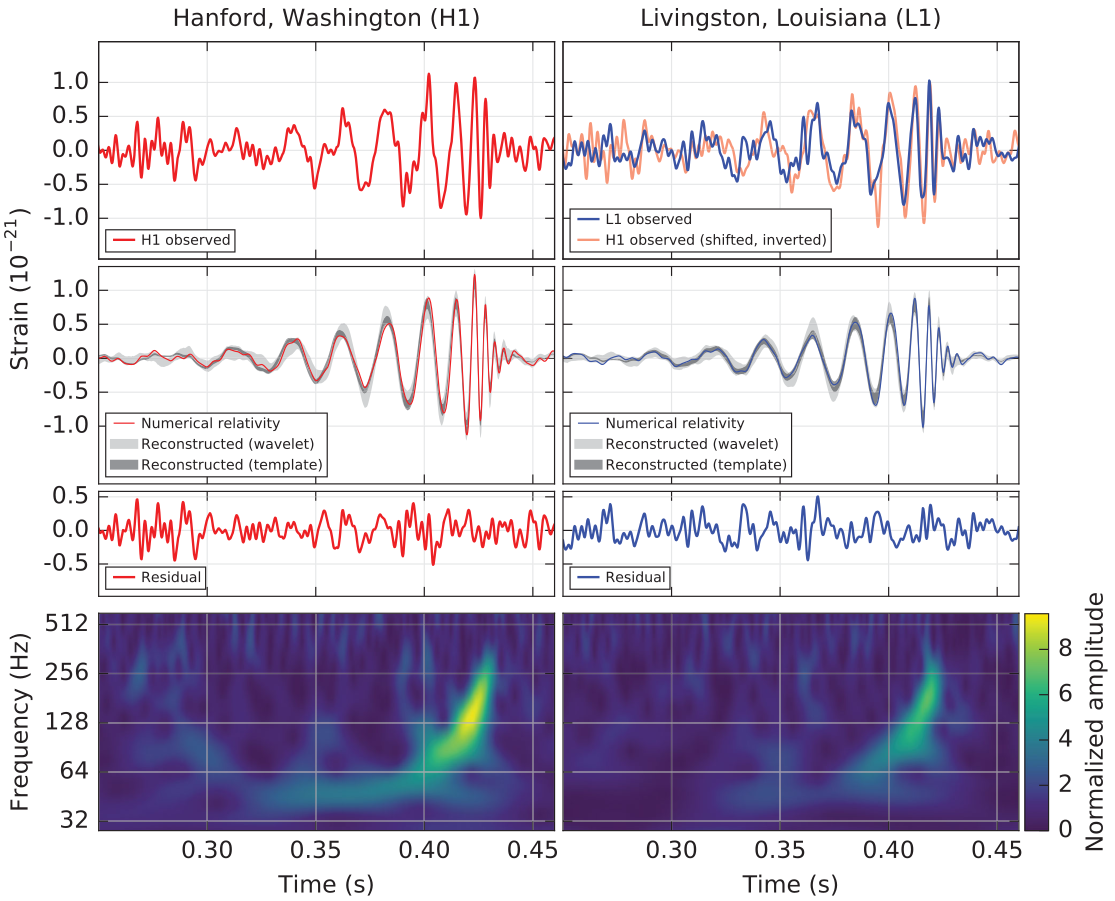
\includegraphics[width=\textwidth]{./images/GW150914.png}
	\caption{Signal detection of GW150914 \cite{Abbott2016firstGW}. \textit{Top:} amplitude time-series. \textit{Bottom:} frequency time-series.}\label{fig:GW150914}
\end{figure}

\paragraph{GW150914-like binaries} It is possible to apply the above formulas to get an order-of-magnitude estimate of any binary detection. For instance, the Bayesian analysis of the signal of GW150914 reported in Fig.\ \ref{fig:GW150914} revealed two black holes of masses $M_1=35.6^{+4.7}_{-3.1} ~ \msun$ and $M_2=30.6^{+3.0}_{-4.4} ~ \msun$ at redshift $z=0.09^{+0.03}_{0.03}$ within 90\% confidence intervals \cite{GWTC-1}. Using Eq.\ \ref{eq:Massesredshift}, the masses revealed in the detector frame where about 10\% heavier, respectively $M_1 \sim 39 ~ \msun$ and $M_1 \sim 33 ~ \msun$. The corresponding chirp mass was $\mathcal{M} \sim 30 \msun$ and the total mass $M \sim 70 ~ \msun$, meaning that at the coalescence the binary had a radius of only $R_{\rm coalescence} \sim 200~\text{km}$ and produced a peak gravitational wave at $\nu_{\rm GW, peak} \sim 300 ~\text{Hz}$. The binary had a luminosity distance of $d_L=410~\text{Mpc}$ and the gravitational wave was detected with an amplitude of $h \sim 10^{-21}~ \text{Hz}^{-1/2}$.


\begin{figure}[h]
	\begin{minipage}{.47\textwidth}
		\centering
		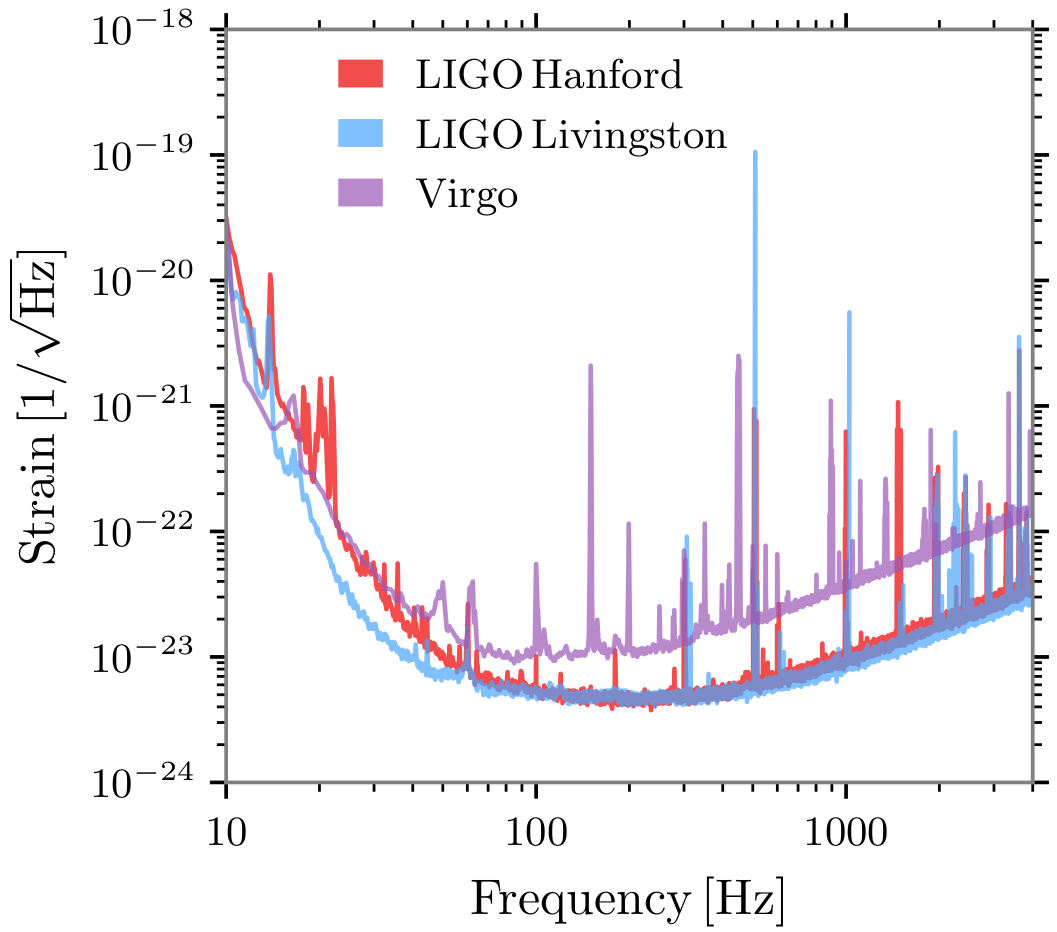
\includegraphics[width=\textwidth]{./images/sensitivity.png}
	\end{minipage}
	\hfill
	\begin{minipage}{.53\textwidth}
		\centering
		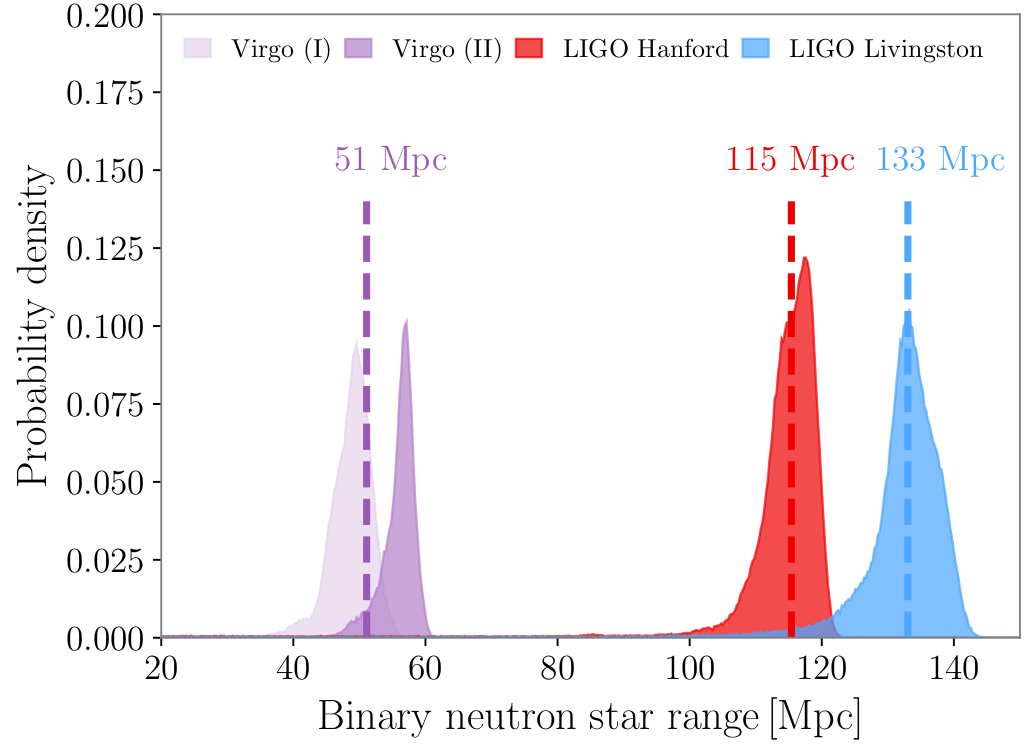
\includegraphics[width=1.02\textwidth]{./images/O3BNSrange.png}	
	\end{minipage}
	\caption{Sensitivity curves (\emph{left}) and binary neutron star observational probability density (\emph{right}) of the LIGO and Virgo interferometers during the third observing run O3. The lower sensitivity of Virgo for $\nu \gtrsim 150~\text{Hz}$ limits the observable volume, especially for the lighter sources like the binaries of neutron stars \cite{GWTC-3}.}\label{fig:O3sensitivity}
\end{figure}



\begin{figure}[h]
	\begin{minipage}{.49\textwidth}
		\centering
		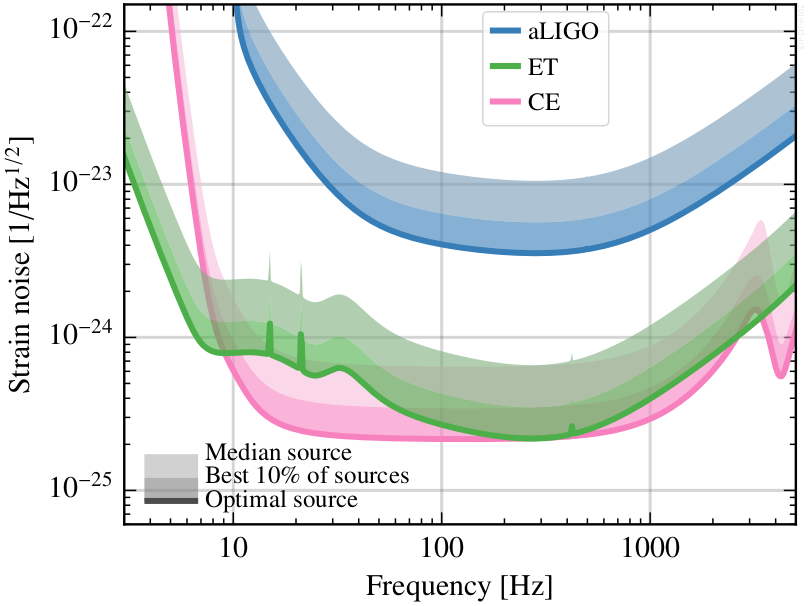
\includegraphics[width=\textwidth]{./images/ETsensitivity.png}
	\end{minipage}
	\hfill
	\begin{minipage}{.49\textwidth}
		\vspace{-2mm}
		\centering
		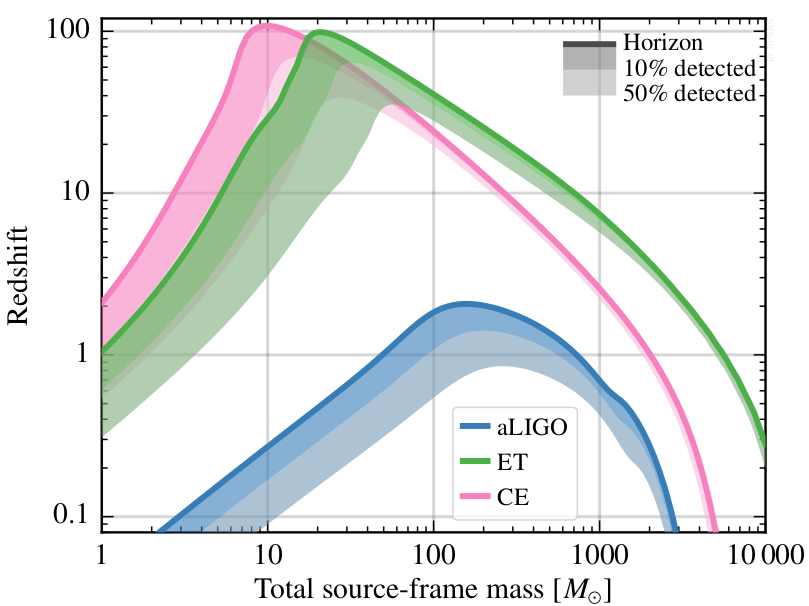
\includegraphics[width=1.02\textwidth]{./images/EThorizon.png}	
	\end{minipage}
	\caption{Example of the possible sensitivity curves (\emph{left}) and instrumental horizons (\emph{right}) of the planned third generation interferometers Einstein Telescope and Cosmic Explorer. Unlike the advanced LIGO interferometer, Einstein Telescope and Cosmic Explorer will detect \erika{binary black holes} well-beyond redshift $z \sim 2$ \cite{EThorizonsensitivity}.}\label{fig:ETsensitivity}
\end{figure}


\paragraph{Sensitivity, biases and future perspectives}
According to Eq.\ \ref{eq:h}, the farther the sources are, the lower the amplitude of the gravitational wave that reaches the detector.  To have a quantitative comparison it is useful to use as proxy-source a binary neutron star: the limits on its equation of state impose that a single neutron star has at maximum a mass of $\sim 3~\msun$, therefore the binary chirp mass is well-defined and doesn't exceed $\mathcal{M} \sim 2.6 ~\msun$ \cite{NSreview}. Fig. \ref{fig:O3sensitivity} reports the sensitivity curves of the LIGO and Virgo interferometers and the end of the third observing run O3, highlighting how the worst sensitivity of Virgo at the high frequency (mainly caused by the photon shot noise) limits the maximum observable distance of the binary neutron star by a factor of 2 when compared to the performances of LIGO \cite{GWTC-3}.

In terms of binary black holes, a source like GW150914 that peaks at $\nu \sim 300~\text{Hz}$ could be observed by the LIGO interferometers with sensitivity of $h \sim 10^{-23}~ \text{Hz}^{-1/2}$ up to a luminosity distance of $d_L \sim 1.6~\text{Gpc}$: the binary can now be observed in a volume of space $\sim 64$ times bigger. The observable volume is maximum for binaries that merge close to the best sensitivity range at $\sim 100-200~\text{Hz}$, that, according to Eq.\ \ref{eq:nupeak} are likely binaries composed of heavy black holes with a total mass  $M_1+M_2 \sim 60-100~\msun$: the gravitational wave detectors are biased towards the observation of heavy binary black holes.


Third generation gravitational wave detectors, like the planned Einstein Telescope and Cosmic Explorer, will be at least one order of magnitude more sensible than advanced LIGO and Virgo at design sensitivity, allowing to probe binary compact object mergers beyond redshift $z \sim 2$. As shown in Fig.\ \ref{fig:ETsensitivity}, the maximum observable distance depends on source mass and interferometers' sensitivity, that ultimately depends on its design (Fig.\ \ref{fig:ETsensitivity} is only one of the proposed designs, but is representative of the goals of the project)  \cite{EThorizonsensitivity}. Again, Eq.\ \ref{eq:h} underlines how the detection improvement is mainly for \erika{binary black holes}: their heavier mass produces stronger amplitude signals than binary neutron stars, making them visible even at high redshift.



\subsection{Observed distributions of mass and spin}\label{subsec:GWmassspin}

\paragraph{Merger rate densities and posterior distributions}% pluto, ho riscritto il paragrafo
\erika{The parameter distributions of the observed gravitational wave sources are usually expressed either in terms of cumulative density functions (CDFs) or in terms of \emph{merger rate densities} (MRDs), the latter being the number of sources that merge in a co-moving volume and in a given time range. Both distributions are derived as posterior distribution functions (PDFs) $p(\theta)$ of some parameter $\theta$ in the framework of an hierarchical Bayesian analysis, that accounts for the observational biases and fits the hyper-parameters $\Lambda$ for the intrinsic population properties. From a theoretical perspective, the hyper-parameter fits are one of the most fundamental information to extract from the observations: their values can be directly compared with the predictions of the population-synthesis codes, discriminating between the different models proposed for the formation of the compact object merges \cite{GWTC-3_interpretation, BayesforGW}.} \\

\erika{The astrophysical PDF of the source parameter $\theta$ is calculated averaging the prior distribution of the source $\pi(\theta|\Lambda)$ over the population hyper-parameters $\Lambda$ }

\begin{equation}\label{eq:posteriorMRD}
    p(\theta) = \int \pi(\theta|\Lambda)~p(\Lambda|\vec{d})~\rm d \Lambda
\end{equation}

\erika{The prior $\pi(\theta|\Lambda)$ is the intrinsic distribution of the source parameter $\theta$ for a given set of hyper-parameters $\Lambda$. The hyper-posterior $p(\Lambda|\vec{d})$ indicates the most probable values for the hyper-parameters $\Lambda$ given the observed data vector $\vec{d}$. Intuitively, the hyper-posterior could be a Gaussian that shifts and tightens around the true values of the hyper-parameters the more data are collected i.\ e.\ the more the data are representative of the population of interest.}

\erika{To be more clear, it is possible to consider as an example a posterior distribution of the primary mass $p(M_1)$ similar to the one shown in the left-hand panel of Fig.\ \ref{fig:primarymassspectrum}. A reasonable choice for the prior could be a power-law (possibly related to the power-law of the initial mass functions of the stars \cite{Kroupa2001}) plus a Gaussian $\mathcal{N} (\mu,\sigma)$ centered in $\mu$ with dispersion $\sigma$ (to indicate possible over-densities)} % lo so che ci sarebbe anche una massa minima per il modello vero, ma qui sto solo facendo un "esempio didattico" semplice

\begin{equation}\label{eq:priormassprimary}
    \pi(M_1|\alpha,\mu,\sigma) \propto M_1^{-\alpha}~\mathcal{N} (\mu,\sigma)
\end{equation}

\erika{The three hyper-parameters $\vec{\Lambda} = (\alpha,\mu,\sigma)$ will be then determined by the fit to the data. Since population-synthesis codes too can predict the intrinsic distribution of the primary masses $p(M_1)$, it is possible to reject the results and the corresponding underlying assumptions of the ones that, for instance, predict a Gaussian peak in a different position than the one obtained from the hyper-parameter fits.}\\


\erika{According to Bayes theorem, the hyper-posterior $p(\Lambda|\vec{d})$ is proportional to the hyper-likelihood $\mathcal{L}(\vec{d}|\Lambda)$ an to the hyper-prior $\pi(\Lambda)$}

\begin{equation}\label{eq:hyperposterior}
     p(\Lambda|\vec{d}) \propto~\mathcal{L}(\vec{d}|\Lambda)~\pi(\Lambda)
\end{equation}

\erika{The hyper-prior $\pi(\Lambda)$ indicates the prior beliefs on the hyper-parameters $\Lambda$ and usually is assumed to be uniform and non-informative. The hyper-likelihood $\mathcal{L}(\vec{d}|\Lambda)$ is the key quantity determined by the data and accounts for the observational biases. Assuming that the number of detected gravitational-waves $N_{\rm det}$ is related to the intrinsic number of events through a Poisson statistics, the hyper-likelihood can be modelled as}

\begin{equation}\label{eq:hyperlikelihood}
    \mathcal{L}(\vec{d}, N_{\rm det}| \Lambda) \propto N^{N_{\rm det}}~e^{-N\xi(\Lambda)} ~\prod_{i=1}^{N_{\rm det}} \int \mathcal{L}(d_i|\theta)~\pi(\theta|\Lambda)~\rm d\theta
\end{equation}

\erika{The product $N^{N_{\rm det}}~e^{-N\xi(\Lambda)}$ encodes the information on the observational biases and detection efficiency. In fact, $N$ indicates the expected number of mergers over the observation period while $\xi(\Lambda)$ is the fraction of mergers that are detectable for the population characterized by hyper-parameters $\Lambda$. $N^{N_{\rm det}}~e^{-N\xi(\Lambda)}$ is strongly influenced by the dimension of the co-moving time-volume $\langle V\,T\rangle$ explored by the detector, namely the instrumental horizon integrated for the observation time.}

\erika{The single-event likelihood $\mathcal{L}(d_i|\theta)$ is usually obtained via importance sampling from a default prior $\pi_{\rm def}(\pi)$. Therefore, the integral of the prior $\pi(\theta|\Lambda)$ over the single-event likelihood $\mathcal{L}(d_i|\theta)$ can be evaluated averaging over the posterior samples}

\begin{equation}
   \int \mathcal{L}(d_i|\theta)~\pi(\theta|\Lambda)~\rm d\theta \approx \langle~ \frac{\pi(\theta|\Lambda)}{\pi_{\rm def}(\pi)}~\rangle
\end{equation}


\begin{figure}
	\begin{minipage}{.60\textwidth}
		\centering
		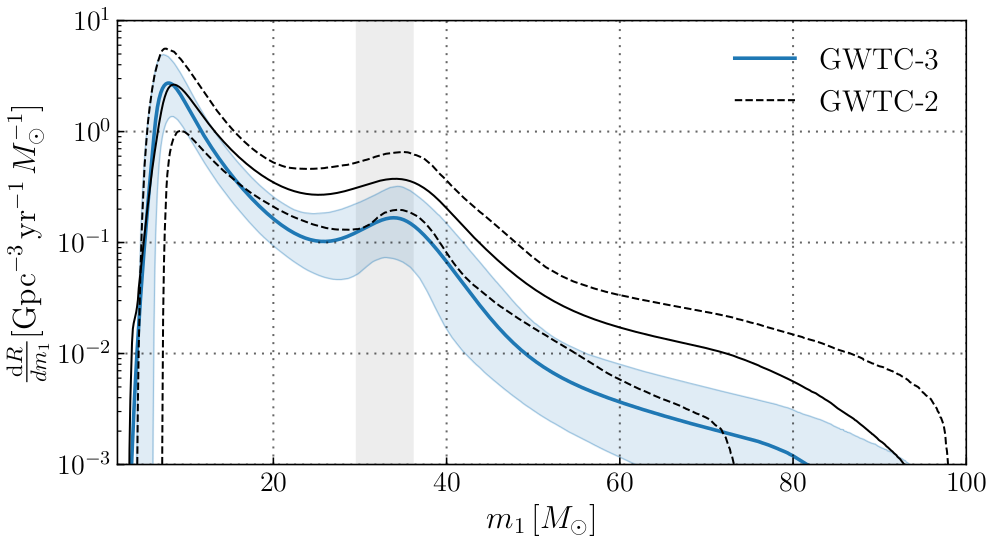
\includegraphics[width=\textwidth]{./images/MassMergerRate.png}
	\end{minipage}
	\hfill
	\begin{minipage}{.39\textwidth}
		\vspace{1mm}
		\centering
		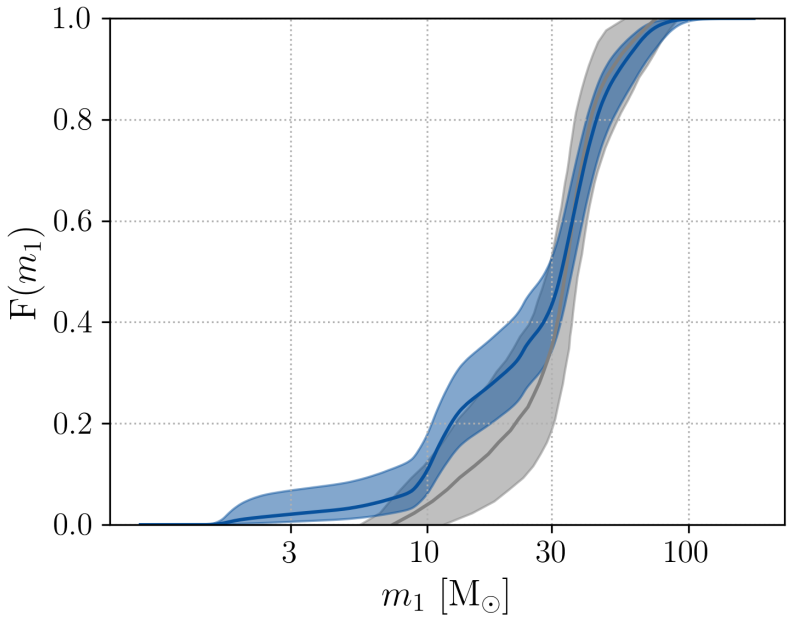
\includegraphics[width=\textwidth]{./images/MassCumulative.png}	
	\end{minipage}
	\caption{Differential merger rate density  (\emph{left}) and cumulative density function (\emph{right}) of the primary mass of the \erika{binary black holes} detected with the gravitational waves. In blue the posterior distributions obtained with GWTC-3, in grey the ones obtained with GWTC-2. The thick solid lines denote the median values and are surrounded by the 90 \% credible intervals.The vertical grey band on the differential merger rate indicates the 90 \% credible interval for the mean of the Gaussian peak \cite{GWTC-3_interpretation}.}\label{fig:primarymassspectrum}
\end{figure}


\paragraph{Primary mass spectrum}
For each binary source, the primary mass is defined as the most massive compact object. The differential merger rate density of the primary mass observed at the end of O3b is a power-law with slope $\alpha = 3.5_{-0.56}^{+0.6}$ with a Gaussian peak centered in $M_{\rm 1,\mu} = 34_{-4.0}^{+2.6}~ \msun$. GWTC-3 contains more low-mass system than GWTC-2, causing a steeper decline in the power law at higher masses and reducing the mass of the 99th percentile, now at $\sim 44~\msun$ and not at $\sim 60~\msun$ as it was in GWTC-2. There are strong over-densities at $\sim 10~\msun$ and $\sim 35~\msun$ that may reflect properties of the astrophysical environment but that are still under investigation.

Even though the region $\gtrsim 70~\msun$ is still weakly explored, there is no strong evidence for or against an upper mass gap, at least up to $\sim 75~\msun$. Still, a similar finding challenges the existence of the pair-instability mass gap ($\sim 60 - 120~\msun$ \cite{spera2017_pisnSNe}): either the single stellar evolution models need to be corrected \cite{MassGapStellarEvo_Costa2021} or the formation in dynamically active environments is required \cite{Rastello2021_dynamics}. On the other hand, there is still mild support for a lower-mass gap between $\sim 3~\msun$ and $\sim 5~\msun$, potentially due to the physics of core-collapse supernovae and in agreement with the dearth of compact objects observed in nearby X-ray binaries \cite{massgapreal_ozel2010}.




\paragraph{Spin distribution}
At the end of the third observing run, the black hole population exhibits a preference for low-spinning black holes $\chi \lesssim 0.4$, with a peak distribution at $\chi \sim 0.2$ and a long tail at higher values. Separate analysis of the fastest ($\chi_A$) and slowest ($\chi_B$) spinning components of the binary revealed that the rapid-spinning components are still quite slow $\chi_A \sim 0.4$ while the slow-spinning ones are concentrated below $\chi_B \sim 0.2$, as expected. Posterior distributions for the spin magnitudes are shown in Fig.\ \ref{fig:spinmagnitude}.

% ho un po' riaggiustato visto che dicevi che non ti era del tutto chiaro
\erika{As shown in the left-hand panel of Fig.\ \ref{fig:spineffective}, the effective spin parameter $\chi_{eff}$ distribution is still consistent with a Gaussian centered in $\chi_{eff, \mu} = 0.06_{-0.05}^{+0.04}$ with a peak still compatible with $\chi_{eff} = 0$, indicating either very low spin magnitudes or spins misaligned with the orbital angular momentum. In particular, the distribution extends to negative effective spins $\chi_{eff} < 0$, suggesting the existence of polar angle tilts $\theta \geq 90^\circ $ i.\ e.\ black holes anti-aligned with the orbital angular momentum that likely formed in dynamically active environments. This evolutionary scenario is consistent also with the flatter and more isotropic-oriented distribution of the tilt angles shown in the right-hand panel of Fig.\ \ref{fig:spineffective}. }



\begin{figure}[h!]
	\begin{minipage}{.49\textwidth}
		\centering
		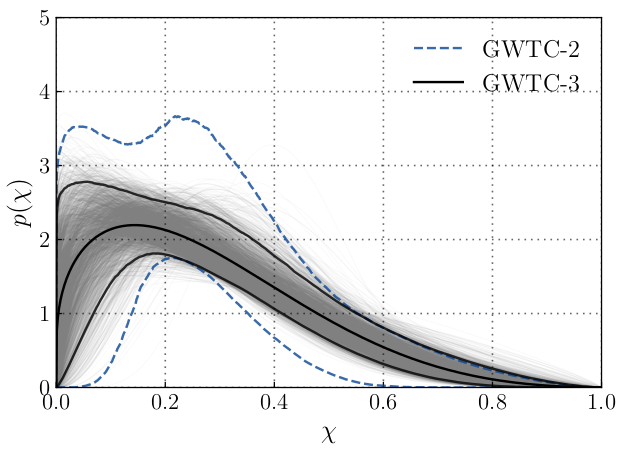
\includegraphics[width=\textwidth]{./images/spinmagnitude.png}
	\end{minipage}
	\hfill
	\begin{minipage}{.49\textwidth}
		\vspace{0.8mm}
		\centering
		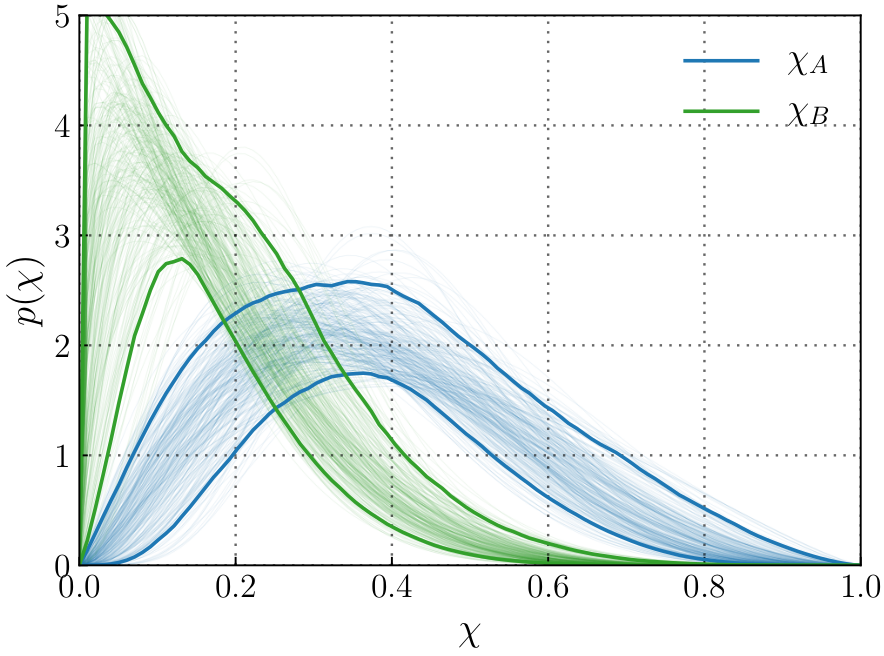
\includegraphics[width=0.975\textwidth]{./images/spinmagnitudehighlow.png}	
	\end{minipage}
	\caption{\emph{Left:} Spin magnitude ($\chi$) posterior distribution of all the merging black holes in GWTC-3 (gray) compared to the 90 \% credible intervals for GWTC-2 (in blue). \emph{Right:} Separate posterior distributions within 90 \% credible bounds of the fastest ($\chi_A$, in blue) and slowest ($\chi_B$, in green) black holes in the binary. The new observations indicate a preference for slow-spinning black holes $\chi \lesssim 0.4$, with a fast-spinning component still rather slow $\chi_A \sim 0.4$ \cite{GWTC-3_interpretation}} \label{fig:spinmagnitude}
\end{figure}


\begin{figure}[h!]
	\begin{minipage}{.49\textwidth}
		\centering
		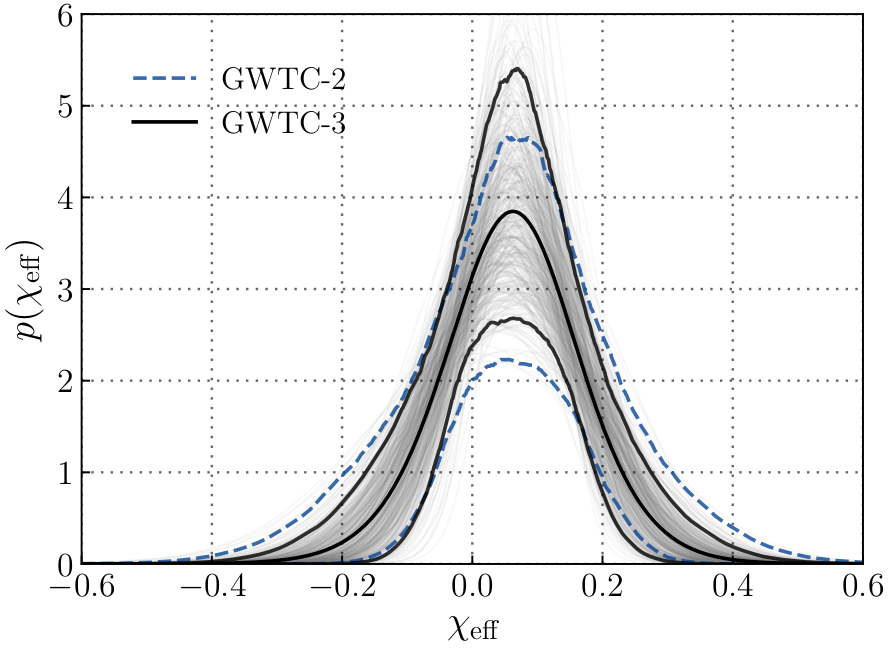
\includegraphics[width=\textwidth]{./images/spineff.png}
	\end{minipage}
	\hfill
	\begin{minipage}{.49\textwidth}
		\vspace{-1mm}
		\centering
		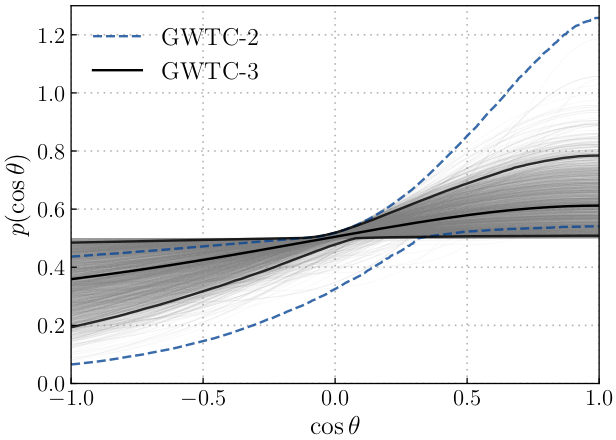
\includegraphics[width=0.96\textwidth]{./images/spinorientation.png}	
	\end{minipage}
	\caption{\emph{Left:} Gaussian posteriors of the effective spin $\chi_{eff}$ of all the merging black holes in GWTC-3 (gray) compared to the 90 \% credible intervals for GWTC-2 (blue). \emph{Right:} Posterior distribution of the polar angle $\theta$ of all the merging black holes in GWTC-3 (gray) compared to the 90 \% credible intervals in GWTC-2 (blue) \cite{GWTC-3_interpretation}.} \label{fig:spineffective}
\end{figure}

\begin{figure}[h!]
	\begin{minipage}{.49\textwidth}
		\centering
		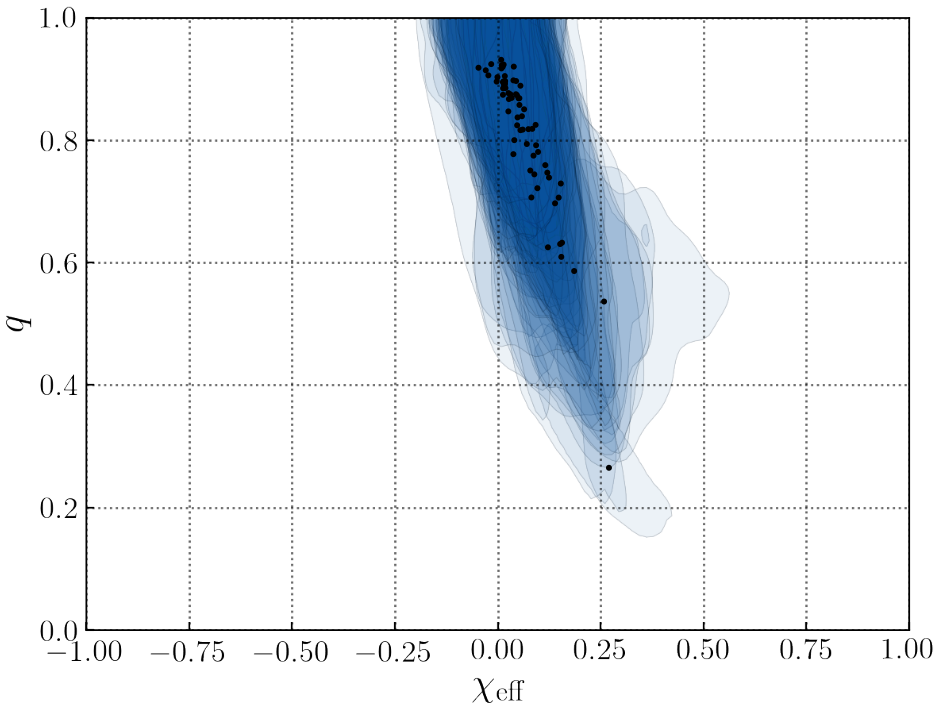
\includegraphics[width=\textwidth]{./images/spinmassratio.png}
	\end{minipage}
	\hfill
	\begin{minipage}{.49\textwidth}
		%\vspace{-2mm}
		\centering
		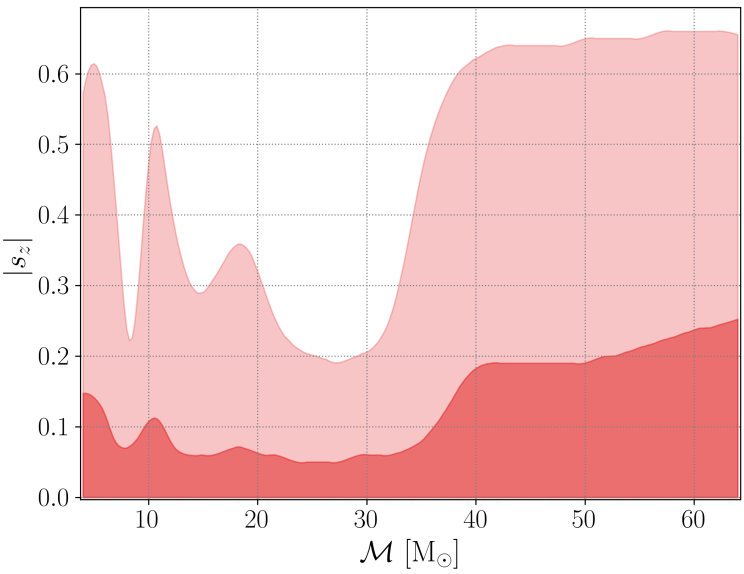
\includegraphics[width=0.95\textwidth]{./images/spinchirpmass.png}	
	\end{minipage}
	\caption{\emph{Left:} Effective spin $\chi_{eff}$ anti-correlating with the mass ratio $q$. Black points mark the median of the PDF obtained using an informed prior where mean and standard deviation of the Gaussian posterior of $\chi_{eff}$ were allowed to evolve with $q$. Blue shaded areas indicate the 90 \% credible intervals for each median point. \emph{Right:} Spin component parallel or anti-parallel to the orbital angular momentum vector $\vec{s}_z$ as a function of the binary chirp mass. Light (dark) shaded areas indicate 90 \% (50 \%) credible intervals \cite{GWTC-3_interpretation}.}\label{fig:spincorrelations}
\end{figure}



Data from GWTC-3 exhibit a mild anti-correlation between the effective spin parameter $\chi_{eff}$ and the mass ratio $q$, as shown in the left-hand panel of Fig.\ \ref{fig:spincorrelations}. If confirmed, the anti-correlation would challenge the usual evolutionary pathways for binary black hole progenitors, indicating that field binaries formed with $q \sim 1$ do not have spins aligned with the orbital angular momentum ($\chi_{eff} \sim 1$),  because either the tides and mass transfer are not so efficient or there is some additional and yet unknown effect, like a third-body perturbation \cite{misalignedbinary}.


So far the LVC analysis has been carried out assuming the same spin distribution at all masses, even though the low-mass binaries dominate the sample and seven high-mass binaries make up $\sim 70 \%$ of the moderate spins. A more refined analysis compared the spin component aligned with the orbital angular momentum $|s_z|$ with the chirp mass of each binary. The result is shown in the right-hand panel of Fig.\ \ref{fig:spincorrelations}. All the binaries are consistent with spins misaligned with the orbital angular momentum ($|s_z| = 0$) even tough there are over-densities in the chirp mass distribution: \st{if confirmed by further detections it would challenge the correlations predicted by the hierarchical formation scenario} \micmap{no un attimo, questa frase dove l'hai trovata? è vero che i bbh gerarchici tendono ad avere spin $\sim{0.7}$ più o meno isotropicamente distribuito - il meno è per gli AGN disk - ma nessuno si immagina una correlazione, semmai una sottopopolazione di gerarchici. Finora abbiamo solo GW190521 che sia affidabile} \erika{Fine della sezione A pag 36 del paper sull'interpretazione di GWTC-3  (https://ui.adsabs.harvard.edu/abs/2021arXiv211103634T/abstract) Cito la frase che ammetto aver quasi copiato ciecamente " Figure 19 (la mia 1.7 dx) suggests aligned spin magnitude remains constrained to be close to zero independently of the most well-identified peaks in the mass distribution, contrary to what would be expected from hierarchical formation scenarios for these peaks [110, 197–201]."}. The large spread of the high-mass binaries $\mathcal{M} \gtrsim 30~\msun$ with respect to the low-mass ones is consistent with having a large number of detections at low masses and fewer at high masses: at the moment it is not possible to reject or confirm an aligned spin magnitude dependence with the chirp mass.











\section{X-ray binaries}

\subsection{X-ray binaries hosting a black hole}\label{subsec:XraybinariesSED}

\paragraph{The best way to observe a black hole}
X-ray binaries that host a black hole and a massive star are currently the best observational candidates as binary black hole progenitors: not only such systems are already in a binary configuration but the accretion onto the compact object powers an X-ray emission that allows us to observe them \cite{Xbinaries_massmeasure}. The possibility to observe them is precisely the key property of X-ray binaries: even though $\sim 70 \%$ of massive stars are born in binary systems \cite{Sana2012}, most black holes are quiescent and can be observed only with accurate measurements of their radial velocity or proper motions \cite{BHnoninteracting_Giesers2018}. Isolated black holes, that could dynamically exchange with a binary, are even more difficult to observe and currently the best detection technique for them is microlensing \cite{BHmicrolensing}.

\paragraph{LMXBs and HMXBs}
The mass of the non-degenerate donor star and the type of accretion determine two sub-classes of X-ray binaries hosting a black hole: low-Mass X-ray binaries (LMXBs) and high-mass X-ray binaries (HMXBs). LMXBs typically host low-mass stars $\lesssim 2-3~\msun$ that fill their Roche lobe. In contrast, HMXB  donors are more massive stars $\gtrsim 5~\msun$ that typically do not fill their Roche lobe but become wind-fed systems. Up-to-date, about $\sim 30$ X-ray binaries are estimated to host a black hole \cite{HMXBH_spins2021}.

\paragraph{Spectral energy distribution in the X-rays}
The X-ray spectral energy distribution of an X-ray binary is dominated by the emission of the accretion disk surrounding the compact object. A classic Shakura-Sunyaev accretion disk around a stellar-sized compact object emits most of its photons in the UV/soft X-ray regime $\sim 10^{2}-10^{4}$ keV with an X-ray luminosity $L_X \gtrsim 10^{37}~\text{erg s}^{-1}$, has an effective radiation temperature of $\sim 10^{7}-10^{8}~K$ and produces a thermal multi-color black-body continuum \cite{S&S1973_accretiondisk}. Usually, accretion disks are surrounded by a corona of hot thermal electrons: photons in the low energy tail of the disk thermal emission (soft optical/UV) that encounter the corona suffer multiple inverse Compton scatterings (i.\ e.\ suffer a thermal Comptonization) and are re-emitted in the form of a hard X-ray power-law spectrum. Part of the X-ray power-law radiation is directly emitted towards the observer at infinity but another part is re-emitted back to the accretion disk, reprocessed by it and eventually reflected at the infinity. 
 
The X-ray photons reprocessed by the corona are more energetic than the ones originally produced in the accretion disk and see the disk as a slab of cold gas, interacting with it mainly through Compton scattering and photoelectric absorption followed by fluorescent line emissions. On the one hand, the energy dependence of the photoelectric absorption favours the absorption of the soft X-rays, causing a down-scaling in the corresponding region of the reflected continuum. One other hand, the hard X-rays are Compton-scattered back, thus reflected towards the observer at the infinity, except for the ones more energetic than $\sim 20-30$ keV, which suffer Compton recoil. Overall, the X-ray continuum due to reflection is characterized by a hump at $\sim 20$ keV and by the fluorescent lines emitted by the ionized heavy elements, mainly iron. The 6.4 keV line of the Fe K$\alpha$ line is the strongest fluorescent line and is caused by the absorption of an incident photon with energy larger than 7.1 keV, as shown in the right-hand panel of Fig. \ref{fig:accretiondisk}.

The X-ray continuum seen by an observer at infinity can be divided into soft and hard X-ray regimes, respectively below or above 10 keV. The soft X-ray spectrum is dominated by the thermal continuum of the disk and exhibits a multi-color black body shape peaked at $\sim 2$ keV. The hard X-ray spectrum is determined by the radiation reprocessed by the hot corona: the hard power-law of the photons directly emitted from the corona is modulated by the hump at $\sim 20$ keV and the fluorescence emission lines caused by the additional reflection on the accretion disk, as shown in the left-hand panel of Fig. \ref{fig:accretiondisk} \cite{FeKalphaline_Fabian2000}.


\begin{figure}
	\begin{minipage}{.58\textwidth}
		\centering
		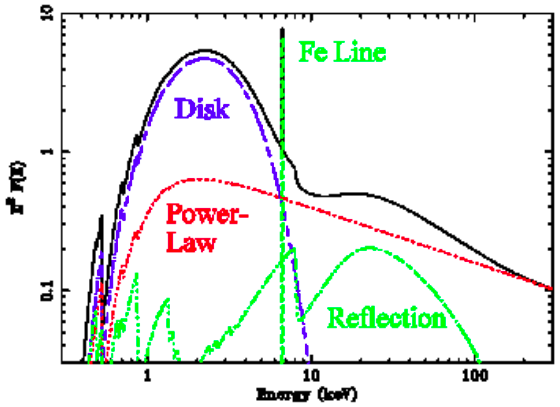
\includegraphics[width=\textwidth]{./images/accretiondiskSED.png}
	\end{minipage}
	\hfill
	\begin{minipage}{.42\textwidth}
		%\vspace{-2mm}
		\centering
		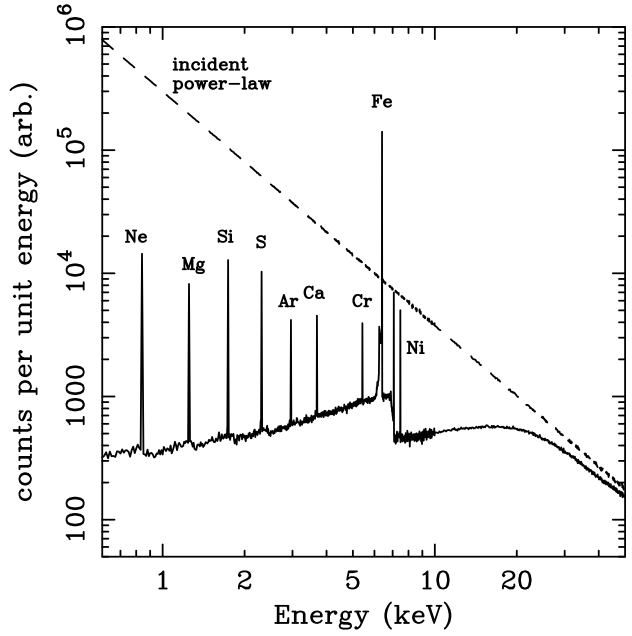
\includegraphics[width=\textwidth]{./images/accretiondiskFeKalphaline.png}	
	\end{minipage}
	\caption{\emph{Left:} Sketch of the dominant components in the spectral energy distribution of an X-ray binary. In the soft X-rays, the emission is dominated by the thermal continuum of the disk, visible as a multi-color black-body peaked at $\sim 2$ keV. In the hard X-rays, the radiation reprocessed by the corona is either directly emitted towards the observer as a power-law or is reflected by the disk, causing a hump at $\sim 20$ keV and the strong fluorescent Fe K$\alpha$ line at $6.4$ keV. Credit: J. Miller \emph{Right:} Montecarlo simulation of the X-ray spectrum reflected by a cold slab of gas. An incident power-law radiation (dashed line) is damped in the soft X-rays, exhibiting strong fluorescent lines and a hump before the cut-off due to Compton recoil \cite{FeKalphaline_Fabian2000}.}\label{fig:accretiondisk}
\end{figure}

\subsection{Measuring the properties of  X-ray binaries}\label{subsec:Xraymeasure}
\paragraph{Masses, period and inclination}
Inspection of the radial velocity and X-ray light curves provides essential information to characterize the orbital properties of X-ray binaries. The orbital period can directly be obtained from the periodicity of the light and velocity curves and often is the most-accurate orbital parameter. The mass estimate of the compact object is less precise and relies on the determination of other uncertain quantities, \erika{like the companion mass, binary mass ratio, inclination and distance.}

The dynamical method is the most robust and common procedure to determine the mass of an object in a binary system. Its application is limited to the systems that satisfy three conditions: the companion star is visible in the optical/near-infrared band, single spectral lines can be identified in its optical/near-infrared spectrum (resolving power $\lambda/\Delta \lambda \gtrsim 1500$), at least one photospheric absorption line can be used as a proxy for the orbital motion. Therefore, the dynamical method cannot be applied to distant X-ray binaries (not enough resolving power), to systems with a companion not visible in the optical/near-infrared band and, most importantly, to systems subject to outbursts or strong stellar winds. These limitations prevent the application of the dynamical mass determination to many HMXBs. For instance, as explained in Sec.\ \ref{sec:WRBHobserved}, the strong winds of the  Wolf-Rayet star coupled with the X-ray variability of the compact object caused the revision of several important dynamical mass measurements in the Wolf -Rayet -- black hole binaries \cite{ICX10X-1_Laycock2015_revisited}.

Alternative techniques for the mass measurement are available but still require a good calibration, as for the case of the scaling relations with the X-ray spectral and timing properties in presence of quasi-periodic oscillations \cite{Xbinaries_massfromXtiming}.\\

According to the dynamical method, the spectral lines that trace the orbital motion are used to build the velocity curves and extract the orbital period $P_{orb}$ and the radial velocity semi-amplitude $K_c$ of the companion star. Kepler's third law corrects the measures for the inclination angle $i$ and the mass ratio $q=M_c/M_{\rm BH}$ and couples them into the \emph{mass function} $f(M)$: a non-linear expression relating the masses of the companion star $M_c$ and of the compact object $M_{\rm BH}$:

\begin{equation}\label{eq:massfunction}
	f(M) = \frac{K_c^3 P_{\rm orb}}{2 \pi G} = \frac{M_{\rm BH}^3 \sin^3 i}{(M_{\rm BH} + M_c)^2} = \frac{M_{\rm BH}^3 \sin^3 i}{(1+q)^2}
\end{equation}

The above formula is for a circular binary: a reasonable assumption for a system that likely already had time to circularize, given that its X-ray emission is the result of a mass-transfer process. Eventually, the mass of the black hole in the binary can be determined with further assumptions and measurements on the mass ratio $q$ (or, alternatively, on the companion mass $M_c$) and on the inclination of the system $i$.\\

The mass ratio can be determined assuming a spherically symmetric star that fills its Roche lobe in a tidally locked system. Under these conditions, the rotational broadening ($V \sin i$) of the absorption lines in the stellar photosphere can be related to the mass ratio $q$ of the system \cite{Xbinaries_qmeasure}

\begin{equation}\label{eq:qmeasure}
	\frac{V \sin i}{K_c} \sim 0.462~q^{1/3} (1+q)^{2/3} 
\end{equation}

The measurement of $q$ is not always feasible and usually leads to under-estimate its value. The main uncertainty arises from the assumption of spherical symmetry in a Roche lobe filling system that, on the contrary, has tidal distortions. Moreover, the rotational broadening is usually of $\sim 30-120~\text{km s}^{-1}$ and requires a very large resolving power $\lambda/\Delta \lambda \gtrsim 5000$ to be measured, limiting the determination of $q$ only to the nearest binaries. 

For many systems, including the HMXBs that are not filling their Roche lobe, the mass function is not calculated with the mass ratio but with the companion mass. Fits on the stellar spectrum or mass-luminosity relations can provide the mass of the companion star. \erika{Usually the mass-luminosity relations are empirically obtained either by calibrations on synthetic spectra based on single stellar evolution models or by extrapolating the star properties from their position in the color-magnitude diagram (see Sec.\ \ref{subsec:massWR} for an example of a mass-luminosity relation for the Wolf-Rayet stars). The methodology requires a good modelling of stellar photospheres and optical/infrared emissions. However, strong winds and mass transfer events that expose the inner layers of the star or super-Eddington accretion onto the compact object may change the optical/infrared properties of the X-ray binary, leading to an uncertain estimate of the mass of the non-degenerate star \cite{superEddingtonaccBH_Ambrosi2018}. }

The inclination angle $i$ is usually obtained fitting the optical/near-infrared light curves with synthetic ellipsoidal models. Assuming that the companion star is filling its Roche lobe, tidal deformations of the star surface are expected to modulate the light curve profile and the amplitude of the modulation can be linked to the inclination angle. The light curve modulation can be affected by many sources of error (outburst, winds, etc.) and requires a very complex modeling, resulting in inaccurate determinations of the inclination angle. \erika{A similar, uncertain, result can be obtained also assuming that the inclination of the black hole high energy jet is the same of the binary: observations on the MAXI J1820+070 X-binary showed that spin-orbit misalignments can be $\gtrsim 40^{\circ}$ \cite{BHspinmisaligned_2022}.} Unless the system is an eclipsing binary, its inclination angle is poorly constrained and, given the cubic dependence in the mass function of Eq.\ \ref{eq:massfunction}, provides the biggest source of uncertainty in the black holes mass determination \cite{Xbinaries_massmeasure}.\\


HMXBs usually do not fill their Roche lobe and power the accretion through strong stellar winds: not only the method just described would provide very uncertain determinations for the inclination angle and companion mass but it would result in a very imprecise measure of the black hole mass. Therefore, the mass of the compact object in HMXBs is usually the result of a multi-parametric fit to the radial velocity curve and to the optical/near-infrared and X-ray light curves. The distance of the source is one of the parameters included in the multi-parametric model and the fit result is very sensible to it. For instance, recent radio astrometric distance measurements re-defined Cyg X-1 as a system hosting an O-type star of $\sim 40~\msun$ with a black hole of $\sim 21~\msun$, making it the most massive black hole detected so far in an X-ray binary \cite{cygnusx1}.




\paragraph{Spin}
Two techniques are generally used to measure the spin of black holes and require a fit to the X-ray spectrum of the accretion disk, either on the continuum or on the Fe K$\alpha$ lines (see Sec.\ \ref{subsec:XraybinariesSED} for a more detailed description of the X-ray spectral energy distribution). Both methods assume a geometrically thin and radiatively efficient disk, with emission that terminates at the innermost stable circular orbit (ISCO) \cite{Xbinaries_spinBHmeasure}.\\

The Fe K$\alpha$ line at 6.4 keV is a very strong fluorescent line produced by the X-ray radiation reflected from the accretion disk. In principle the line is very narrow but it is broadened by the Doppler effect, due to the disk rotation, and by the gravitational redshift, due to the vicinity to the black hole. Fast spinning Kerr black holes have an ISCO that is both closer to the black hole and more rapidly rotating, enhancing the gravitational redshift and the Doppler shift, respectively. As shown in the left-hand panel of Fig.\ \ref{fig:spinmeasure}, the spin of the black hole can be reconstructed by carefully fitting the broadening of the Fe K$\alpha$ line in the reflected X-ray spectrum.

The fit to the reflection spectrum has the great advantage of being a \textit{relative} measurement. Moreover, the spin determination can be carried out without knowing a priori the black hole mass, its distance and accretion rate, allowing the spins to be inferred in many systems with poorly constrained black hole masses \cite{HMXBH_spins2021}. On the contrary, the emissivity and ionization of the disk need to be already modeled to provide a good fit. Reflection spectra are also very sensitive to the inner disk inclination, although this information can be extracted by the same fit used for the Fe K$\alpha$ line.\\

Spin determination through the fit of the hard continuum relies again on having an ISCO of the disk closer to the black hole for high spin values. The thermal emission of the disk can be modeled as a multi-color black-body, where each anulus emits as a thermal black-body with radiation temperature $T \propto r^{-3/4}$ hotter for anuli closer to the black hole. Fast rotating black holes have accretion disks with ISCO very close to the black horizon that, being hotter, shift the peak of the multi-color emission towards higher energies: fitting the absolute shift in the flux emitted in the hard X-rays results in the spin determination, as shown in the right-hand panel of Fig.\ \ref{fig:spinmeasure}.

The method has many drawbacks, the main one being its necessity to fit the \textit{absolute} flux shift in a region where the emitted flux is strongly influenced also by the hard power-law emitted by the corona (see the left-hand panel of Fig.\ \ref{fig:accretiondisk} for a comparison): the choice of the hard component strongly impacts the spin value. Further sources of uncertainty come from the a priori knowledge of the inner disk inclination \erika{(in particular, the delicate assumption of spin and orbital angular momentum aligned \cite{BHspinmisaligned_2022})}, atmospheric scattering corrections and, most importantly, mass and distance of the black hole, required to have an accurate model for the absolute flux emitted by the disk \cite{Xbinaries_spinBHmeasure}.


\begin{figure}
	\begin{minipage}{.48\textwidth}
		\centering
		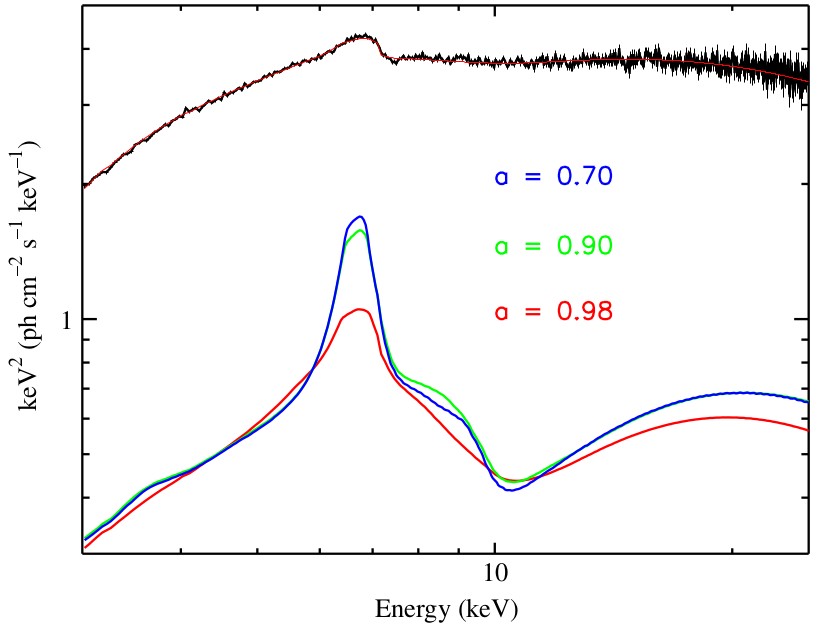
\includegraphics[width=\textwidth]{./images/spinreflection.png}
	\end{minipage}
	\hfill
	\begin{minipage}{.49\textwidth}
		%\vspace{-2mm}
		\centering
		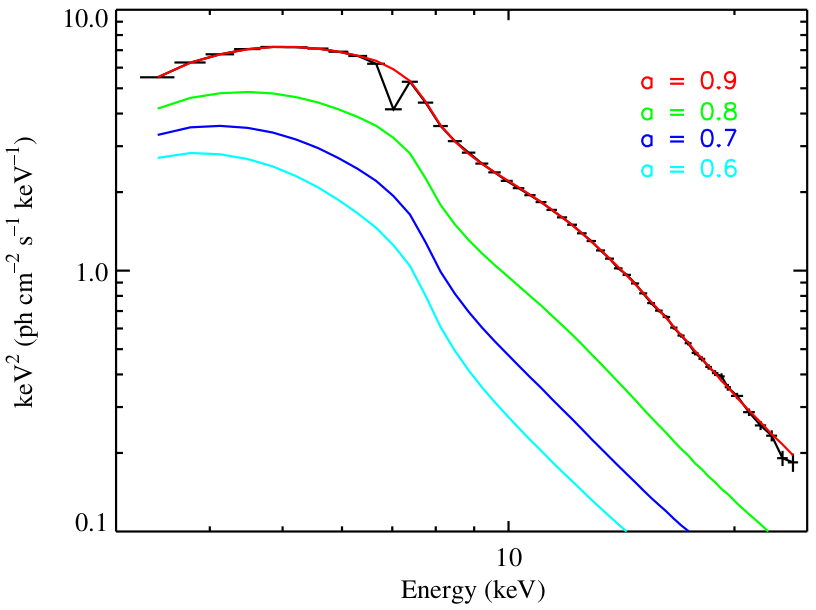
\includegraphics[width=\textwidth]{./images/spincontinuum.png}	
	\end{minipage}
	\caption{Example of the black hole spin measurement from fits to the Fe K$\alpha$ line (\emph{left}) or to the X-ray hard continuum (\emph{right}) of the candidate X-ray binary GRS 1915+ 105. The Fe K$\alpha$ fluorescent line causes the absorption at $\sim 7$ keV in the right-hand panel and results in a strong, broadened emission centered at 6.4 keV in the left-hand panel. The spectrum on the left is obtained with \textit{NuStar} while the one on the right with \textit{RXTE} \cite{GSR1915_lowhardXstate}.}\label{fig:spinmeasure}
\end{figure}


\section{Tensions in the underlying populations}%pluto
Up-to-date, one of the most detailed analysis of the mass and spin distribution of the underlying binary black hole populations compared the data of 44 binary black holes of the GWTC-2 catalogue with the only X-ray binaries with a reliable mass or \micmap{or o and? pensavo fosse and} \erika{or, di 29 spin noti di LMXBH solo 20 hanno anche la massa nota} spin measurement: 3 HMXBs and 29 LMXBs\erika{, of which only 20 have a reliable mass}  (see Sec.\ \ref{subsec:Xraymeasure} for a discussion on the main uncertainties in the X-ray parameter estimation) \cite{HMXBH_spins2021}. This study included as HMXBs the X-ray binaries with O-type donor star LMC X-1, M33 X-7 and Cyg X-1, excluding the Wolf-Rayet -- black hole binaries like NGC 300 X-1 or IC 10 X-1 because they have a less reliable mass measurements \cite{ICX10X-1_Laycock2015_revisited} (see the discussion in Sec.\ \ref{sec:WRBHobserved}). Even though the binary black hole sample is limited to GWTC-2 \cite{GWTC-2}, it is reasonable to expect that the same conclusions can be obtained using the GWTC-3 data, as discussed in Sec.\ \ref{subsec:GWmassspin}. In contrast, the limited sample of X-ray binaries with reliable mass and spin measurements causes the largest uncertainties.


\begin{figure}[h]
	\begin{minipage}{.49\textwidth}
		\centering
		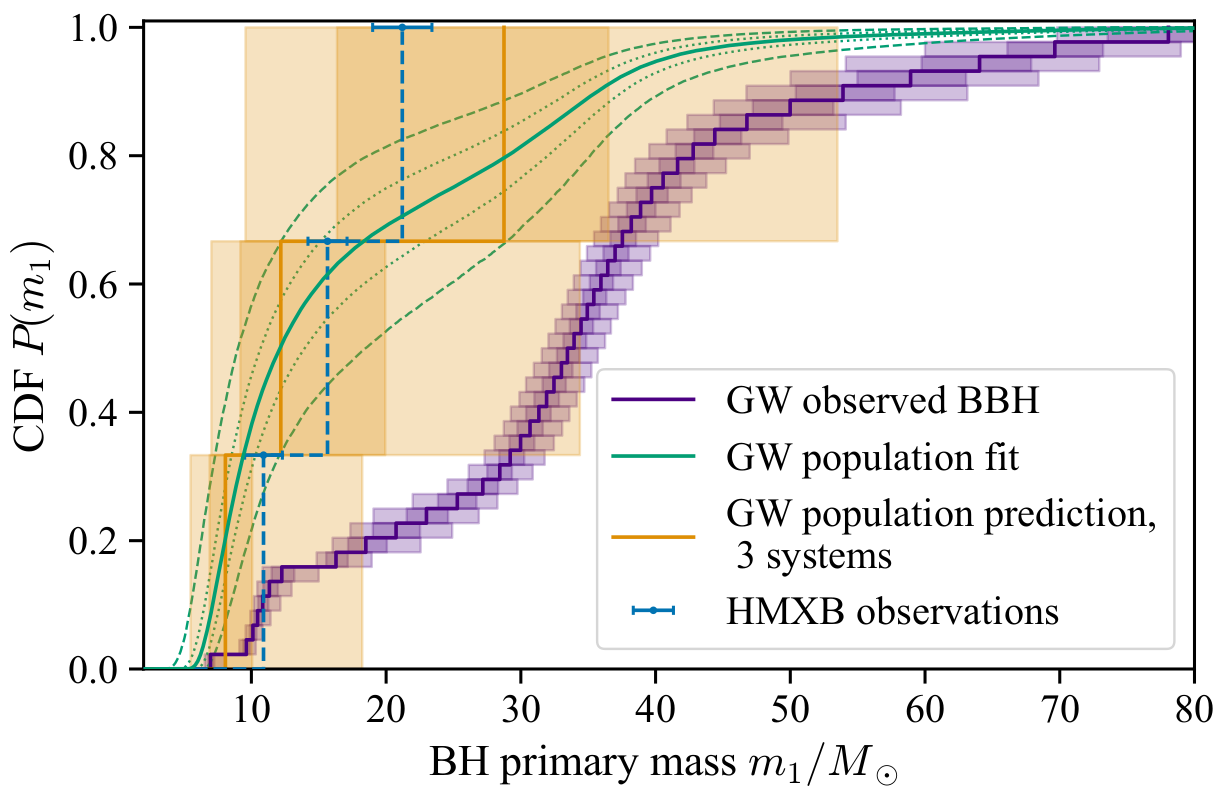
\includegraphics[width=\textwidth]{./images/tensionHMXBHmass.png}
	\end{minipage}
	\hfill
	\begin{minipage}{.49\textwidth}
		\vspace{.5mm}
		\centering
		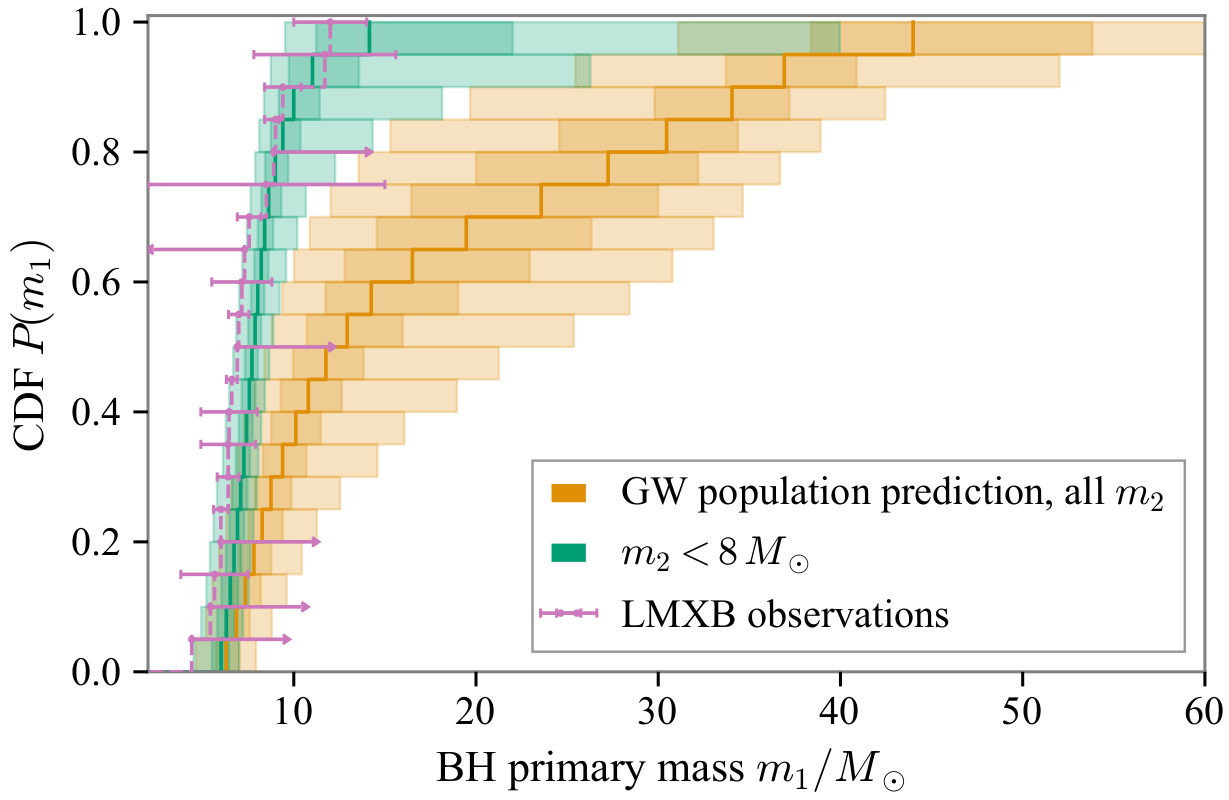
\includegraphics[width=\textwidth]{./images/tensionLMXBHmass.png}	
	\end{minipage}
	\caption{Observed cumulative distribution function (CDF) of the observed HMXBs (blue, \emph{left-hand} panel) and LMXBs (pink, \emph{right-hand} panel) compared with the CDFs (orange bands) expected if the X-ray binaries share the same primary black hole mass distribution as the primaries of the LVC binary black holes, once it is corrected for selection effects (green line). In the left-hand panel, the purple bands show the original observed CDF for binary black holes not yet corrected for observational effects. In the right-hand panel, the green bands show the CDF extracted from the sub-sample of the LVC binary black holes with secondary mass $< 8~\msun$. Dark (light) shaded areas delimit 50 \% (90 \%) credible intervals \cite{HMXBH_spins2021}}.\label{fig:tensionmass}
\end{figure}

\subsection{Similarities in the mass distribution}
The mass distribution of the primary (more massive) black hole of the LVC binary black holes seems compatible with the mass distribution of the black holes in LMXBs and HMXBs, once the corrections for gravitational wave selection effects and similar mass pairing are taken into account. If confirmed, the relation would indicate that X-ray binaries hosting a black hole could be the progenitors of the binary black hole mergers. However, the small sample of X-ray binaries with reliable mass measurements ($\sim 20$) is affected by a large Poisson uncertainty, possibly hiding inconsistencies in the underlying populations. Moreover, observational selection effects on the X-ray binaries are not accounted for and may further change the degree of consistency. \\

The left- and right-hand panel in Fig.\ \ref{fig:tensionmass} show the agreement between the cumulative distribution functions (CDF) of the primary black hole population underlying in the gravitational wave observations and the CDFs for the black hole population underlying in the HMXBs and LMXBs, respectively. The observed CDF of the 44 black hole primaries considered in the GWTC-2 (purple bands in the left-hand panel of Fig.\ \ref{fig:tensionmass}) is corrected for the observational selection effects that favour the detection of gravitational waves produced by heavy black holes (see Sec.\ \ref{subsec:GWtheorymethod}). The corrected posterior CDF (green line in the left-hand panel of Fig.\ \ref{fig:tensionmass}) is indeed shifted towards lower masses and describes the \textit{intrinsic} primary mass distribution of the black holes detected by the LVC. 

The observed CDFs of HMXBs and LMXBs (the blue and pink dashed lines in the left- and right-hand panels of Fig.\ \ref{fig:tensionmass}, respectively) cannot be directly compared with the intrinsic CDF of the primary black hole masses. The considered sample of HMXBs and LMXBs with \erika{reliable masses} contains, respectively, only 3 and 20 black holes: their CDFs are dominated by Poisson uncertainties if they are extracted from the same intrinsic population of binary black holes. To account for Poisson noise, many sets of 3 or 20 black holes are randomly extracted from the intrinsic binary black hole distribution (the green line already found). Each set is then used to build a CDF. Subsequently, all the extracted CDFs of 3 (20) black holes are put together to reconstruct a CDF representative of the black holes in HMXBs(LMXBs) than will become primary black holes in the binary black hole systems detected with gravitational waves (orange bands in both the panels of \ref{fig:tensionmass}). The extracted CDFs have very large credible intervals, as expected from the huge Poissonian noise acting on the limited sample of the X-ray binaries. \\

On the one hand, the left-hand panel of Fig.\ \ref{fig:tensionmass} shows that the observed mass distribution of black holes in HMXBs (blue) is compatible within 50 \% credible intervals with the distribution expected if the black holes of the HMXBs become the primaries of the LVC binary black holes (orange). On the other hand, the right-hand panel of Fig.\ \ref{fig:tensionmass} shows that LMXBs seem to have an observed black hole mass distribution (pink) too much shifted towards lower masses with respect to the one expected from being a progenitor of the LVC binary black holes (orange). However, the discrepancy is removed if the expected CDF is not extracted from all the 44 \erika{binary black holes} but only from the binaries with light secondary black holes $M_2 < 8~\msun$ (green bands). The selection of the sub-sample of binaries is justified because isolated binaries seems to favour the production of similar masses remnants and the LMXBs already host a low-mass secondary $\lesssim 2-3~\msun$. Even though secondary stars so light will unlikely produce black holes up to $8~\msun$, the agreement in the CDFs could suggest that possible differences in the LMXBs and binary black hole masses may be caused by the mass of the secondary star and not by the mass of the primary black hole \cite{HMXBH_spins2021}.



\begin{figure}
	\begin{minipage}{.49\textwidth}
		\centering
		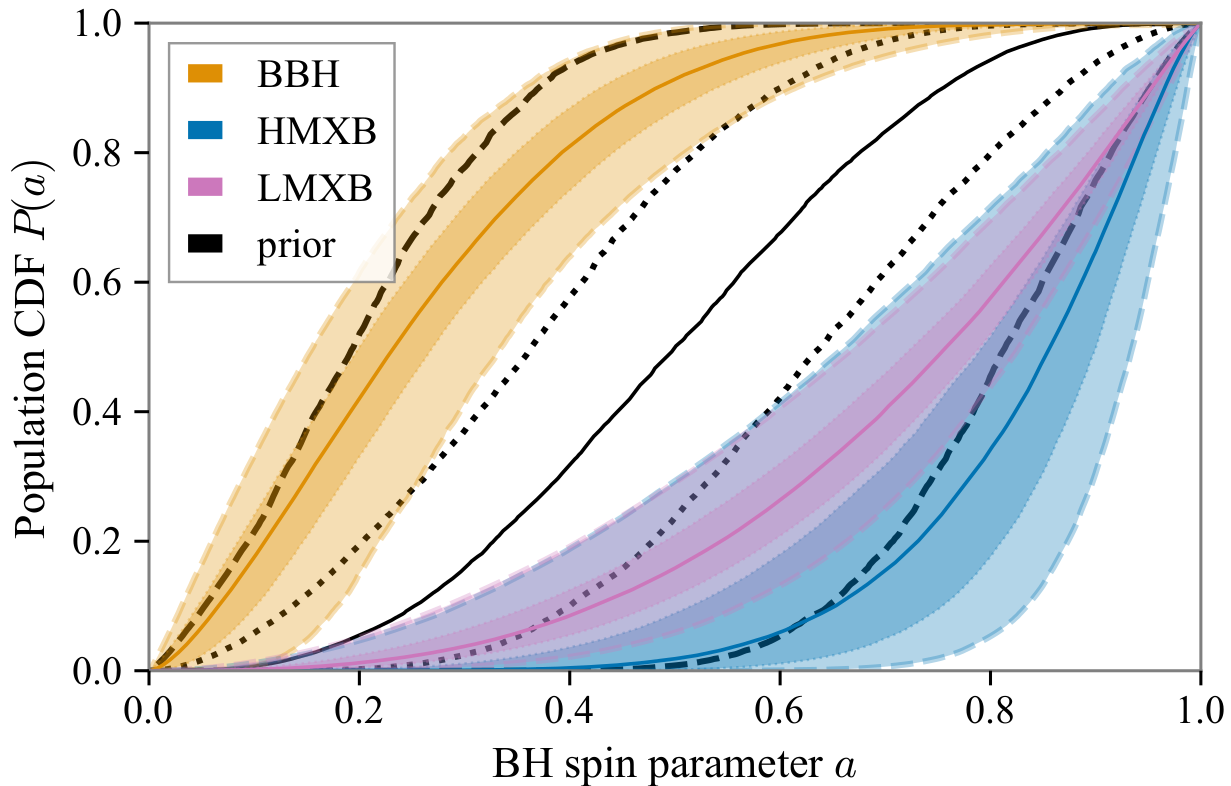
\includegraphics[width=\textwidth]{./images/tensionspin.png}
	\end{minipage}
	\hfill
	\begin{minipage}{.49\textwidth}
		\vspace{.5mm}
		\centering
		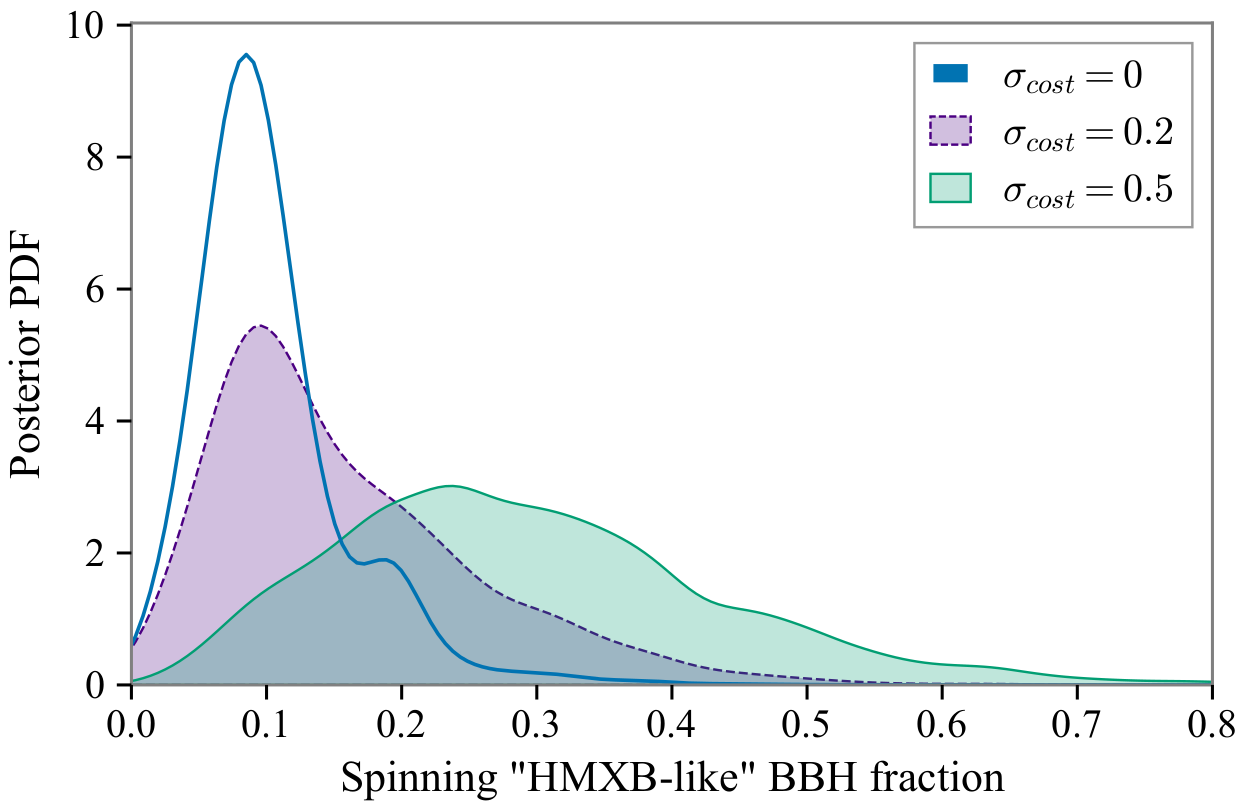
\includegraphics[width=\textwidth]{./images/tensionspinHMXBHlike.png}	
	\end{minipage}
	\caption{\emph{Left:} cumulative distribution function (CDF) of primary and secondary black hole spins detected with gravitational wave detectors in GWTC-2 (orange) compared with the ones of LMXBs (pink) and HMXBs (blue). The black lines show the prior beta distribution used for the fits. The spin distribution of the binary black holes is in tension with the ones inferred from the X-ray binaries. \emph{Right:} Posterior distributions of the fraction of binary black holes that could have evolved from a HMXB-like configuration. The more the primary spin is aligned to the orbital angular momentum (smaller $\sigma_{\rm \cos \theta}$ values, see Sec.\ \ref{subsec:tensionspin} for more detail) and the more the HMXB configuration is irrelevant in the underlying population \cite{HMXBH_spins2021}.}\label{fig:tensionspin}
\end{figure}


\subsection{Strong tension in the spin distribution}\label{subsec:tensionspin}
The spin distribution of the black holes detected with the gravitational waves (including both primary and secondary black holes) seems to be in tension with the spin distribution of the black holes detected in X-ray binaries, as visible in the left-hand panel of Fig.\ \ref{fig:tensionspin}. The LVC binary black holes appear to host slowly spinning black holes, whereas both the LMXBs and HMXBs contain fast rotating black holes. Beta distribution fits to the observed spins of the LMXBs (pink) and HMXBs (blue) denote that the two types of X-ray binaries have spin distributions consistent within 90~\%. A single beta distribution fitted to the LMXBs and HMXBs altogether exhibits a disagreement at the 99.9~\% level with the spin distribution of the LVC binary black holes (orange).\cite{HMXBH_spins2021}\\

The three HMXBs considered here (LMC X-1, M33 X-7 and Cyg X-1) host very fast spinning black holes $\chi \gtrsim 0.8$: if they produce a binary black hole in the isolated binary evolution scenario, it is likely that mass transfer and tidal locking will align the spins to the orbital angular momentum of the binary \cite{Kalogera2000_spinaligned}. Nevertheless, supernova kicks may still cause a tilt in the spin orientation. \erika{Overall, the toy model usually adopted for the tilt angles $\theta$ is a half-Gaussian in $\cos \theta$, peaked at aligned spins $\cos \theta = 1$  with some standard deviation $\sigma_{\rm \cos \theta}$: the larger the tilt angle, the larger the standard deviation} \cite{spintiltmodel_Talbot2017}. % so che è un toy model ma devo comunque introdurlo perché è il toy model usato da fishbach e kalogera, i cui parametri compaiono nei grafici che mostro

It is possible that a sub-population of binary black holes has evolved through a HMXB-like configuration; Bayesian inference methods can be used to put upper limits to the fraction of binary black holes belonging to it. One of the input parameters of the inference method is the effective spin $\chi_{eff}$ i.\ e.\ the mass-weighted component of the spins aligned to the orbital angular momentum (see Eq.\ \ref{eq:chieff}). Determining the upper limits in the sub-population weight means assuming that the $\chi_{eff}$ is mainly determined by the spin of the primary black hole. Therefore, a black hole binary coming from a HMXB-like configuration will be modeled with secondary spin narrowly peak around zero and primary spin distributed with the half-Gaussian in $\cos \theta$. 

The right-hand panel in Fig.\ \ref{fig:tensionspin} shows the results of three possible estimates of the sub-population weight allowing for three different maximum tilts of the primary spin: no tilt ($\sigma_{\rm \cos \theta} = 0$), $\lesssim 12^{\circ}$ tilt ($\sigma_{\rm \cos \theta} = 0.2$) or $\lesssim 30^{\circ}$ tilt ($\sigma_{\rm \cos \theta} = 0.5$). The more the primary spin is forced to be aligned, the less the HMXB configuration is relevant in the formation history of the binary black hole. The fraction of binaries belonging to the sub-population of HMXB-like binaries is only $< 19 \% $ for aligned spins, growing to $< 30 \%$ for slightly tilted spins ($\sigma_{\rm \cos \theta} = 0.2$) and up to $< 48 \%$ for mildly tilted spins ($\sigma_{\rm \cos \theta} = 0.5$).\\

The evolutionary mechanisms necessary to create a rapidly spinning primary in a system that forms a binary black hole merging within a Hubble time are still under investigations. One of the proposed channels involves a stable mass transfer event from a main sequence donor to a main sequence accretor. If the angular momentum transport is inefficient inside the star and the mass transfer can remove its envelope tidally-locking the system, a lot of the angular momentum can be maintained in the core of the donor star. After a similar mass transfer, the donor will rapidly become a Wolf-Rayet star and eventually produce a fast spinning black hole \cite{spinfastBH_Qin2019}. Population synthesis studies coupled with detailed stellar evolution models showed that only $\lesssim 12 \%$ of the HMXB binaries formed in this way had the right combination of parameters to evolve into a black hole binary that merges via gravitational wave emission within a Hubble time. Overall, only $\lesssim 20 \%$ of the merging \erika{binary black holes} seem to undergo this kind of evolution, in agreement with the upper limit of $\lesssim 30 \%$ found for slightly tilted spins \cite{HMXBHspins2022}.





\chapter{Wolf-Rayet -- black hole binaries}
\paragraph{An intermediate evolutionary stage}
The systems composed of two massive stars are the best possible progenitors for the LVC binary black holes, if the stars are massive enough to form a black hole ($\mzams \gtrsim 15-25~\msun$ at solar metallicity, according to single stellar evolution \cite{Limongi2017_handbookSN}) and if their orbit is tight enough to undergo at least one mass transfer episode: 82 O-type stars with mass $\sim 15-60~\msun$ observed in six Galactic open clusters revealed that $70 \%$ of the massive stars are born in binaries, close enough to allow mass transfer interaction \cite{Sana2012}. 

Population-synthesis studies suggest that at least one mass transfer episode is necessary to shrink the orbit and allow the coalescence within a Hubble time \cite{spera2019_mergingBBH}. On the one hand, it is difficult to predict the type of mass transfer and the fate of the binary because they strongly depend on the orbital separation and on stellar evolution details, as shown in Fig.\ \ref{fig:Sana2012MTfate}. On the other hand, usually the mass transfer and the strong stellar winds strip the hydrogen envelope of massive stars, producing a Wolf-Rayet star. If the right conditions are met, the binary system evolves until it becomes a black hole -- Wolf-Rayet star system: the strong winds of the Wolf-Rayet star can power the accretion disk of the black hole and make the system visible as an X-ray binary.

\paragraph{Chapter outline}
This chapter reviews the theory of single stellar evolution and the main mass transfer processes (wind-fed accretion, Roche lobe overflow and common envelope) to better understand the evolution of Wolf-Rayet -- black hole binaries. I will report the observed properties of the known Wolf-Rayet -- black hole systems, discussing the main issues in parameter estimation. Finally, I will describe the Cyg X-3 system: the only known Galactic Wolf-Rayet -- black hole binary.


\begin{figure}[h!]
	\centering
	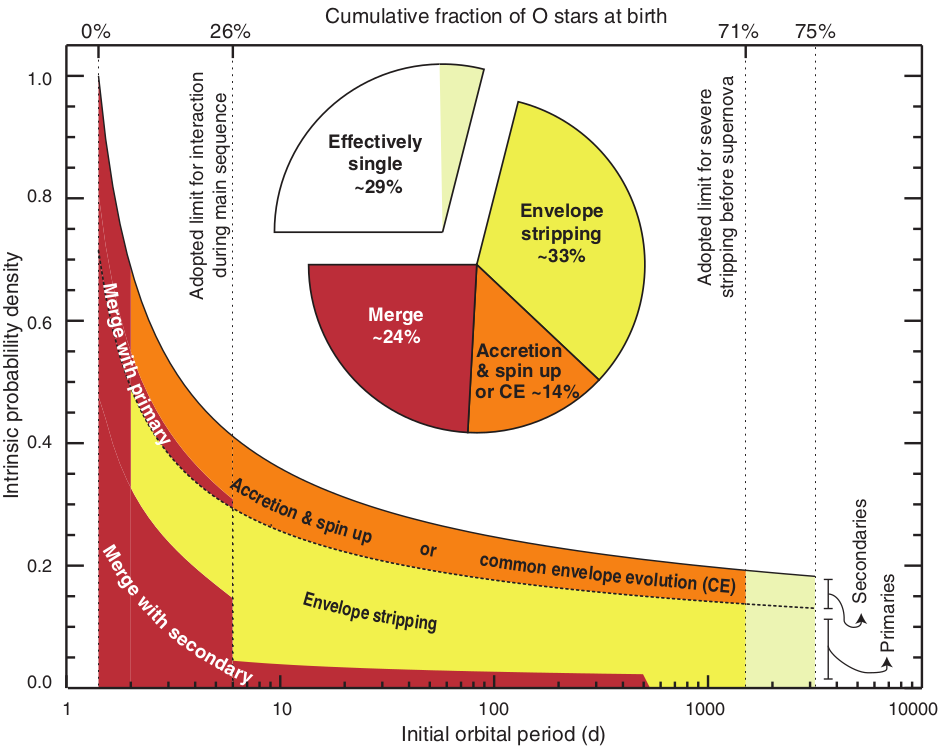
\includegraphics[width=.65\textwidth]{./images/Sana2012MTfate.png}
	\caption{70\% of O-type stars will be part of a binary with initial period $< 1500$ days and will undergo at least one mass transfer process. The type of mass transfer and the fate of the binary will depend on the details of single stellar evolution and on the orbital separation \cite{Sana2012}.}\label{fig:Sana2012MTfate}
\end{figure}



\section{Wolf - Rayet stars}
\subsection{Spectral classification of a Wolf-Rayet star}\label{subsec:WRclassification}
\paragraph{Peculiar properties} Wolf-Rayet (WR) stars are named after the French astronomers Charles Wolf and Georges Rayet that in 1867 first discovered three stars in the Cygnus constellation with strong and broad emission lines. More than a century after, a few hundreds of Wolf-Rayet stars were discovered in the Milky Way, $\sim 40 \%$ of which are part of binary systems.

Stellar spectra usually exhibit a continuum with narrow absorption lines. Generally, the hot radiation coming from the interior is absorbed by atoms and molecules in a cooler stellar photosphere ($T_{\rm eff} \lesssim 60 000$ K in the hotter O-type stars). In contrast, the photosphere of Wolf-Rayet stars is much hotter ($T_{\rm eff} \sim 60~000 - 100~000$ K) and hosts many heavy elements, often ionized (like He, N, C or O). The atoms and ions in the photosphere strongly interact with the energetic photons coming from the interior: they produce recombination and fluorescence emission lines (visible in the UV, optical and near-IR bands) while efficiently absorbing the momentum of photons via multiple-scatterings. The net effect is the production of a very dense and strong wind ($\mdot \sim 10^{-4}-10^{-5}~\msun~\yr^{-1}$) with broad emission lines of elements and ions usually absent in other stellar spectra.

\paragraph{Classification and evolutionary sequence}The spectrum of Wolf-Rayet stars is their distinctive feature and is used to classify them on the basis of the presence and abundance of peculiar elements in the photosphere. The most important lines adopted for the classification are reported in Tab.\ \ref{tab:WRclassification} and characterize the three sub-types: WN (strong lines of helium and nitrogen), WC (strong lines of helium, carbon and less prominent lines of oxygen) and WO (strong lines of oxygen and less prominent lines of helium and carbon). The WN stars can be further divided into two subfamilies on the basis of their surface hydrogen abundance $X_H$: WNL (late) if $X_H \gtrsim 0.5$ or WNE (early) if $X_H \lesssim 0.5$. In contrast, WC and WO stars lack hydrogen lines: it is probable that they lost the external envelope because of stellar winds or as a result of mass transfer.  

The helium, nitrogen, carbon and oxygen detected in the photosphere were produced by the CNO cycle and triple-$\alpha$ reactions of H- and He-burning, respectively. Usually these elements can reach the photosphere only as a result of dredge-up events, but their abundance is lower than the one detected in Wolf-Rayet stars. Recalling that the hydrogen envelope is either small or depleted, it is likely that the observed types of Wolf-Rayet stars are part of an evolutionary sequence of massive stars: the external layers are progressively removed and expose the more metal-rich ones. According to this interpretation, the evolution would proceed as

\[\rm WNL \rightarrow WNE \rightarrow WC \rightarrow WO\]

\paragraph{Type II and Ib/c supernovae} Wolf-Rayet stars that explode with little (WN) or no hydrogen envelopes (WC,WO) are likely the progenitors of, respectively, the Type II and Type Ib/Ic core-collapse supernovae. The stronger hints come from the observations of supernova light curves: Type II supernovae exhibit hydrogen lines, Type Ib lack hydrogen but exhibit He and Type Ic lack both hydrogen and helium \cite{WR_signature,parsec2015_chen,Limongi2010_preSNevo}.

%pluto some lines may still need to be added but for the rest is ok
\renewcommand{\arraystretch}{1.5}
\begin{figure}[h]
	\centering
		\begin{tabular}{lll}
			\toprule
			WR type & Elements & Wavelength $\lambda$ of the strongest lines \\
			\midrule
			\multirow{2}{*}{WN}  & He I-II  & 2.058 $\mu\rm m$~[He I]; 1640 \AA , 4686 \AA, 5412 \AA, 1.012 $\mu\rm m$, 2.189 $\mu\rm m$~[He II]  \\
			& N III-V & \\ 
			\hline
			\multirow{2}{*}{WC}  & C III-IV  & 4650 \AA, 5696 \AA ~[C III]; 1550 \AA,  5548-51 \AA, 5801-12 \AA, 2.08 $\mu\rm m$~[C IV] \\
			& O III-V & \\
			\hline
			\multirow{2}{*}{WO}  & C IV  &\\
			& O V-VI & 3811-34 \AA~[O VI]\\
			\bottomrule 	
		\end{tabular}
		\captionof{table}{Main UV, optical and near-IR emission lines used for the spectral classification of Wolf-Rayet stars \cite{WR_signature, CygX-3_Koljonen2017}} \label{tab:WRclassification}
\end{figure}



\subsection{Mass determination of a Wolf-Rayet star}\label{subsec:massWR}
\paragraph{Dynamical masses} The mass of the Wolf-Rayet stars that are member of a binary system with a non-degenerate companion can be determined with the dynamical method described in Sec.\ \ref{subsec:Xraymeasure}. The largest uncertainties come from binary inclination, thus, observations in eclipsing binaries (for which the edge-on orientation better constraints the inclination) allow the most precise mass determinations. Dynamical measurements revealed that WC stars are lighter than the WN ones, supporting the evolutionary sequence of Wolf-Rayet stars described in Sec. \ref{subsec:WRclassification}: WC are limited to $\rm M_{\rm WC}\sim 9-16~\msun$ while WN extend to $\rm M_{\rm WN}\sim 10-83~\msun$ \cite{WR_signature}.

\paragraph{Isolated Wolf-Rayet stars and Wolf-Rayet stars with a degenerate companion} The dynamical method cannot be used for stars with a degenerate companion (like a neutron star or a black hole) or for the isolated ones. Furthermore, the dense stellar wind of Wolf-Rayet stars prohibits reliable measurements of the surface gravity from the photospheric lines. 

The only method left relies on the theory of stellar evolution.  Detailed calculations can relate the mass of a star in a given evolutionary stage to its expected observable properties, including its luminosity. If the distance and age of the Wolf-Rayet star are known (for instance for  Wolf-Rayet stars in star clusters), it is possible to reconstruct its intrinsic luminosity. Thus, to determine the mass of an isolated Wolf-Rayet star it is sufficient to measure its luminosity and adopt a mass-luminosity relation obtained from theoretical calculations. It is important to note that the mass-luminosity relations strongly depend on stellar evolution assumptions and need to be carefully calibrated, for instance with Wolf-Rayet stars in binary systems whose mass is already known from dynamics \cite{Nugis2000_WRwinds}.

\paragraph{Upper mass-luminosity relation} The luminosity of a star depends on the nuclear reactions acting in the core of the star and, thus, on the chemical composition. In general, stars that are not chemically-homogeneous and have a mean molecular weight higher in the core and lighter in the surface. However, considering a homogeneous star allows to put an upper limit on the mass related to a given luminosity: if the core is lighter (because of the chemical homogeneity imposed) more mass is required to produce the same luminosity. 

The left-hand panel of Fig.\ \ref{fig:MLandwinds} shows the quadratic dependence of the luminosity on the mass of chemically-homogeneous stars. The same massive star is more luminous if the core is heavier, with a linear dependence of the luminosity on the hydrogen abundance $X_H$: the less the hydrogen content in the large convective core, the higher the mean molecular weight, thus, the higher the surface luminosity \cite{Grafener2011_M-L_WR}.
 
 
\begin{figure}[h]
	\begin{minipage}{.49\textwidth}
		\centering
		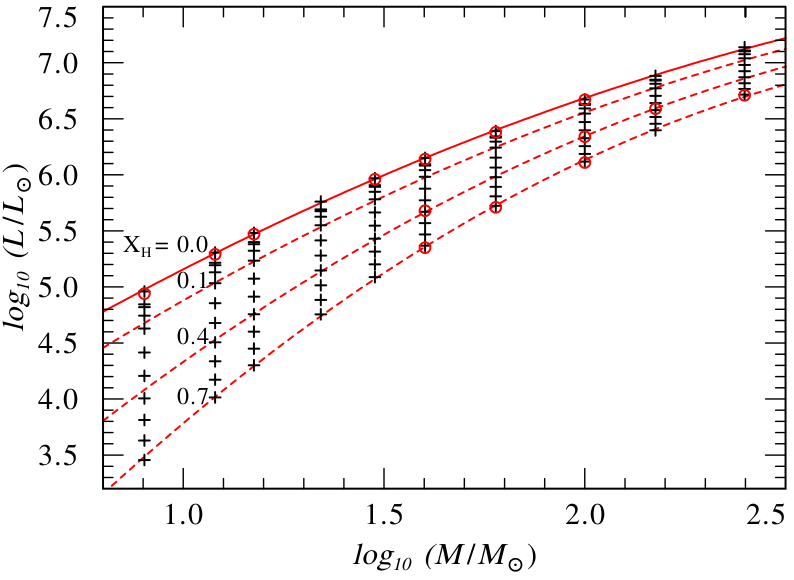
\includegraphics[width=.94\textwidth]{./images/MLrelation.png}
	\end{minipage}
	\hfill
	\begin{minipage}{.49\textwidth}
		\centering
		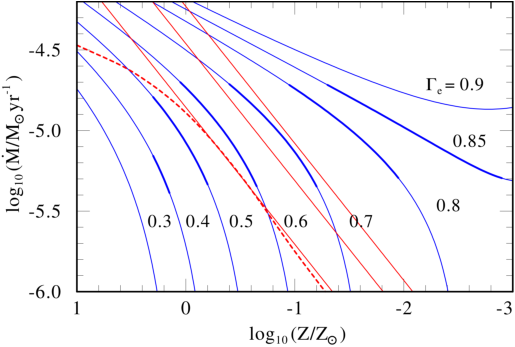
\includegraphics[width=\textwidth]{./images/stellarwinds.pdf}	
	\end{minipage}
	\caption{\emph{Left:} Mass-luminosity relations for chemically-homogeneous massive stars with fixed hydrogen abundance $X_H$. The black crosses indicate the computed stellar models, the dashed red lines the fits for hydrogen-core burning stars with different $X_H$, the solid red line indicates pure-Helium stars ($X_H = 0$) burning helium in their cores \cite{Grafener2011_M-L_WR}. \emph{Right:} Mass loss rates dependent only on the metallicity as in Vink et al.\ 2001 \cite{Vink2001} (red solid lines) or also on the Eddington factor as in Gr{\"a}fener \& Hamann 2008 \cite{G&H_WRmassloss} (blue solid lines). The simplified model of Vink et al.\ 2001 strongly underestimates the mass lost by low-metallicity stars close to the Eddington limit $\Gamma_e \sim 1$. The red dashed line indicates a model not considered in this thesis \cite{G&H_WRmassloss}.}\label{fig:MLandwinds}
\end{figure}

\subsection{Stellar winds of the massive stars}\label{subsec:stellarwinds}
\paragraph{Metallicity dependence} O,B and Wolf-Rayet stars are massive and hot stars with $\rm T_{\rm eff} \gtrsim 12~000$ K that emit the bulk of photons in the UV regime and suffer \emph{line-driven winds}. The radiation coming from the star interior is so energetic that ionizes the atoms of C, N, O, Ne, Si, S in the photosphere. The absorption lines of the ions, especially of the ones of the C IV, are precisely in the UV regime: photons impinging on the ions are absorbed and their momentum is transferred. The accelerated ions share their momentum via Coulomb interactions with nearby nuclei and electrons, with the net effect of accelerating the whole gas. Intuitively, the higher the temperature and the metal content and the more a larger number of ions can be produced and absorb the momentum of the photons, increasing the amount of mass lost.\\

In 2001, Vink et. al.\ \cite{Vink2001} carried out Montecarlo simulations on a grid of 540 models of O and B Main Sequence stars, quantifying the dependence of the mass loss rate $\mdot$ on the metallicity $Z$ and effective temperature $\rm T_{\rm eff}$ as

\begin{equation}\label{eq:Vink2001}
\dot{M} \propto Z^{0.85}~v_\infty^p \quad \quad p = 
\begin{cases}
-1.23 & T_\textup{eff} \gtrsim \SI{25 000}{K} \\
-1.60 & \SI{12 000}{K} \lesssim T_\textup{eff} \lesssim \SI{25 000}{K}
\end{cases}
\end{equation}

where $v_\infty$ is the terminal velocity of the wind, reached when the gas is far enough from the star that is no more accelerated by the radiation field. The mass loss rate depends also on the stellar mass and luminosity; although with slightly different exponents for the different temperature ranges, the order-of-magnitude dependence is $\mdot \propto L^{2.2} M^{-1.3}$. \\

Wolf-Rayet stars have a metal-enhanced composition on their surface, suggesting a mass loss rates dependence on both the mass fraction of the metals heavier than He ($Z$)and on the one of the helium alone ($Y$). In 2000, Nugis \& Lamers \cite{Nugis2000_WRwinds} observed 34 WN and 30 WC stars in the Milky Way, quantifying the dependence as

\begin{equation}\label{eq:NugisLamers2000}
	\mdot \sim 1.0 \times 10^{-11}~(L/L_\odot)^{1.29}~Y^{1.7}~Z^{0.5}
\end{equation}

\paragraph{Eddington factor dependence}
Hot stars like the O,B and the Wolf-Rayet have radiative external envelopes: the radiation pressure of the energetic photons produced in the core pushes on the free electrons, that interact via Thomson scattering and efficiently transport the energy outwards. However, the radiation pressure can be so strong to overcome the self-gravity of the star: the external layers are no more in hydrostatic equilibrium and are pushed away. The mass expelled changes the observed luminosity and the star becomes a variable; a Luminous Blue Variable (LBV) if the original stars were of the O or B types.

Assuming that the pressure gradient of the star is due only to the Thomson scattering, the self-gravity of the star cannot support the hydrostatic equilibrium if the luminosity $L$ exceeds the Eddington one $L_{\rm Edd}$. The maximum permitted luminosity $L=L_{\rm Edd}$ defines the \emph{Eddington limit} $\Gamma_e$

\begin{equation}\label{eq:Eddingtonfactor}
\Gamma_e = \frac{L}{L_\textup{Edd}} = \frac{L k_\textup{es}}{4 \pi c G M}
\end{equation}

The Eddington factor for a fully ionized plasma is given by

\begin{equation}\label{eq:EddingtonObserved}
\Gamma_e = 10^{-4.813}~(1+X_H)~(L/L_\odot)~(M_\odot/M)
\end{equation}

The surface abundance of hydrogen $X_H$ is known from spectroscopic observations. Measuring the intrinsic luminosity and adopting the mass-luminosity relations, as described in Sec.\ \ref{subsec:massWR}, it is possible to recover the Eddington factor of the observed stars.\\


Stars that approach and overcome the Eddington limit $\Gamma_e \geq 1$ have enhanced mass losses and are likely the progenitors of the Wolf-Rayet stars, as discussed in Sec.\ \ref{subsec:stellarevo}. The evolution close to the Eddington limit, coupled with multiple scatterings in the winds, can explain the strong stellar winds of the Wolf-Rayets. In 2008, Gr{\"a}fener \& Hamann \cite{G&H_WRmassloss} used detailed and self-consistent modeling of non-LTE atmospheres and winds of WNL stars to compute the expected mass loss rates. A rough fit \cite{parsec2015_chen} to their relations underlines a continuity to the 2001 models of Vink et al.\

\begin{equation}\label{eq:WRwindGH2008}
\dot M \propto Z^{\alpha} \quad \quad  \alpha = 
\begin{cases}
0.85 & \Gamma_e < 2/3 \\
2.45-2.4~\Gamma_e & 2/3 \leq \Gamma_e \leq 1
\end{cases}
\end{equation}

Gr{\"a}fener \& Hamann found that the metallicity-dependence of Eq.\ \ref{eq:Vink2001} is enhanced for stars closer to the Eddington limit. As shown in the right-hand panel of Fig \ref{fig:MLandwinds}, not accounting for the dependence on $\Gamma_e$ results in a severe underestimation of the mass loss rates, especially at lower metallicities.\\

Vink et al.\ in 2011 \cite{Vink2011} re-calculated the mass loss rates on models of massive and very massive stars ($40-300~\msun$) including a dependence on the Eddington factor, finding

\begin{equation}\label{eq:Vink2011}
\begin{cases}
\dot M \propto M^{0.68}\ \Gamma_e^{2.2} & 0.4 \lesssim \Gamma_e \lesssim 0.7 \\
\dot M \propto M^{0.78}\ \Gamma_e^{4.77} & \Gamma_e \gtrsim 0.7
\end{cases}
\end{equation}





\subsection{Evolution of a massive star into a Wolf-Rayet}\label{subsec:stellarevo}

In this section I will discuss the evolution of the massive stars with particular attention to the conditions that favor the creation of Wolf-Rayet stars. I considered only stars with initial masses $\mzams \geq 20~\msun$, massive enough to likely produce a black hole in place of a neutron star after the core-collapse supernova (see Sec.\ \ref{subsec:SNmodels}), and with $\mzams \leq 100~\msun$, to avoid the discussion of the pair-instability supernovae that form at $Z=0.002$: the work of this thesis only focuses at solar metallicity $Z\sim 0.02$ where this phenomenon is not relevant \cite{spera2017_pisnSNe}. I will refer to the evolutionary tracks shown in Fig.\ \ref{fig:HRdiagrams} and \ref{fig:masslostWR} that I generated with the population-synthesis code \texttt{SEVN} \cite{spera2019_mergingBBH} interpolating the output tables of the \texttt{PARSEC} stellar evolution code \cite{parsec2015_chen} (further details in Sec.\ \ref{sec:SEVN}). The scope of this section is to provide a self-consistent reference to the work carried out in this thesis and presented in Sec.\ \ref{sec:results}. 

\paragraph{Wolf-Rayet stars with \texttt{PARSEC} and \texttt{SEVN}} The stellar winds implemented by \texttt{PARSEC} on the massive stars account both for the dependence on the metallicity and on the Eddington factor (see Sec.\ \ref{subsec:stellarwinds} for more details). In particular, the mass loss rates of the Blue Super Giants (BSG) and LBVs follow Vink et al.\ 2001 and Gr{\"a}fener \& Hamann 2008 (Eq.\ \ref{eq:WRwindGH2008}) while the ones of the Wolf-Rayets are based on the work of Nugis \& Lamers in 2000 (Eq.\ \ref{eq:NugisLamers2000}).\\

On the one hand, \texttt{PARSEC} classifies the Wolf-Rayet sub-types WNL,WNE and WC according to the surface abundance of many elements (hydrogen, helium, carbon, nitrogen, oxygen and iron) at different metallicities. For instance, at solar metallicity, the hydrogen fraction of WNL is $X_{\rm WNL} \leq 0.2$ while WNE and WC are consistent with no hydrogen $X_{\rm WNE} = X_{\rm WC} = 0$. On the other hand, \texttt{SEVN} considers a star as a Wolf-Rayet imposing a condition \emph{only} on the hydrogen fraction, requiring that $X_H \leq 0.2$. Stars with so little hydrogen on the surface are interpolated with different evolutionary tables: the stars are considered as pure-Helium and are computed starting from a helium Zero Age Main Sequence (He-ZAMS), obtained removing the hydrogen envelope to a normal star at the beginning of the core-He burning phase. The He-ZAMS stars then evolve following the same prescriptions of the normal stars \cite{spera2019_mergingBBH}.\\

It is important to point out that in this work the minimum masses needed to produce the Wolf-Rayet stars are higher with respect to other known works in the literature, for instance when compared to the ones obtained from the \texttt{FRANEC} stellar evolution code \cite{Limongi2010_preSNevo}. The main differences are in the amount of overshooting for the convective core\footnote{According to the mixing-length-theory, the mean free path $l_c = \Lambda_c H_p$ of the convective bubbles that overshoot into the upper radiative envelope can be parameterize as a fraction $\Lambda_c$ of the pressure scale height $H_p$ \cite{parsec2015_chen}.} in the central H-burning phase (0.2 $H_p$ in \texttt{FRANEC} and 0.5 $H_p$ in \texttt{PARSEC}) and in the threshold to classify a star as a Wolf-Rayet ($X_H \leq 0.4$ in \texttt{FRANEC} and $X_H \leq 0.2$ in \texttt{PARSEC} when interpolated with \texttt{SEVN}). Given that the Wolf-Rayets evolve with increased depletion of the hydrogen envelope, the $X_H \leq 0.4$ condition in \texttt{FRANEC} allows to form Wolf-Rayet stars earlier than in the \texttt{PARSEC} tracks interpolated by \texttt{SEVN}. In particular, \texttt{FRANEC} lowers the minimum initial mass required to form a Wolf-Rayet at solar metallicity to $\mzams \sim 30~\msun$, while the \texttt{PARSEC} tables interpolated by \texttt{SEVN} require a minimum mass of $\mzams \sim 40~\msun$. 




\begin{figure}[h!]
	\begin{minipage}{.49\textwidth}
		\centering
		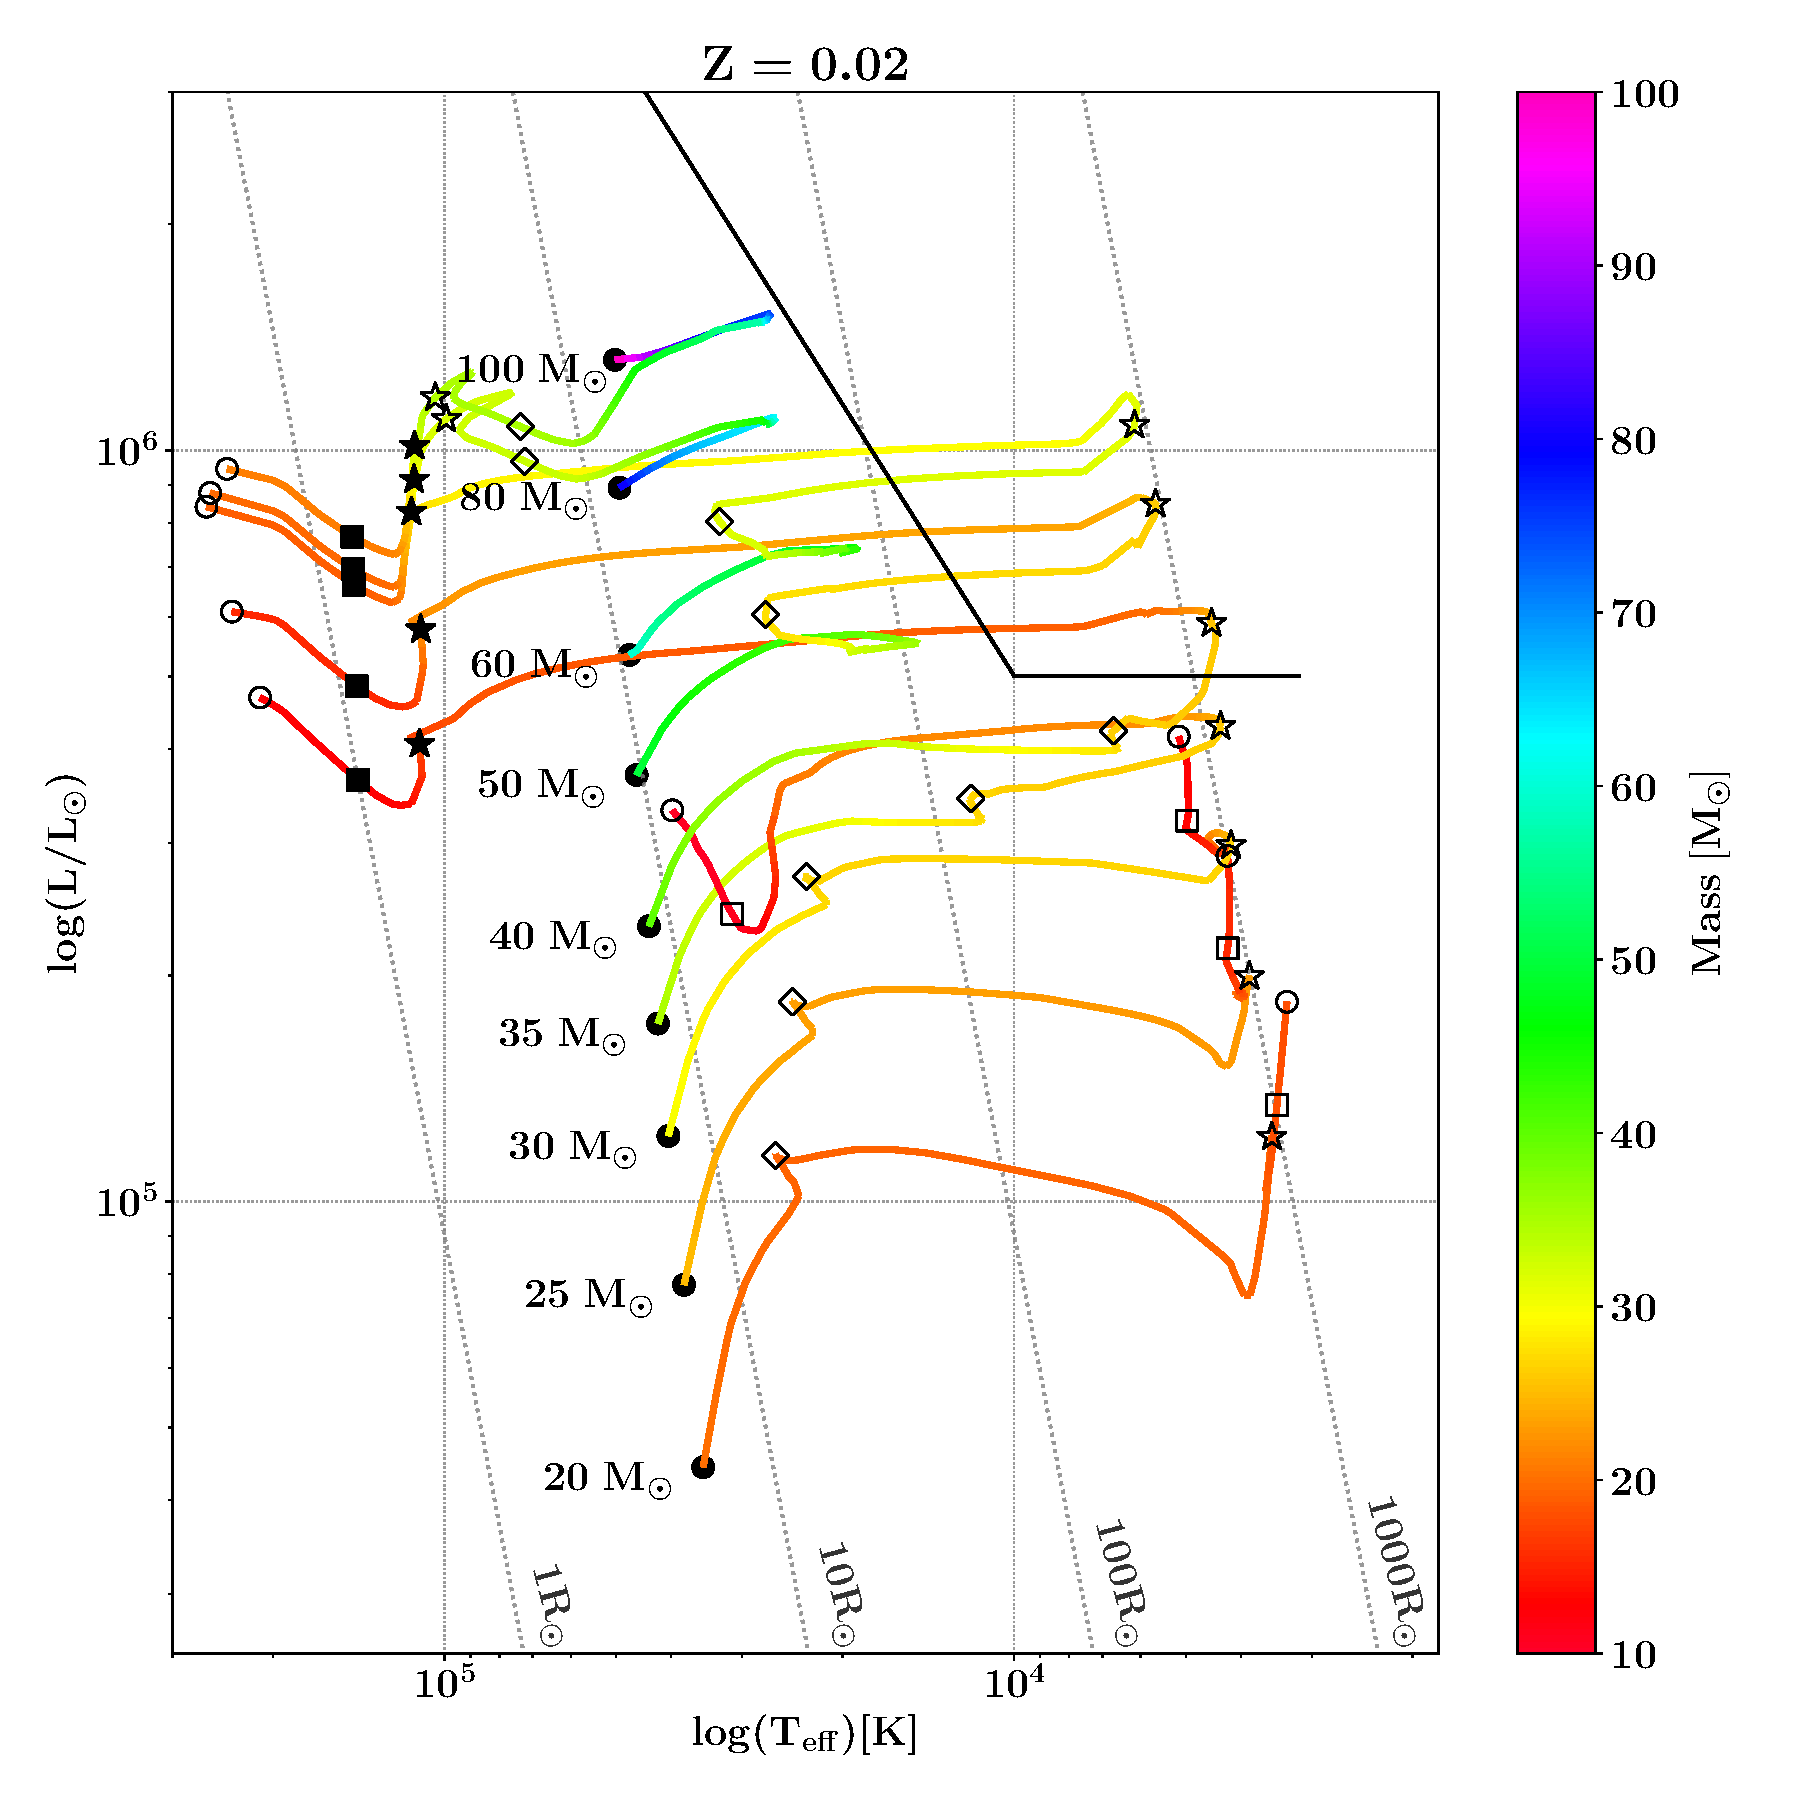
\includegraphics[width=1.05\textwidth]{./images/HR_02.pdf}
	\end{minipage}
	\hfill
	\begin{minipage}{.49\textwidth}
		\centering
		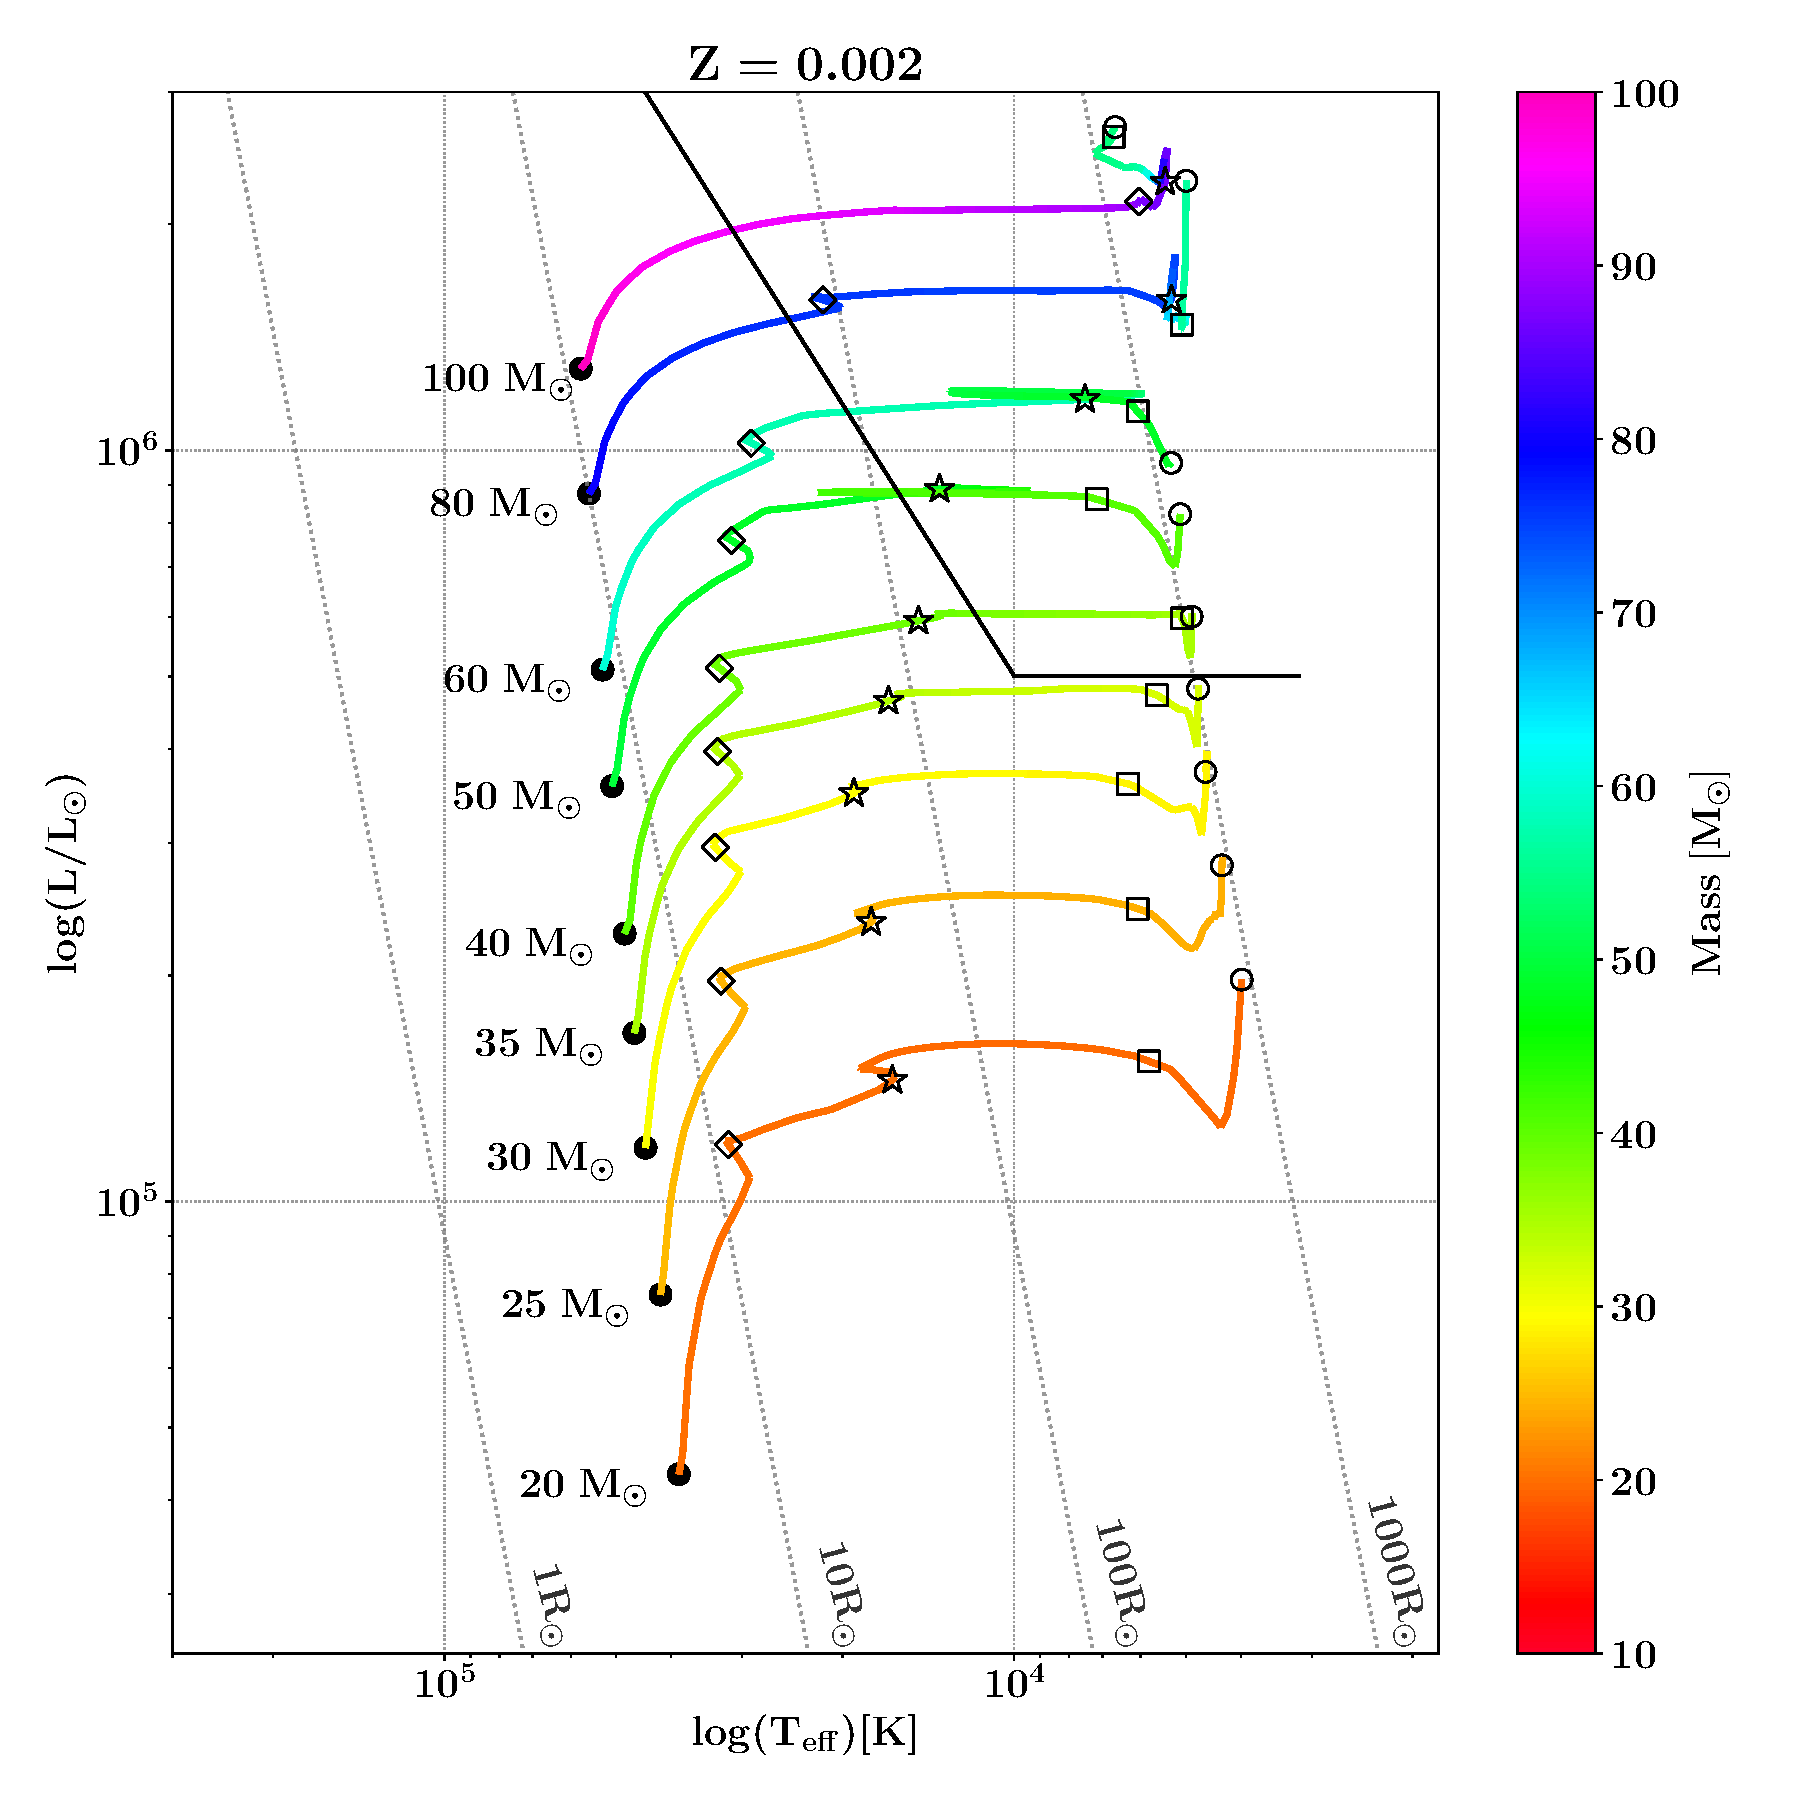
\includegraphics[width=1.05\textwidth]{./images/HR_002.pdf}	
	\end{minipage}
	\caption{Hertzsprung-Russel diagrams with the single stellar evolution of massive stars at two different metallicities. The symbols indicate the different burning stages: beginning of core H burning i.\ e.\ ZAMS (filled circle), beginning of H shell burning (empty diamond), beginning of the core He burning (empty star) possibly as a Wolf-Rayet (filled star), beginning of He shell burning (empty square) possibly as a Wolf-Rayet (filled square), end of the CO burning (empty circle). At solar metallicity ($Z=0.02$, \emph{left} panel) Wolf-Rayet stars can be produced by stars with $\mzams \gtrsim 40~\msun$ while at metallicity one order-of-magnitude lower ($Z=0.002$, \emph{right} panel) the stellar winds are quenched and even stars with $\mzams \sim 100~\msun$ can't produce a Wolf-Rayet. I generated the tracks with the population-synthesis code \texttt{SEVN} \cite{spera2019_mergingBBH}, that interpolates the tables produced with the \texttt{PARSEC} stellar evolution code \cite{parsec2015_chen} (more details on the codes in Sec.\ \ref{sec:SEVN}).}\label{fig:HRdiagrams}
\end{figure}


\begin{figure}[h!]
	\begin{minipage}{.49\textwidth}
		\centering
		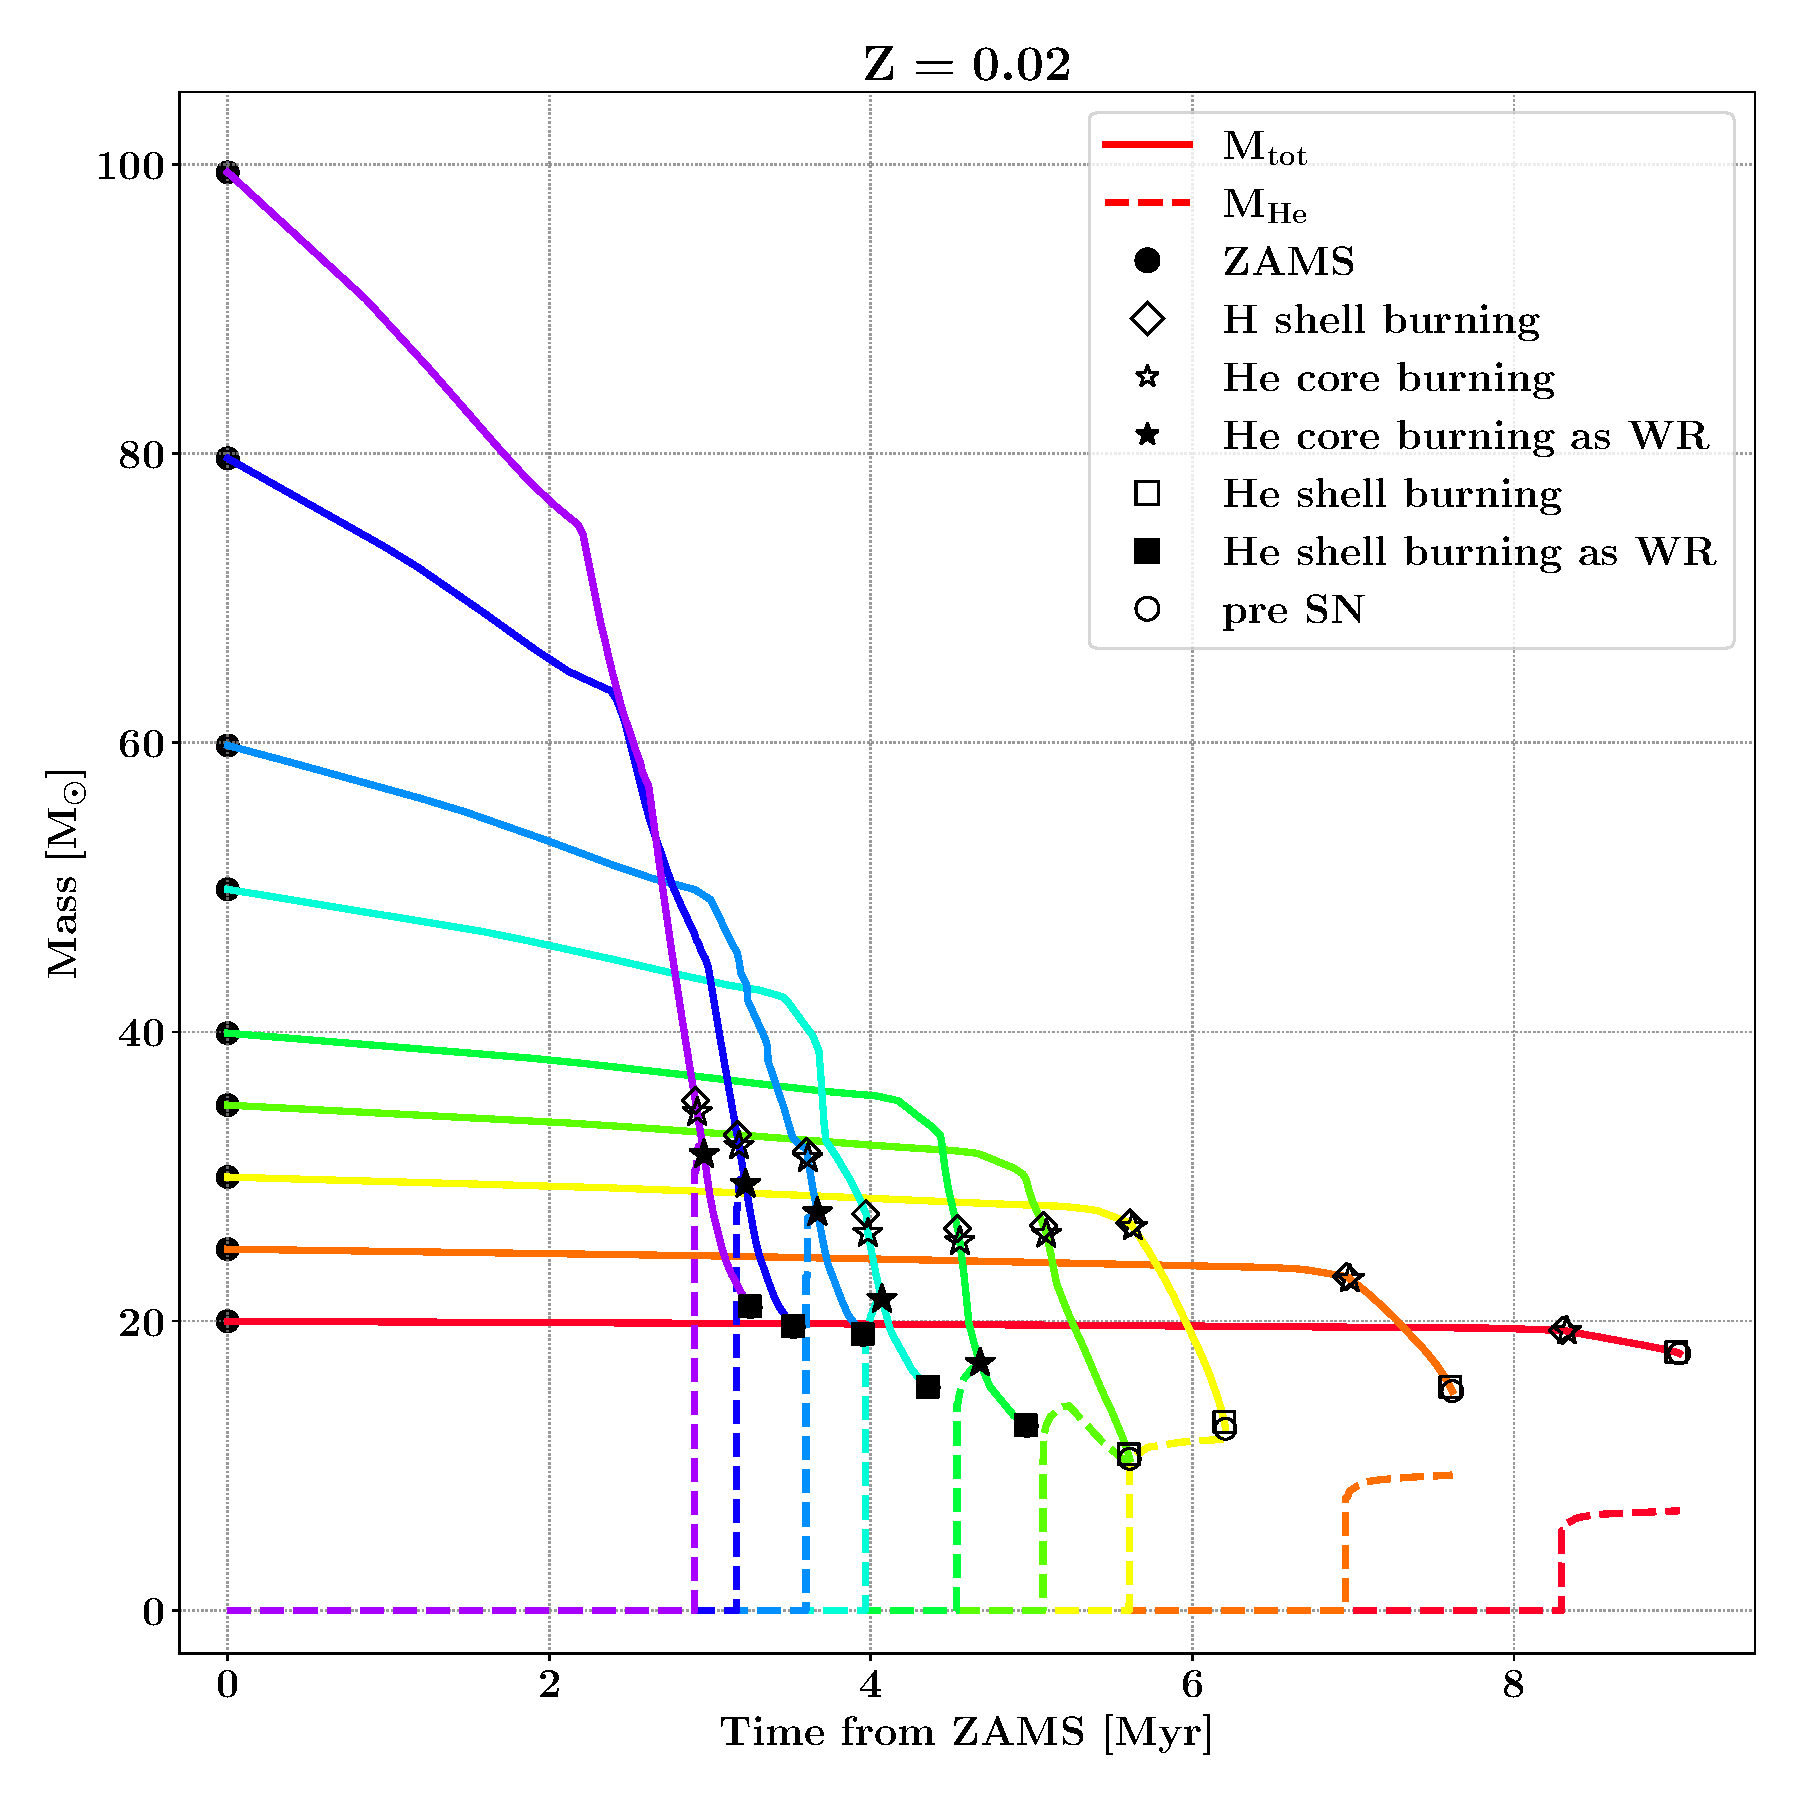
\includegraphics[width=1.05\textwidth]{./images/mass_Z02.pdf}
	\end{minipage}
	\hfill
	\begin{minipage}{.49\textwidth}
		\vspace{2mm}
		\centering
		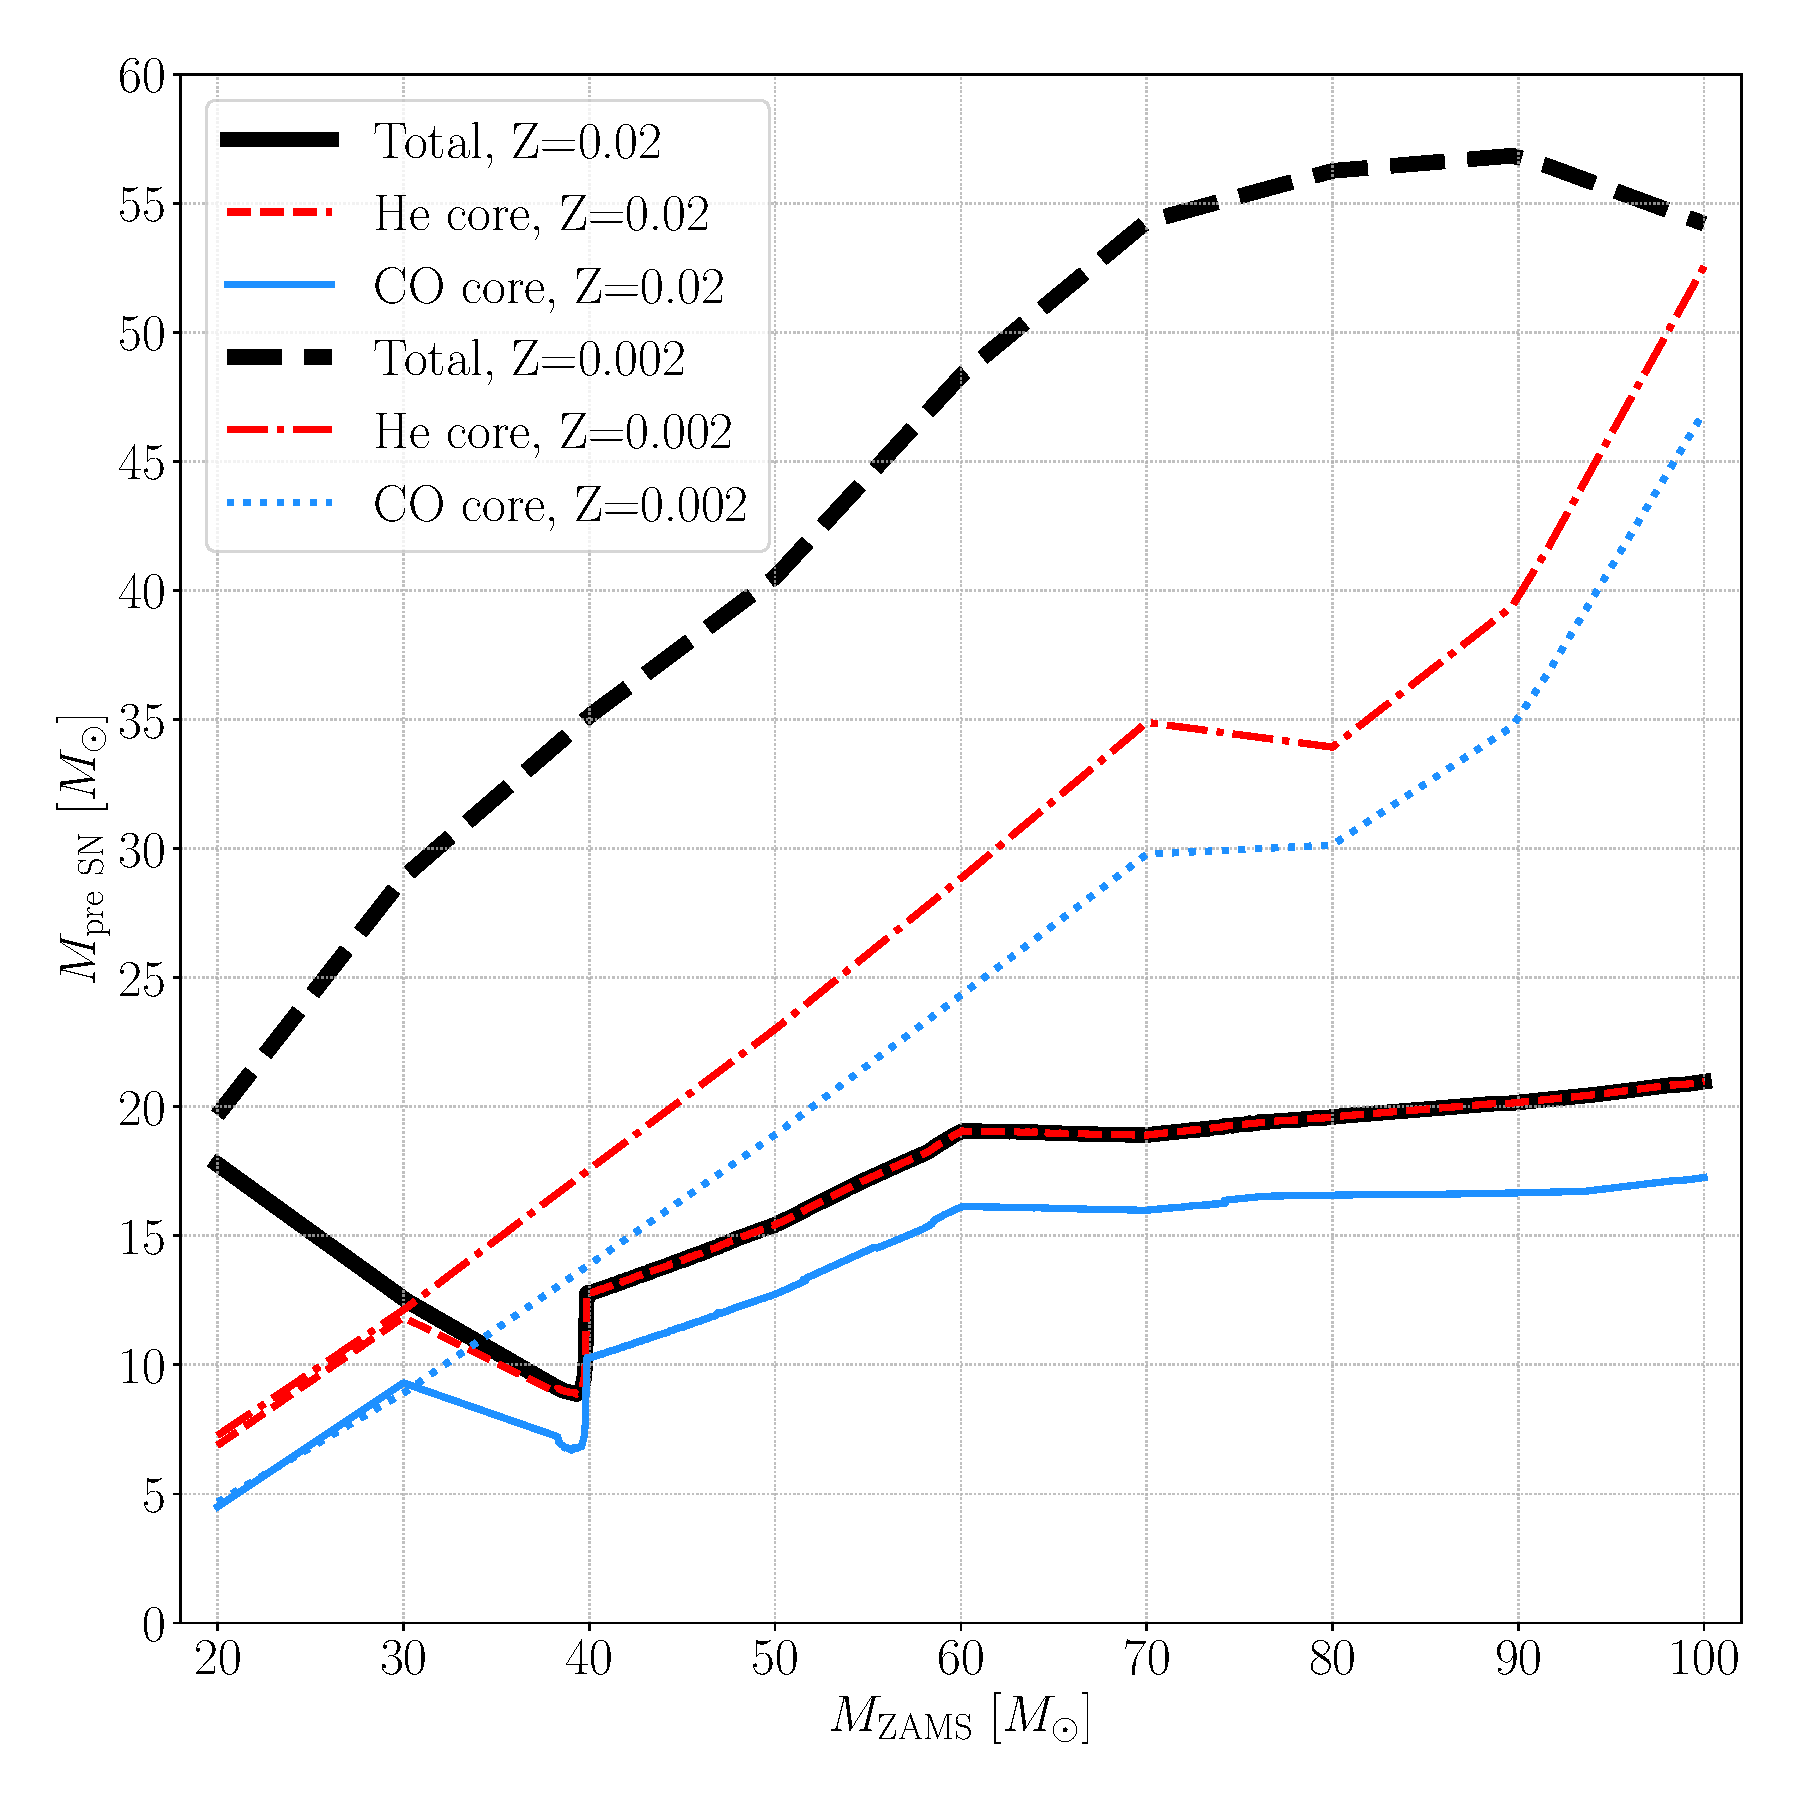
\includegraphics[width=1.05\textwidth]{./images/preSN.pdf}	
	\end{minipage}
	\caption{\emph{Left:} Time evolution of the mass of the stars (solid lines) and of their He cores (dashed lines) at solar metallicity. The symbols indicate the different burning stages, as explained in Sec.\ \ref{subsec:stellarevo}. \emph{Right:} Mass of the star and of their He and CO cores at the pre-SN stage, here coincident to the end of the CO burning. At solar metallicity the stellar winds strongly reduce the core sizes of stars with $\mzams \gtrsim 30 ~\msun$, transforming them into Wolf-Rayet for $\mzams \gtrsim 40 ~\msun$. At lower metallicity the cores and the stars are larger and they only reduce in stars with $\mzams \gtrsim 70-100 ~\msun$ that evolve too close to the Eddington limit. I generated both panels with the population-synthesis code \texttt{SEVN} \cite{spera2019_mergingBBH}, that interpolates the tables produced with the \texttt{PARSEC} stellar evolution code \cite{parsec2015_chen} (more details on the codes in Sec.\ \ref{sec:SEVN}).}\label{fig:masslostWR}
\end{figure}



\paragraph{Stellar evolution timescales} In this paragraph I briefly recall the main timescales that drive the single stellar evolution \cite{evostellare}. The time required for a star to react to a perturbation will determine not only its evolution but, if the star is a member of a binary system, will also influence the stability and efficiency of the mass transfer processes (further details in Sec. \ref{subsec:masstransfer}). \\

Stars are self-gravitating objects of hot plasma that remain in hydrostatic equilibrium throughout their life: the internal pressure gradient of the gas and photons is balanced by the self-gravity. According to the virial theorem, perturbations of the hydrostatic equilibrium occur on the \emph{dynamical timescale}

\begin{equation}\label{eq:taudyn}
\tau_\textup{dyn} \simeq \sqrt{\frac{R^3}{G M}} \simeq 30 \left(\frac{R}{R\sun}\right)^{3/2} \left(\frac{M\sun}{M}\right)^{1/2}\ \text{minutes}
\end{equation}


The energy released by the nuclear reactions is radiated from the surface and maintains the star in thermal equilibrium with $T_{\rm core} \approx const$. When the nuclear fuel is exhausted, the lower pressure gradient of the plasma causes a contraction of the star, in order to maintain the hydrostatic equilibrium. Part of the gravitational energy is radiated away but part of it heats up the interior, until it reaches the critical temperature to ignite heavier elements. The contraction is quasi-static and maintains the hydrostatic equilibrium. However, since a part of the energy produced by the contraction is not radiated away but heats up the interior, the process happens outside the thermal equilibrium and occurs in a \emph{thermal timescale} (also known as \emph{Kelvin-Helmholtz timescale})

\begin{equation}\label{eq:tauth}
\tau_\textup{th} \simeq \frac{G M^2}{R L} \simeq 15 
\left(\frac{M}{M\sun}\right)^{2} \left(\frac{R\sun}{R}\right) \left(\frac{L\sun}{L}\right)\ \text{Myr}
\end{equation}

Aside from central exhaustion or local fluctuations in the core temperature, a star evolves in thermal equilibrium. However, the longest evolutionary timescale is the \emph{nuclear timescale} and quantifies the time required to burn all the nuclear fuel for a given element. The longest nuclear timescale is the one for the hydrogen burning, that is the most abundant element ($\sim 70~\%$ of the stellar mass), and provides an order-of-magnitude estimate for the stellar lifetime

\begin{equation}\label{eq:taunuc}
\tau_\textup{nuc} \simeq 10 \left(\frac{M}{M\sun}\right) \left(\frac{L\sun}{L}\right)\ \text{Gyr}
\end{equation}

\paragraph{Stellar evolution from the ZAMS to the end of the CO burning} The star begin their life in the \emph{Zero Age Main Sequence} (ZAMS, filled circles) when their cores have temperatures $T_{\rm core} \gtrsim 10^{7}$ K elevated enough to ignite the hydrogen burning in the core. The evolution proceeds in the \emph{Main Sequence} (MS) phase until the central hydrogen is exhausted \cite{evostellare}. 

During the core H-burning phase, the stars satisfy the empirical mass-luminosity relation $L \propto M^3$. Recalling that the nuclear timescale $\tau_{\rm nuc}$ required to burn the hydrogen is an order-of-magnitude estimate of the stellar lifetime, the mass-luminosity relation of the Main Sequence substituted into the definition of the nuclear timescale of Eq.\ \ref{eq:taunuc} results in $\tau_{\rm nuc} \propto M^{-2}$: the more massive the star, the larger the luminosity caused by more efficient and rapid nuclear reactions, thus, the shorter the lifetime. For instance, the left-hand panel of Fig.\ \ref{fig:masslostWR} illustrates that, at solar metallicity, stars with $\mzams \sim 20~\msun$ live for $\sim 8$ Myrs, in contrast to more massive stars of $\mzams \sim 100~\msun$ that survive only for $\sim 3$ Myrs. Also, both stars have lifetimes much shorter than the Sun's $\sim 10$ Gyrs.

The stars considered here are so massive that they burn hydrogen in a large convective core surrounded by a radiative envelope. In the final stages of the core H-burning, the energy released diminishes and lowers the radiation pressure. To maintain the hydrostatic and thermal equilibrium, the core contracts and heats up again: the nuclear reactions increase again the luminosity produced and the surface effective temperature, thus, the star exhibits a left-ward hook in the Hertzsprung-Russel (HR) diagram (see Fig.\ \ref{fig:HRdiagrams}). \\

At the end of the core H-burning phase, the star is so contracted that the hydrogen shell surrounding the core is hot enough to ignite (empty diamonds). According to the mirror principle, if the layers below a burning shell contract then the layers above will expand. Stars with $\mzams \gtrsim 20~\msun$ have a core too massive to maintain the thermal equilibrium without a central burning, therefore, in the H-shell burning phase the star undergoes a core contraction and envelope expansion in a thermal timescale. Recalling Eq.\ \ref{eq:tauth} and Eq.\ \ref{eq:taunuc}, the thermal timescale is orders of magnitudes faster than the nuclear timescale: massive stars that burn hydrogen in their shells move so rapidly in the color-magnitude diagram during this phase that they are very unlikely to be observed, causing the so-called Hertzsprung-Gap (HG). \\


When the contraction heats up the core beyond $T_{\rm core} \gtrsim 10^{8}$ K, helium is ignited (empty stars). In theory, at this point the envelope has expanded and cooled so much that becomes convective and causes the star to evolve along the Hayashi line (an almost vertical line typical of stars dominated by the convective energy transport that with small variations in the super-adiabatic gradient can transport outward a wide range of luminosity for a given temperature). In reality, very massive stars will evolve close to the Eddington limit (black line in Fig.\ \ref{fig:HRdiagrams}) while the more metallic ones will suffer strong winds: in both cases, the net effects are depletion of the more external layers and exposition of the more internal and hot ones. Therefore, more massive and metallic stars will keep evolving in the blue region of the HR diagram and will eventually lose all the external hydrogen envelope, starting the core-He burning as Wolf-Rayet stars (filled stars). 

For instance, as shown in Fig. \ref{fig:HRdiagrams}, a $\mzams \sim 20~\msun$ star at solar metallicity $Z=0.02$ will start to burn helium in its core with an effective temperature of $T_{\rm eff} \sim 4~000$ K much cooler than the $T_{\rm eff} \sim 10~000$ K of the same star with metallicity $Z=0.002$ one order-of-magnitude smaller. Low-metallicity stars have quenched stellar winds that allow the star to retain and burn more mass: the core evolution is so fast that the external layers of the star are only slightly modified by the winds and survive beyond the Eddington limit (for instance, comparing the left- and right-hand panels of Fig.\ \ref{fig:HRdiagrams} it is evident that the markers of the burning stages are closer and in hotter positions for the less metallic stars). In contrast, stellar winds and instability near the Eddington limit strongly influence the evolution of stars with solar metallicity and $\mzams \gtrsim 35-40~\msun$ (left-hand panel of Fig.\ \ref{fig:HRdiagrams} and right-hand panel of Fig. \ref{fig:masslostWR}): the external layers are so much depleted that stars with $\mzams \gtrsim 40~\msun$ rapidly become Wolf-Rayet stars after a brief phase as LBV. The mass losses limit also the fuel to grow the He and CO cores: solar metallicity stars at the pre-supernova (pre-SN) stage have cores and total masses up to $\sim 30~\msun$ lighter with respect to the stars evolved at $Z=0.002$. While low-metallicity stars are mostly affected by the instability at the Eddington limit and the effect is relevant only for massive stars $\mzams \sim 70-100~\msun$, solar-metallicity stars are strongly depleted by their winds and the ones with $\mzams \gtrsim 40~\msun$ will explode as Wolf-Rayets of $M_{\rm WR} \sim 15-20~\msun$. In contrast, depletion is so irrelevant in single stellar evolution of low-metallicity stars that even stars up to $\sim 100~\msun$ do not form Wolf-Rayets at $Z=0.002$.\\

Stars that reach the core He-burning phase then evolve just in $\sim 10^{5}$ yrs towards a series of contractions and expansions where helium starts to burn in the shell (squares, filled if the stage is reached as a Wolf-Rayet or empty otherwise) and then CO starts to burn in the core, similarly to the evolution during the H-burning. \texttt{SEVN} stops the evolution of the star at the end of the CO-burning (empty circles) because the burning cycles of the heavier elements require detailed modelling of the star interior and occur in just few days. The supernova explosion and remnant properties are then calculated as a function of the mass of the CO core, as explained in Sec.\ \ref{subsec:SNmodels}.



\section{Mass transfer theory}\label{subsec:masstransfer}
\subsection{Conservative and non-conservative mass transfer}\label{subsec:conservativeMT}
The angular momentum $L$ of a binary system with circular orbit (for simplicity) of radius $a$ is

\begin{equation}\label{eq:L}
L = \mu\,a\,v_\textup{orb} = \frac{M_1 M_2}{M_1 + M_2} \sqrt{G \left(M_1 + M_2\right) a}
\end{equation}

where reduced mass $\mu$ and orbital velocity $v_{\rm orb}$ are functions of the stellar masses $M_1$ and $M_2$

\begin{equation}\label{eq:mu_vorb}
\mu = \frac{M_1 M_2}{M_1 + M_2} \quad \quad  v_\textup{orb}=\sqrt{\frac{G \left(M_1+M_2\right)}{a}} 
\end{equation}

\paragraph{Conservative case} If the orbital angular momentum $L$ and the total mass of the system $M_1 + M_2$ remain constant, the mass transfer is conservative. In this scenario, the relation of Eq.\ \ref{eq:L} becomes

\begin{equation}\label{eq:a_const}
a \left(M_1M_2\right)^2 = const
\end{equation}

and is showed in the left-hand panel of Fig.\ \ref{fig:masstransferRochelobe}. A system with primary $M_1 \geq M_2$ that transfers mass to the secondary $M_2$ shrinks its orbit until $M_2 \sim M_1$: when the accreting star becomes more massive than the donor, the orbit widens again.

\paragraph{Non-conservative case} Binaries can lose angular momentum and mass, for instance because of friction with the surrounding medium and because secondary stars are not able to accrete all the mass lost by the donors, respectively. Variations in the total angular momentum and mass of the system determine a non-conservative mass transfer and complicated models to determine the variation of the semi-major axis. From a qualitative point of view, Eq.\ \ref{eq:L} indicates a direct proportionality between orbital angular momentum and semi-major axis: the orbit shrinks if angular momentum is lost. Instead, Eq. \ref{eq:mu_vorb} suggests that less massive binaries have lower orbital velocities: energy conservation requires that the orbit widens \cite{Hurley2002}. 

Real binaries undergo non-conservative mass transfer episodes where the mass losses dominate over the orbital angular momentum losses. A binary mainly loses mass because of the combined effect of isotropic losses of the primary (especially through stellar winds or common envelope episodes, see Sec.\ \ref{subsec:windfed} and Sec.\ref{subsec:Commonenvelope}) and limited accretion of the secondary. 

\paragraph{Eddington limited accretion}
According to the virial theorem, a star in hydrostatic equilibrium that accretes mass converts part of its gravitational energy into radiation. In particular, the mass $M$ accreted over a timescale $\tau$ at rate $\mdot_{\rm acc} = M/\tau$ produces an accretion luminosity $L_{\rm acc}$ of

\begin{equation}
L_\textup{acc} = \frac{G M \mdot_{\rm acc}}{R}
\end{equation}

Imposing hydrostatic equilibrium requires that the accretion luminosity doesn't overcome the Eddington luminosity of Eq.\ \ref{eq:Eddingtonfactor}. The condition on the luminosity $L_{\rm acc} \leq L_{\rm Edd}$ becomes an upper limit to the maximum accretion rate allowed to maintain hydrostatic equilibrium

\begin{equation}\label{eq:Eddingtonaccretion}
\mdot_{\rm acc} \leq \dot{M}_\textup{Edd} = \frac{4 \pi c R}{k}
\end{equation}

The accretion rate is mainly limited by the star' size ($\dot{M}_\textup{Edd} \propto R$): only the larger stars can accrete rapidly a lot of mass. Eddington limited accretion strongly reduces mass accretion rates onto compact objects to almost negligible quantities ($\dot{M}_\textup{Edd} \sim\SI{e-8}{M\sun~\yr^{-1}}$ for a neutron star with radius $R\sim\SI{10}{\kilo\metre}$). Whether a compact object can or cannot accrete beyond the Eddington limit is still a matter of debate and is not the focus of this thesis, although theoretical modelling suggest that super-Eddington accreting compact objects should be unstable and could become exotic, like the \emph{Thorne-{\.Z}ytkow objects} \cite{binaries}.


\begin{figure}[h]
	\begin{minipage}{.55\textwidth}
		\centering
		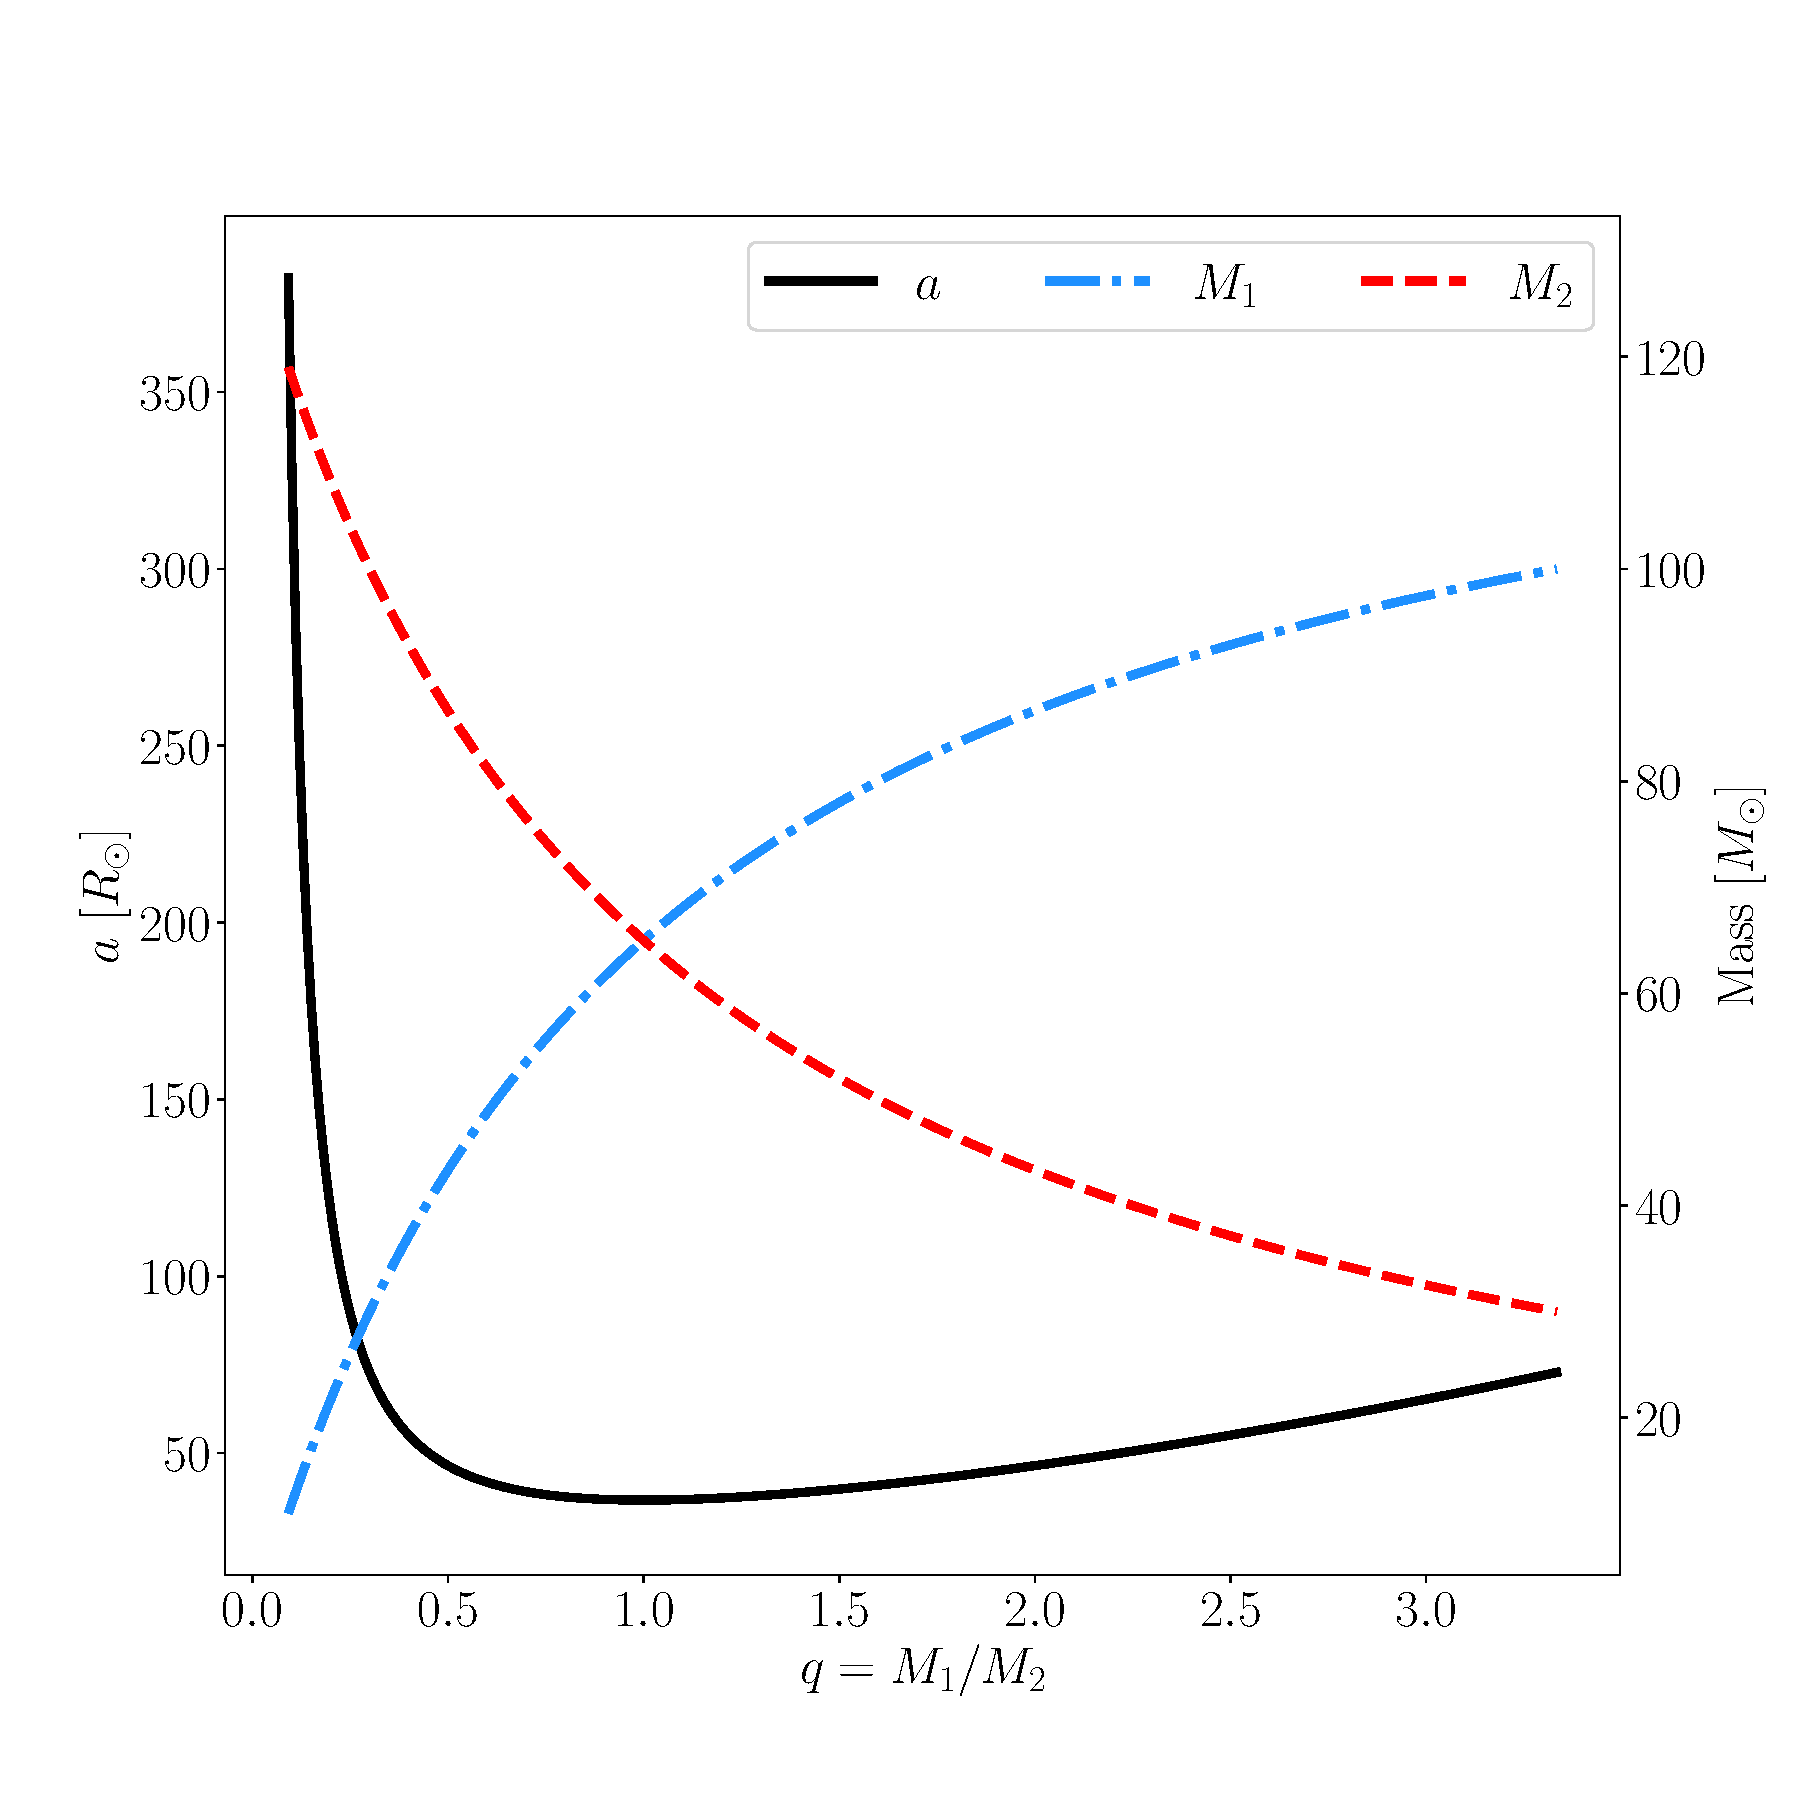
\includegraphics[width=\textwidth]{./images/masstransfer.pdf}
	\end{minipage}
	\hfill
	\begin{minipage}{.44\textwidth}
		\centering
		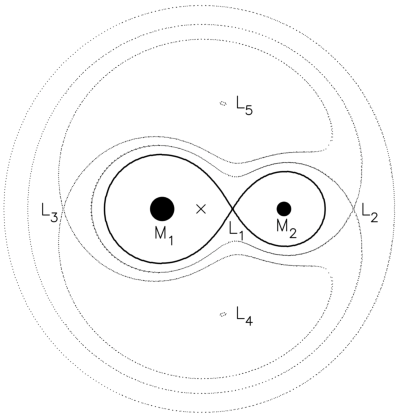
\includegraphics[width=\textwidth]{./images/Rochepotential.pdf}	
	\end{minipage}
	\caption{\emph{Left:} Conservative mass transfer from $M_1$ to $M_2$ first shrinks the semi-major axis of the orbit $a$ and then, when the secondary star becomes more massive than the primary $M_2 \geq M_1$, the orbit widens (see Eq.\ \ref{eq:a_const}). \emph{Right:} Orbital plane section of the equipotential curves of the Roche potential in the frame co-rotating with the binary. The Roche lobe is the black thick line containing the Lagrangian point $L_1$ \cite{tauris_evo_binaria}.}\label{fig:masstransferRochelobe}
\end{figure}

\subsection{Wind-fed binaries}\label{subsec:windfed}
Stellar winds cause an isotropic spread of the mass lost by the primary $M_1$, thus, it is reasonable to consider the secondary star $M_2$ as orbiting in a gas cloud. If the orbital velocity $v_{\rm orb}$ is small compared to the wind velocity $v_w \gg v_{\rm orb}$, accretion can be assumed spherical and described with the Bondi-Hoyle formalism \cite{BondiHoyle1944}: the average mass accreted over an orbital period by the secondary is

\begin{equation}\label{eq:accretionbondihoyle}
\langle \dot{M_2} \rangle = \frac{1}{\sqrt{1-e^2}} \left(\frac{G M_2}{v_w^2}\right)^2 \frac{\alpha_w}{2 a^2} \frac{1}{\left(1+v^2\right)^{3/2}} \dot{M_1}
\end{equation}

where $e$ is the eccentricity, $a$ the semi-major axis, $\alpha_w \approx 1.5$ an efficiency constant, $v$ is the ratio of the orbital velocity $v_{\rm orb}$ (calculated as in Eq.\ \ref{eq:mu_vorb}) and the wind velocity $v_w$ (calculated as the relative motion of the gas particles with respect to the secondary, proportional to the escape velocity with proportionality constant $\beta_w \approx 0.5-7$)

\begin{equation}
v = \frac{v_\textup{orb}}{v_w} \quad \quad v_w^2=2\beta_w \frac{G M_1}{R_1}
\end{equation}

Line-driven winds are one order-of magnitude faster than orbital velocities ($v_w \sim \SI{1000}{km/s}$ and $v_{\rm orb} \sim \SI{400}{km/s}$ \cite{CygX-3_Koljonen2017}): the $v$ term in Eq.\ \ref{eq:accretionbondihoyle} can be neglected and the average mass accreted becomes

\begin{equation}\label{eq:windfedaccretion}
\langle \dot{M_2} \rangle \propto \left(\frac{v_\textup{orb}}{v_w}\right)^4 \dot{M_1}
\end{equation}

The velocity ratio enters with the fourth power, strongly diminishing the efficiency of the wind-accretion: even enhanced mass losses of the primary $\mdot_1 \sim \SI{e-4}{\msun~\yr^{-1}}$ result in negligible accretion rates $\mdot_2 \sim \SI{e-8}{\msun~\yr^{-1}}$. Nevertheless, similar accretion rates are close to the ones allowed by Eddington-limited accretion onto compact objects (see Sec.\ \ref{subsec:conservativeMT}) and, even if small, are sufficient to power the formation and emission of the accretion disks in many X-ray binaries.

\subsection{Roche lobe overflow}\label{subsec:Rochelobeoverflow}
\paragraph{The Roche potential}
In the frame co-rotating with the binary, the sum of the gravitational and centrifugal potential is called Roche potential and its equipotential curves are shown in the right-hand panel of Fig.\ \ref{fig:masstransferRochelobe}. The potential wells of the stars become drop-shaped because of the orbital motion and are called Roche lobes. In order to describe them, in 1983 Eggleton \cite{Eggleton1983} introduced the Roche lobe radius $\rl$ as the radius of a sphere with volume equivalent to the one enclosed by a Roche lobe 

\begin{equation}\label{eq:rocheloberadius}
\rl = \frac{0.49~q^{2/3}}{0.6~q^{2/3} + \ln \left(1+q^{1/3}\right)}~a
\end{equation}

where $a$ is the semimajor-axis of the system and $q=M_1/M_2$ ($q=M_2/M_1$) is the ratio between the mass of the star belonging to the lobe $M_1$ ($M_2$) and its companion $M_2$ ($M_1$). The formula is obtained assuming circular and synchronized orbit, a condition often true for mass-transferring systems where the tight orbits are rapidly circularized and synchronized by tides.

\paragraph{Stability of the Roche lobe overflow} When a star expands beyond its Roche lobe (for instance because of stellar evolution or because the orbit shrinks), the layers outside the Roche lobe are no more bound to the star's potential well and can either be lost by the binary or accreted by the companion in the so-called Roche lobe overflow (RLO) process. The stability and efficiency of the RLO are still poorly understood and provide an active field of research because they depend on many factors, like the presence of a convective or radiative envelope and a core more or less prominent (both determine the response of the star to the removal of the external envelopes) or the possibility that the mass is transferred also from the external atmosphere of the star and outflows from the outer Lagrangian point of the donor (both determine the mass loss rates) \cite{marchant2021_masstransferMESA}.\\

A star that loses its external layers needs to re-adjusts its dimension in order to return in an equilibrium state. If the new equilibrium is achieved with a stellar radius still larger than the Roche lobe radius, the star will keep losing its outer layers in an unstable runaway that will lead the system to a common envelope (see Sec.\ \ref{subsec:Commonenvelope}). In contrary, if the star returns in the equilibrium state inside the Roche lobe, the RLO ends in a stable way. In this case, the stellar evolution may stimulate further expansions (for instance during the Hertzsprung-Gap phase or by igniting the core He-burning, as described in Sec.\ \ref{subsec:stellarevo}): the star can undergo a series of stable RLOs and transfer a large amount of mass. For instance, in 2002 Hurley et al.\ \cite{Hurley2002} proposed that stable RLO would lead to a mass loss rate strongly proportional to the amount of Roche lobe overfilling 

\begin{equation}\label{eq:masslostRoche}
    \mdot_1 \propto \left[ \ln \left(\frac{R_1}{\rlone} \right)\right]^3
\end{equation}

RLOs can be unstable over dynamical or thermal timescales, respectively for mass losses that perturb the hydrostatic or thermal equilibrium (see Sec.\ \ref{subsec:stellarevo}). As suggested by Webbink in 1984 \cite{Webbink1984_CE}, the (in)stability can be studied assuming that the radius is only a function of the mass $R\propto M^{\zeta}$ and, thus, comparing the logarithmic variation of the Roche lobe ($\zeta_L$) with the one induced in the stellar radius over the dynamical ($\zeta_\textup{ad}$)\footnote{The subscript ``ad'' recalls that dynamical perturbations act so rapidly that can be modelled as adiabatic processes.} or thermal ($\zeta_\textup{th}$) timescale

\begin{equation}\label{eq:zetaRLO}
\zeta_L = \frac{d \ln r_L}{d \ln M} \quad \zeta_\textup{ad} = \left(\frac{d \ln R}{d \ln M}\right)_\textup{ad} \quad \zeta_\textup{th} = \left(\frac{d \ln R}{d \ln M}\right)_\textup{th}
\end{equation}

The most rapid variation determines the dominant perturbation timescale, thus the reference mass-radius exponent $\zeta_* = \min\{\zeta_\textup{ad},\zeta_\textup{th}\}$ that, once compared to the Roche lobe variation $\zeta_L$, defines a Roche lobe overflow to be

\begin{equation}
\begin{cases}
\text{stable} &  \zeta_* \geq \zeta_L \\
\text{unstable} &  \zeta_* \leq \zeta_L
\end{cases}
\end{equation}

Inequality signs are a consequence of the negative denominators: the variation of the Roche lobe radius is referred to stars that are \emph{losing} mass ($d \ln M \leq 0$). As a reference, the left-hand panel of Fig.\ \ref{fig:RLOstability} shows a qualitative comparison between mass transfer episodes that are stable ($\zeta_* \geq \zeta_L$, S point), unstable on a thermal timescale but stable on the dynamical one ($\zeta_\textup{th} \leq \zeta_L \leq \zeta_\textup{ad}$, T point) or unstable on a dynamical timescale ($\zeta_\textup{ad} \leq \zeta_L$, P point).

\paragraph{Role of stellar envelopes, core sizes and mass ratios} The convective or radiative nature of the envelopes strongly affects the re-adjustments in the stellar structure after the removal of the external layers, eventually determining stability and efficiency of the RLOs. Radiative envelopes have a steep density gradient that prevents the onset of convection: the pressure exerted by the outer layers is so small that, once they are removed, the star almost does not need to expand to restore the equilibrium. Thus, stars with radiative envelopes have final radii usually lower than the initial ones ($\zeta_{\rm {ad}} \gg 0$) and will likely undergo stable RLOs. Convective envelopes, on the contrary, have an adiabatic structure that almost restores the initial radius via adiabatic expansion ($\zeta_{\rm {ad}} \lesssim 0$): similar stars will likely still overfill their Roche lobe after their re-adjustments and will enter unstable RLOs \cite{binaries} .\\

Stars that have a convective envelope and a central core or that are fully convective have been often modelled with, respectively, \emph{condensed} or \emph{complete} politropes\footnote{Convective envelopes, or full stars for the complete politrope case, were modelled with a politropic index $n=3/2$.} because of limited computational power. In 1987, Hjelliming \& Webbink used politropic models to study RLO instability on the dynamical timescale, finding that the core, when is present, increases the convective efficiency of the external envelope: stars lose more energy and reduce their radius as shown in the right-hand panel of Fig.\ \ref{fig:RLOstability}, likely avoiding an unstable RLO. The more evolved the star, the more the core becomes important in the structure: it grows in size and mass fraction because of the advanced nuclear burnings and of the removal of the external envelopes (caused by stellar winds and previous mass transfer episodes) \cite{hjellmingwebbink1987_coreRLOF} .\\

The binary mas ratio $q$ is another factor influencing the RLO stability, since it enters in the Roche lobe radius definition of Eq.\ \ref{eq:rocheloberadius}. As shown in the right-hand panel of Fig.\ \ref{fig:RLOstability}, if the donor star $M_1$ is much more massive than the companion $M_2$ ($q=M_1/M_2 \gg 1$) the more mass transferred and the more the potential well of the companion expands, shrinking the Roche lobe of the donor and facilitating the onset of an unstable RLO. On the contrary, stars with similar masses have similar Roche lobes with sizes modulated by the semi-major axis: assuming, as a reference, a conservative mass transfer as the one shown in the left-hand panel of Fig.\ \ref{fig:masstransferRochelobe}, systems with $q \sim 1$ have negligible changes in the semi-major axis extent, thus in the Roche lobe sizes. \\

\begin{figure}
	\begin{minipage}{.49\textwidth}
		\centering
		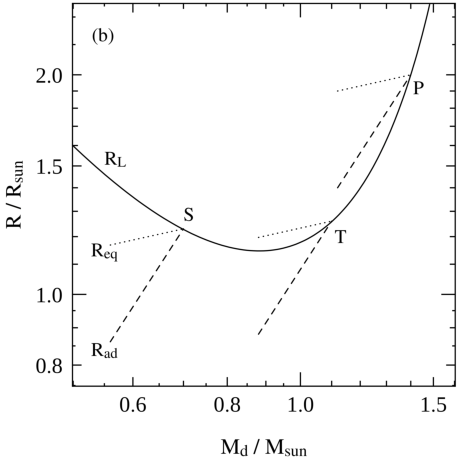
\includegraphics[width=\textwidth]{./images/stp_roche.pdf}
	\end{minipage}
	\hfill
	\begin{minipage}{.49\textwidth}
	    \vspace{-7mm}
		\centering
		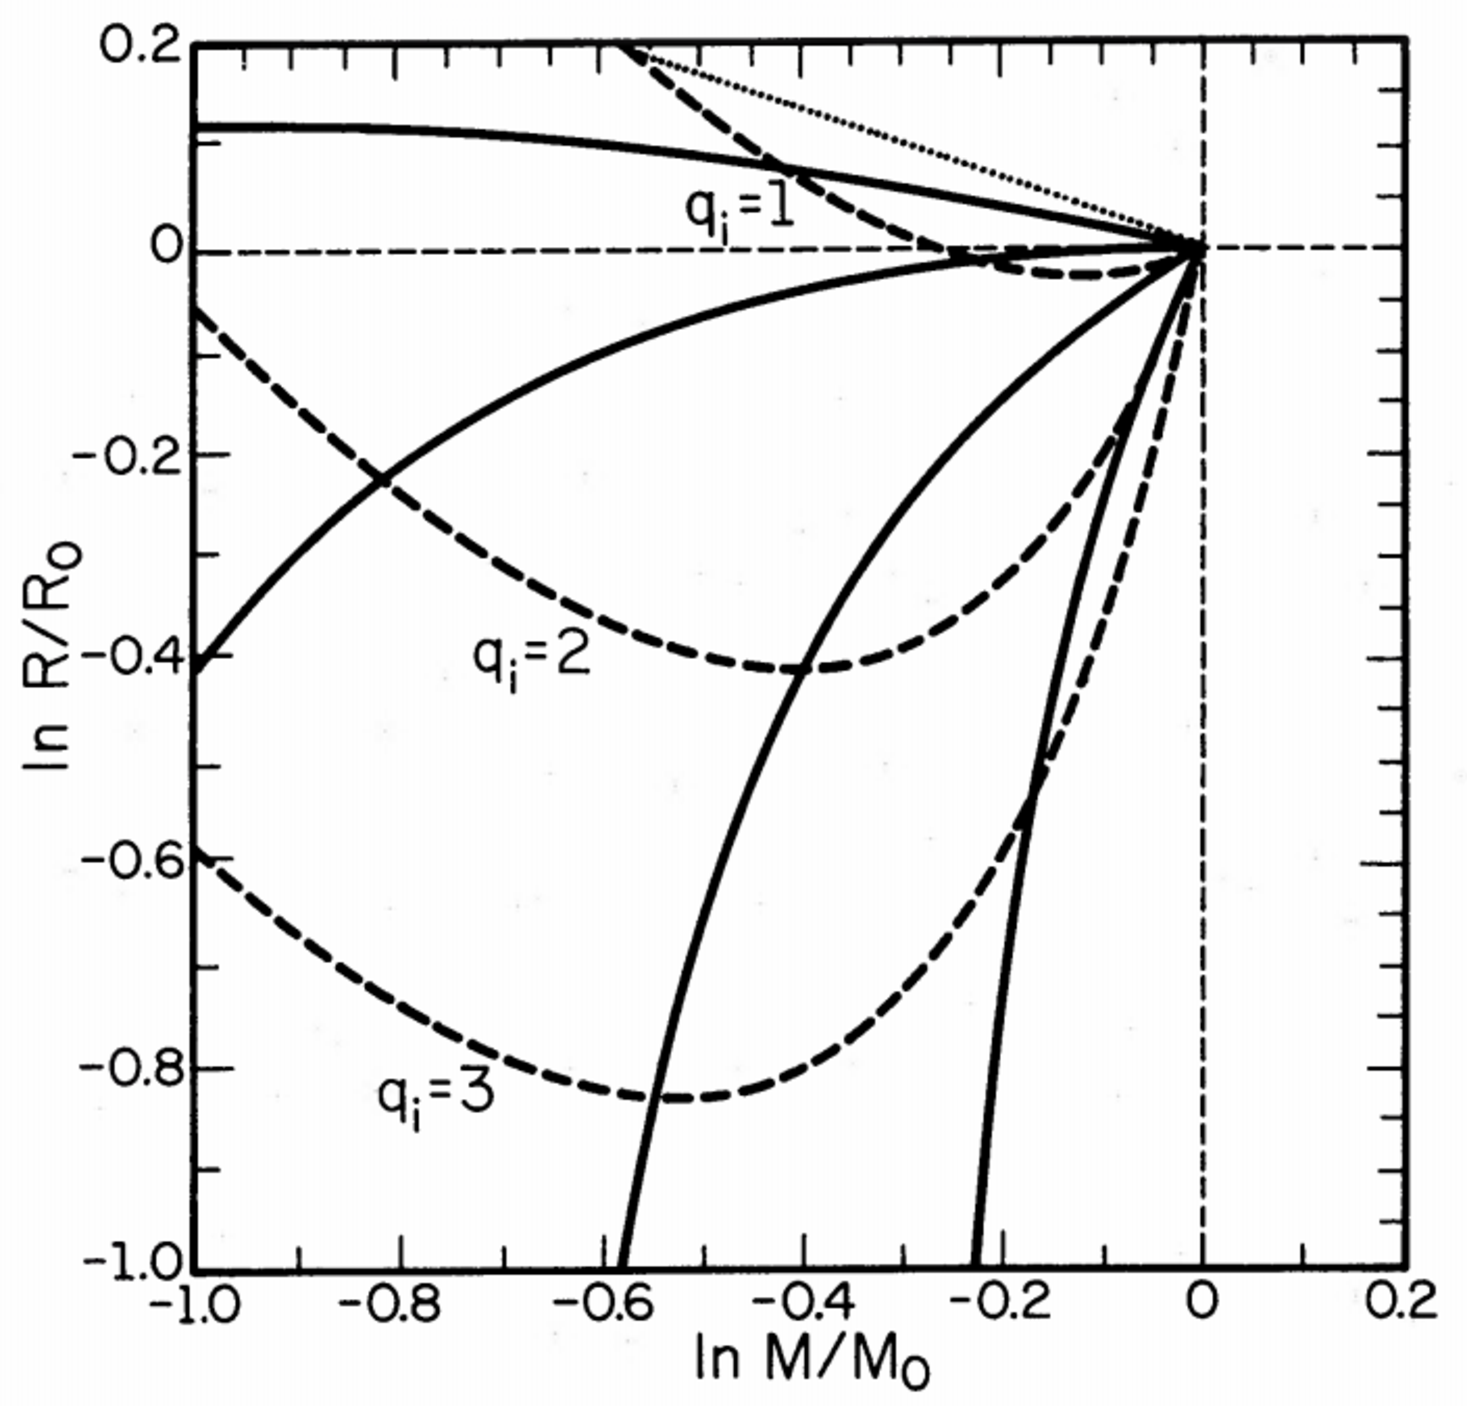
\includegraphics[width=\textwidth]{./images/core_he_rlof.pdf}	
	\end{minipage}
	\caption{\emph{Left:} Examples of the RLO (in)stability scenarios for a $\SI{2}{\msun}$ binary with fixed donor mass-radius exponents ($\zeta_\textup{ad}=1.5$ and $\zeta_\textup{th}=\zeta_\textup{eq}=0.25$, illustrated respectively by the dashed and dotted lines). Different donor masses determine different Roche lobe radii (solid line, Eq.\ \ref{eq:rocheloberadius}), thus the same adjustment to the mass loss ($\zeta_*$) might determine a RLO stable ($\zeta_* \geq \zeta_L$, S point), stable on the dynamical timescale but unstable on the thermal one ($\zeta_\textup{th} \leq \zeta_L \leq \zeta_\textup{ad}$, T point) or unstable also on the dynamical timescale ($\zeta_\textup{ad} \leq \zeta_L$, point P) \cite{binaries}. \emph{Right:} Adiabatic variation of the stellar radius as a function of the mass lost ($R_0$ and $M_0$ are the values before the mass loss). Solid lines: condensed politropes with growing core sizes (from top to bottom $q_\textup{core}$=0.10, 0.25, 0.50, 0.75). Dotted line: complete politrope, models a fully convective star with $n=3/2$. Dashed lines: Roche lobe radii for different initial mass ratios (from top to bottom $q_i=M_{\rm don}/M_{\rm acc}=1,2,3$). A convective star may avoid a dynamically unstable RLO if it has a prominent core $q_{\rm core} \gg$ or it has a companion with similar mass $q \sim 1$ \cite{hjellmingwebbink1987_coreRLOF}.}\label{fig:RLOstability}
\end{figure}


Many works in the literature started from the above considerations to obtain models and thresholds that could numerically determine whether or not a binary system would enter a stable or unstable mass transfer. Similar models often are too much simplified and calibrated on old stellar tracks (or even to politropes) but provide a fast and easy-to-implement method to calculate the RLO (in)stability in population-synthesis codes. For instance, many codes (including the one adopted in this thesis, \texttt{SEVN} \cite{spera2019_mergingBBH}) derived part of their mass transfer prescriptions from the formalism suggested in 2002 by Hurley et al.\ for the \texttt{BSE} code \cite{Hurley2002}. These codes assume a one-to-one correspondence between the burning stage, the radiative/convective nature of the envelope and the core size, starting a RLO unstable on the dynamical timescale when the mass ratio $q=M_{\rm donor}/M_{\rm accretor}$ is larger than a given threshold $q_{\rm crit}$, calibrated with stellar evolution models and function of the core size $q_{\rm core}=M_{\rm core, donor}/M_{\rm donor}$

\begin{equation}\label{eq:qcrit}
	q \geq q_\textup{crit} \left(q_\textup{core}\right)
\end{equation}

Unfortunately, recent studies pointed out that there is not an unique correlation between the burning stage, the extent of the radiative/convective envelope, the core size and the RLO (in)stability \cite{klencki2020_mtproblems}. Moreover, many of the values for the $q_{\rm crit}$ and mass loss rates (like the one of Eq.\ \ref{eq:masslostRoche}) were obtained from old stellar tracks (or politropic models) that did not properly model the more massive stars, suggesting that an updated and corrected modelling of the mass transfer that accounts for up-to-date stellar evolution is required.



\subsection{Common envelope}\label{subsec:Commonenvelope}
\paragraph{A key-process in binary evolution} Stars that enter an unstable RLO (see Sec.\ \ref{subsec:Rochelobeoverflow}), collide\footnote{Collision occur for two stars larger than the orbital separation at periastron $R_1 + R_2 > (1-e)~a$.} or are part of a contact binary\footnote{Contact binaries form when both stars overfill their Roche lobes $R_1 \geq \rlone$ and $R_2 \geq \rltwo$.} share a part or all of their envelopes (if present), thus, orbit in a medium denser than the interstellar one. Binaries evolving in similar \emph{common envelope} (CE) configurations lose orbital angular momentum and energy because of friction with the surrounding gas: the orbit shrinks while the gas heats up and eventually disperses.  Depending on the initial orbital energy, envelope potential energy and efficiency in the energy and angular momentum transfer, binaries can either spiral-in and merge or be able to eject the common envelope: in the latter case, only the nuclei survive and the orbit tightens.

Common envelope processes shrink efficiently the orbits and are determinant to form tight compact object binaries that can merge via emission of gravitational waves within a Hubble time \cite{spera2019_mergingBBH}. However, only systems with the right combination of stellar and orbital properties can survive to common envelopes events. For instance, the orbit must be wide enough not to merge too rapidly and both stars should have a well-developed core: the latter condition prevents the core mass to be transferred into the common envelope and allows the star to survive as a self-gravitating object. A summary of the main formation channels and outcomes of the CE evolution is shown in Fig.\ \ref{fig:ce_mapelli}.

It is important to point out that evolution through a CE phase efficiently removes the hydrogen envelope to one or both stars. Therefore, common envelope is a key-process to form Wolf-Rayet stars and its role will be further discussed in the results of this thesis, presented in Sec.\ \ref{sec:results}.


\begin{figure}
	\centering
	\def\svgwidth{0.9\textwidth}
	\import{./images/}{ce_schema.pdf_tex} 
	\caption{Possible initial and final common envelope configurations. The two stars are represented with cores (blue for the primary, black for the secondary) and envelopes (orange) but it could also be that one of the two star has not yet developed a core (e.\ g.\ a Main Sequence star), is already envelope-stripped (e.\ g.\ a Wolf-Rayet star) or is a compact object (e.\ g.\ a black hole). A binary may enter a CE after an unstable RLO, a collision or after being a contact binary. The H-rich envelope of one or both stars are shared and if at least one of the stars is missing a core, the two are merged. In contrast, the two nuclei (or a nucleus/Wolf-Rayet and a compact object) could survive the spiral-in if the initial orbit is wide enough to eject the envelope, heating the gas through friction. The scheme is inspired by figure no. 7 of Mapelli, 2019 \cite{mapelli} and based on the mass transfer implementation in \texttt{SEVN}, described in Sec.\ \ref{subsec:masstransferSEVN}.}\label{fig:ce_mapelli}
\end{figure}


\paragraph{$\boldsymbol{\alpha \lambda}$ formalism} The most widely adopted description for common envelope processes is the bi-parametric one proposed by Webbink in 1984 \cite{Webbink1984_CE}. They assume that orbital energy is the only energy source to power the envelope removal and they model the energetic balance with two adimensional parameters: $\alpha$ and $\lambda$.

The $\alpha$ parameter indicates the fraction of orbital energy  $E_{\rm orb}$ used to eject the common envelope

\begin{equation}\label{eq:EorbCEalpha}
\Delta E_\textup{orb} = \alpha \left(E_\textup{orb, f} - E_\textup{orb, i}\right) = \alpha \frac{G M_\textup{c,1} M_\textup{c,2}}{2} \left(\frac{1}{a_\textup{i}} - \frac{1}{a_\textup{f}}\right)
\end{equation}

where $M_\textup{c,1}$ and $M_\textup{c,2}$ are the two core masses and $a_\textup{i}$ and $a_\textup{f}$ are the initial and final semi-major axis, respectively . Because of friction, the orbit shrinks, thus $a_\textup{f} < a_\textup{i}$ and $\Delta E_\textup{orb} \leq 0$.

The $\lambda$ parameter is related to the common envelope concentration: small values of $\lambda$ indicate concentrated envelopes, more difficult to eject. In particular, $\lambda$ is related to the envelope binding energy of the single stars through dimensional considerations

\begin{equation}\label{eq:EenvCElambda}
E_\textup{env} = - \frac{G}{\lambda} \left(\frac{m_\textup{env,1} M_1}{R_1}+ \frac{m_\textup{env,2} M_2}{R_2}\right)
\end{equation}

where $R$, $M$ e $m_\textup{env}$ are respectively radius, mass and envelope mass of each star at the onset of common envelope.

Imposing that the orbital energy lost by the system equals the common envelope binding energy ($\Delta E_\textup{orb} = E_\textup{env}$), it is possible to obtain the system final semi-major axis as function of the $\alpha$ and $\lambda$ parameters

\begin{equation}\label{eqn:a_ce}
\frac{1}{a_\textup{f}} = \frac{1}{\alpha \lambda} \frac{2}{M_\textup{c,1} M_\textup{c,2}} \left(\frac{m_\textup{env,1} M_1}{R_1}+ \frac{m_\textup{env,2} M_2}{R_2}\right) + \frac{1}{a_\textup{i}}
\end{equation}

The direct proportionality relation $a_\textup{f} \propto \alpha\lambda$ indicates that binaries with more chances of survival ($a_{\rm f} >$) are the ones that have poorly concentrated envelopes ($\lambda >$) and efficiently converted the orbital energy into heat ($\alpha >$). \\

Even though the $\alpha \lambda$ formalism is easy-to-implement and widely adopted in population-synthesis codes, there is general consensus in the literature that it needs to be updated with a more detailed and self-consistent treatment of stellar and binary evolution \cite{marchant2021_masstransferMESA}. Many observed systems suggest that likely $\alpha > 1$, meaning that additional forms of energy need to be considered to eject the common envelope \cite{mapelli}. Moreover, current implementations adopt $\lambda$ values obtained from fits to various stellar evolution models even though  a self-consistent calculation should be preferred. In particular, fits to single stellar evolution tracks do not account for changes in the binding energy due to mass transfer events and their result are sensitive to the internal energy sources considered. For instance, in 2021 Marchant et al.\ \cite{marchant2021_masstransferMESA} pointed out that 2014 fits from Claeys et al.\ \cite{Clayes2014_lambdaCE}, widely implemented in population-synthesis codes (including the one adopted in this thesis, \texttt{SEVN}, see Sec.\ \ref{subsec:masstransferSEVN}), underestimate the binding energy of stars that frequently enter a CE, like Hertzsprung-Gap stars, overestimating the number of systems that survive the CE and, eventually, merge as binary black holes. In 2021 Gallegos-Garcia et al.\ \cite{gallegos2021MESAvspopsynth} further demonstrated that, at least for H-rich donor stars, current prescriptions for entering an unstable RLO and surviving the common envelope may overestimate by a factor $\sim 5-500$ the binary black hole merger rates, favouring too much the formation through CE evolution in systems that, instead, likely evolve through stable RLOs as shown in Fig.\ \ref{fig:MESAvsPopsynth}.

\begin{figure}[h!]
		\centering
		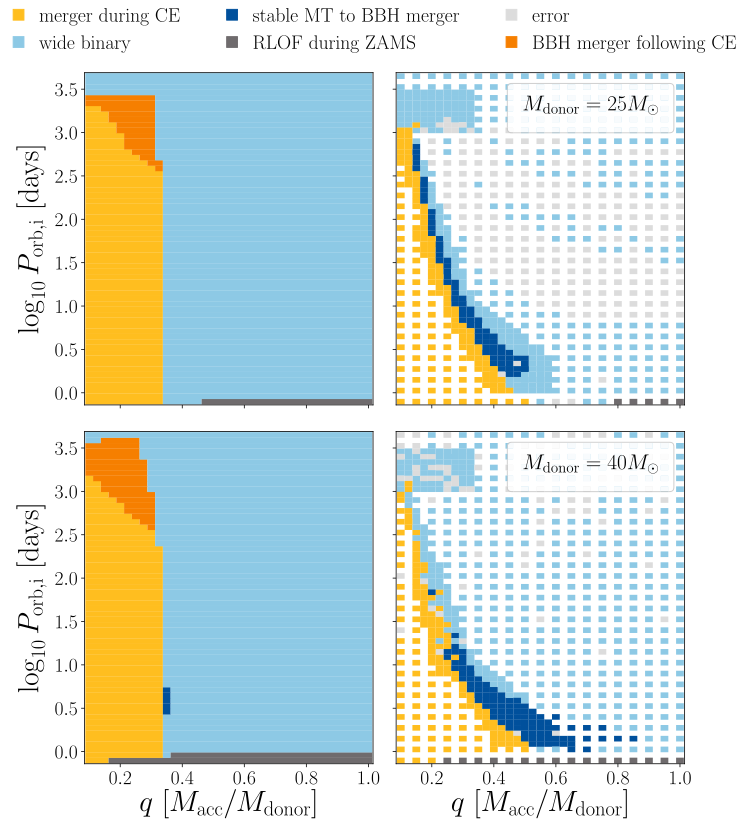
\includegraphics[width=0.9\textwidth]{./images/MESAvspopsynth.png}	
	\caption{Comparison of final outcomes for the same initial binary population evolved with the \texttt{COSMIC} population-synthesis code \cite{breivik2020cosmicpopsynth} (\emph{left}) and with the \texttt{MESA} stellar evolution code, which also implements modules for binary evolution \cite{MESA2015BinaryMT} (\emph{right}). Each row shows the initial period as a function of the initial mass ratio for H-rich donors of $M = 25~\msun$ (top) and $M = 40~\msun$ (bottom) at sub-solar metallicity $Z=0.00142$. On-the-fly stellar and binary evolution carried out in \texttt{MESA} suggests that only a restricted parameter space region successfully forms binary black holes (BBHs), in contrast with results from population-synthesis codes. \texttt{MESA} BBHs formed mainly through stable RLO, whereas CE evolution dominated for \texttt{COSMIC} BBHs \cite{gallegos2021MESAvspopsynth}.}\label{fig:MESAvsPopsynth}
\end{figure}


%%%%%%%%%%%%%%%%%%%%%%%%%%%%%%%%%%%%%%%
%%%%% END OF "DEFINITIVE" PART %%%%%%%%
%%%%%%%%%%%%%%%%%%%%%%%%%%%%%%%%%%%%%%%

% paperino

%%%%%%%%%%%%%%%%%%%%%%%%%%%%%%%%%%%%%%%%%%%%%%%%%%%%%%%%%%%%%%%%%
%%%%%%%%%% WORK IN PROGRESS BELOW %%%%%%%%%%%%%%%%%%%%%%%%%%%%%%%
%%%%%%%%%%%%%%%%%%%%%%%%%%%%%%%%%%%%%%%%%%%%%%%%%%%%%%%%%%%%%%%%%



\section{Observed candidates of Wolf-Rayet -- black hole systems}\label{sec:WRBHobserved}

\subsection{Overview of WR--BH properties and fates}
Only seven systems are candidated as Wolf-Rayet -- black hole binaries (hereafter, WR--BH): their main parameters and uncertainties are listed in Tab.\ \ref{tab:observations} \cite{observations}. General properties of WR--BH systems are presented in this section while in the next ones I will discuss the characterization of each system.


\paragraph{Masses and periods} As explained in Sec.\ \ref{subsec:Xraymeasure} and Sec.\ \ref{subsec:massWR}, X-ray light curves and UV, optical, near-IR spectra are the main tools used to characterize stellar and binary properties. While they provide precise estimates of the orbital period, the masses are often so poorly constrained that it is not possible to determine whether some compact objects are neutron stars or black holes, although further X-ray observations suggest a mild preference for a black hole in Cyg X-3 and IC10 X-1. 

Spectroscopic observations ensured the Wolf-Rayet nature of the companion in Cyg X-3, IC10 X-1, NGC300 X-1 and M101 ULX-1. In contrast, CXOU J123030.3+413853, CXOU J004732.0-251722.1 and CG X-1 are more uncertain as WR--BH binaries and their classification is based only X-ray measurements, since spectral observations were not available.  Moreover, the uncertain candidates are hosted in starburst galaxies, further supporting the possibility of being at least High-Mass X-ray binaries (see Sec.\ \ref{subsec:cygx3observations}, \ref{subsec:IC10X1_revisedmasses}, \ref{subsec:uncertainWRcandidates} for a detailed discussion on the single system properties).


\paragraph{Fates} Even though the masses estimates are quite uncertain, all the Wolf-Rayets are massive enough to collapse into a black hole: the WR--BH systems are likely progenitors of binary black holes (see Sec.\ \ref{subsec:stellarevo}). Using the formula derived in 1964 by Peters \cite{Peters1964}, it is possible to obtain an order-of-magnitude estimate for the time needed to merge via GW emission $t_\textup{GW}$:

\begin{equation}\label{eq:tgw}
t_\textup{GW} = \frac{5}{256} \frac{c^5 a^4 (1-e^2)^{7/2}}{G^3 M_1 M_2 (M_1 + M_2)}
\end{equation}

where $G$ is the gravitational constant, $c$ is the speed of light and $a$ is the semi-major axis. For simplicity, it is reasonable to assume that the orbital period of the binary black hole will be similar to the one observed in the WR--BH configuration (simulated systems discussed in Sec.\ \ref{sec:results} show that the WR--BH period is indeed little affected by the supernova kick and remains almost identical when a binary black hole forms). Following \cite{observations}, the reference compact object binary is assumed to have circular orbit (eccentricity $e=0$), secondary BH of $M_{2,\rm BH} \sim 10~\msun$ produced by the WR and primary BH of $M_{1,\rm BH} \sim 10~\msun$. Such masses are probably smaller than the real ones but allow to obtain an upper boundary for $t_\textup{GW}$. Under these assumptions, WR--BH systems need to have a period $P \lesssim 10~$ days ($a \lesssim 20~\rsun$) in order to merge within a Hubble time. By comparing this value with the ones reported in the Table \ref{tab:observations}, all binary systems formed with characteristics similar to the observed WR-BH candidates could produce a merging binary black hole observable today, with the exception of systems like M101 ULX X-1 that are too wide to merge within a Hubble time.


%%%%%%%%%%%%%%%%%%%%%%%%%%
%%%%%%%%%%%%%%%%%%%%%%%%%
\begin{figure}[h]
    \centering
	\begin{threeparttable}
		\begin{tabular}{llcccccc}
			\toprule
			\multirow{2}{*}{Host galaxy} & \multirow{2}{*}{Name} & $M_{\rm BH}$ & $M_{\rm WR}$ & $P$ & $t_\textup{GW}$  &  Z & $d$ \\
			& & [$\msun$] & [$\msun$] & [hours] & [Gyr] & [$\zsun$] & [Mpc]\\
			\midrule
			Milky Way & Cyg X-3 & 3 & 7 &4.8 & 0.017 & 0.92 & 0.00741 \\
			IC 10 & IC10 X-1 & 23-33\tnote{a} & 35\tnote{b} & 34.9\tnote{a} & 3.5  & 0.22 & 0.70\\
			NGC 300 & NGC300 X-1 & 13-21\tnote{d} & 26\tnote{c} & 32.8\tnote{d} & 2.9  & 0.19 & 2.02\\
			NGC 253 & CXOU J004732.0-251722.1 & - & - & 14.5 & 0.33  & 0.24 & 3.0 \\
			Circinus & CG X-1 & - & - & 7.2 & 0.051  & 0.10 & 4.2 \\
			M101 & M101 ULX-1 & 20-30 & 19& 196.8 & 348 & 0.17 & 6.9\\
			NGC 4490 & CXOU J123030.3+413853 & - & - & 6.4 & 0.038  & 0.23 & 8.55\\
			\bottomrule 	
		\end{tabular}
		\begin{tablenotes}[para]
			\item[a]\cite{IC10X-1_Silverman2008} 
			\item[b]\cite{IC10X-1_Clark2004_WRmass}
			\item[c]\cite{NGC300X-1_Crowther2010} 
			\item[d]\cite{NGC300X-1_Binder2021_BHpreciso}
		\end{tablenotes}
		\centering
		\captionof{table}{Properties of the seven WR-BH candidates. Table inspired by \cite{observations}. Masses and periods are extracted from papers referenced with the superscripts. $t_\textup{GW}$ is an order-of-magnitude estimate for the time to merge via gravitational-wave emission and is calculated with Eq.\ \ref{eq:tgw} assuming the same observed period and $M_{1,\rm BH} = M_{2,\rm BH} = 10~\msun$, given the uncertainties in the mass determination discussed in Sec.\ \ref{sec:WRBHobserved}. Distances and metallicities refer to the host galaxies as in \cite{observationsZSFR_Mapelli2010a} for all binaries except for Cyg X-3: its distance is taken from \cite{CygX-3_McCollough2016_Observation} and is used to infer the local metallicity from the Milky Way metallicity gradient \cite{MetallicityGradientMW2018Gaia}, as explained in Sec.\ \ref{subsec:cygx3observations}.} \label{tab:observations}
	\end{threeparttable}
\end{figure}
%%%%%%%%%%%%%%%%%%%%%%%%%
%%%%%%%%%%%%%%%%%%%%%%%%%




\subsection{Cyg X-3}\label{subsec:cygx3observations}
%Review of Koljonen+2017 and discussion on why values of Zdiarski+2013 are not reliable and we don't use them. Also describe it is in the MW and how we determined its metallicity and distance.

Cyg X-3 is the only known WR--BH candidate in the Milky Way: being at almost solar metallicity, it will become a case-study binary in this thesis work and its possible evolutionary pathways will be discussed in Sec.\ \ref{sec:results}. Hereafter I will present the key observations that characterized Cyg X-3, underlying the ones that will be used as fiducial model in this thesis.



%\paragraph{Observations and identifications}
%Cyg X-3 lies in the galactic plane therefore no optical/UV counterpart has been detected yet due to interstellar absorption (\cite{CygX-3_Koljonen2017}). Thus we know that the companion is a WR only by observing its IR spectrum. Using IR and X-ray emission lines, the companion is a low-mass BH or a NS.

\paragraph{Distance}
X-ray and sub-millimetric observations revealed that Cyg X-3 has a nearby Bok globule located 15.6" away from the binary, as shown in the left-hand panel of Fig.\ \ref{fig:CygX3}. This Cyg X-3 ``little friend '', as it is sometimes called, is a cloud of gas and dust of $\sim 2-24~\msun$ with $\sim 0.2$ pc diameter and is associated with a star-forming region. Observations of the 1.3 mm CO line revealed a velocity shift of $\SI{-47.5}{km/s}$. Since the cloud belongs to the Galactic plane, it is reasonable to assume that the Doppler shift is dominated by the rotational velocity. However, the Bok globule is close to the Perseus arm and there have been evidences of anomalous motion of objects in that region. Thus, in 2016 McCollough et al.\ \cite{CygX-3_McCollough2016_Observation} used a Bayesian tool that could account for errors in the estimated kinematic distances, finding that the Bok globule has 62 \% of probability of being at $d_{\rm Bok} = 6.08 \pm 0.64$ kpc and 38 \% probability of being at $d_{\rm Bok} = 7.85 \pm 0.6$ kpc.

X-ray light curves of this Bok globule exhibit the same period modulation of Cyg X-3 but are shifted in phase by $\Delta \phi = 0.56$, suggesting that X-ray photons emitted by the binary are scattered by the dust cloud towards the observer. The small angular separation between the Bok globule and Cyg X-3 coupled with the observed time delays allow to use geometrical arguments to determine the distance of Cyg X-3. Using the previously determined relative distance of the Bok globule of $d_{\rm Bok} = 6.08 \pm 0.64~ (7.85 \pm 0.6)$ kpc , McCollough et al.\ found that Cyg X-3 is distant $0.82 \pm 0.09~ (0.77 \pm 0.07)$ kpc from the Bok globule and $d_{\rm Cyg~X-3} = 7.41 \pm 1.13~ (10.16 \pm 1.21)$ kpc from the observer. The first estimate relies on the most probable value for the Bok globule's distance, therefore can be used as reference value for the Cyg X-3 distance

\begin{equation}\label{eq:distanceCygX3}
    \boxed{d_{\rm Cyg~X-3} = 7.41 \pm 1.13 ~\rm kpc}
\end{equation}



Assuming that the supernova explosion forming the compact object of Cyg X-3 occurred $\sim 1-5$ Myrs ago (average lifetime of a Wolf-Rayet, see Sec.\ \ref{subsec:stellarevo}) and that Cyg X-3 originally formed in that Bok globule, the relative distance of $\sim 1$ kpc suggests a natal kick of 190-980 km/s. Both distances and natal kick estimates are consistent with independent calculations in the literature, although the work of McCollough et al.\ provides the most precise distance determination.

\paragraph{Metallicity}
In 2018 Lemasle et al.\ \cite{MetallicityGradientMW2018Gaia} used distances and metallicities of twenty-five Cepheids from the Gaia Data Release 2 to estimate the Milky-Way metallicity gradient, finding the relation

\begin{equation}\label{eq:MWmetallicitygradient}
    [\rm Fe/H]=-0.0447~d_{\rm Gal} + 0.3522
\end{equation}

where $d_{\rm Gal}$ is the Galactocentric distance expressed in kpc units.

Assuming, as Lemasle et al.\ \cite{MetallicityGradientMW2018Gaia}, that the Sun has a Galactocentric distance of $d_{\rm \odot,Gal} = 7.94$ kpc and recalling, as McCollough et al.\ \cite{CygX-3_McCollough2016_Observation}, that Cyg X-3 lies on the Galactic plane ($l=79.84^\circ, b=+0.70^\circ$) with relative distance to the Sun of $d_{\rm Cyg~X-3} = 7.41 \pm 1.13$ kpc, I used trigonometric relations to infer the Galactocentric distance of Cyg X-3 as $d_{\rm Cyg~X-3, Gal} = 9.85$ kpc. At this distance, the metallicity of the Milky-Way estimated through the gradient of Eq.\ \ref{eq:MWmetallicitygradient} as [Fe/H] = -0.088. 

Assuming that the metallicity distribution of the Sun is universal \cite{metallicityFeHconversion}, the [Fe/H] metallicity of any star can be converted into metal mass fraction $Z$ with the relation 

\begin{equation}
    [\rm Fe/H]_* = \log(Z/X)_* - \log(Z/X)_\odot
\end{equation}


where $X$ is the hydrogen mass fraction. For a star at the Galactocentric distance of Cyg X-3, the metal content is thus

\begin{equation}\label{eq:CygX3metallicity}
    \boxed{Z_{\rm Cyg~X-3} = 0.916~\zsun}
\end{equation}

This metallicity is the one reported in Tab. \ref{tab:observations} for Cyg X-3 and is clearly very similar to the solar one, given that both the Sun and Cyg X-3 have almost the same Galactocentric distance. In particular, assuming standard solar metallicity of $\zsun =0.02$ implies $Z_{\rm Cyg~X-3} = 0.018$ while using 2011 updated determinations from Caffau et al.\ \cite{caffau2011solarmetallicity} $\zsun=0.015$ indicate $Z_{\rm Cyg~X-3}=0.014$.


\paragraph{Period} Cyg X-3 light curves and spectra exhibit a strong modulation of 4.8 hours ($\sim 4^{\rm h} 48^{\rm m}$). In particular, in 2002 Singh et al.\ \cite{CygX-3_Singh2002} obtained very accurate values for period $P$ and period derivative $\dot{P}$ from parabolic fits to X-ray light curves

\begin{equation}\label{eq:periodCygX3}
    \boxed{P_{\rm Cyg~X-3} = 4^{\rm h} 47^{\rm m} 32.735^{\rm s}~\pm~0^{\rm h} 0^{\rm m} 0.008^{\rm s}}
\end{equation}

\begin{equation}\label{eq:pdotCygX3}
    \boxed{\dot{P}/P_{\rm Cyg~X-3} = (1.05 \pm 0.04) \times 10^{-6}~\yr^{-1}}
\end{equation}

As pointed out by Zdziarski et al. in 2013 \cite{Cyg-X3_Zd2013}, the period of Cyg X-3 is unusually short for an High-Mass X-ray binary and suggests a past spiral-in episode, likely due to a common envelope (see Sec.\ \ref{subsec:Commonenvelope}). This interpretation is supported also by the results of this thesis, as discussed in Sec.\ \ref{sec:results}.

\paragraph{Masses} So far only IR spectra are available for Cyg X-3: since the binary lies on the Galactic plane, strong interstellar absorption prevented the observation of optical an UV counterparts \cite{CygX-3_Koljonen2017}. The spectra revealed the presence of strong He I and He II lines, classifying the Wolf-Rayet as a WNL sub-type (see Tab.\ \ref{tab:WRclassification}).\\

As explained in Sec.\ \ref{subsec:Xraymeasure} and Sec.\ \ref{subsec:massWR}, it is possible to use a mass-luminosity relation to determine the mass of a Wolf-Rayet and then couple this information with period and maximum amplitude of the radial velocity curve to obtain the dynamical mass of the companion compact object. In 2013, Zdiarski et al.\ \cite{Cyg-X3_Zd2013} used IR spectra extracted in 1999 by Hanson et al.\ \cite{CygX-3_Hanson2000wrongspectrum} and mass-luminosity relations for WN stars calibrated in 2000 by Nugis \& Lamers \cite{Nugis2000_WRwinds} to estimate a Wolf-Rayet mass of $\mwr = 10.3_{-2.8}^{+3.9}~\msun$ and a compact object mass of $M_C = 2.4_{-1.1}^{+2.1}$. However, in 2017 Koljonen \& Maccarone \cite{CygX-3_Koljonen2017} pointed out that the spectra of Hanson et al.\ \cite{CygX-3_Hanson2000wrongspectrum} were taken in an outburst state, where the variability of 2.058 $\mu m$ He I absorption line (used to extract the radial velocity curve) was not tracing the orbital motion of the Wolf-Rayet but, instead, reflected the ionization structure of the wind. Similar misinterpretations occurred also for NGC 300 X-1 and IC 10 X-1 and caused a revision of their masses, as explained in more detail in the next section (Sec.\ \ref{subsec:IC10X1_revisedmasses}). \\

In 2017, Koljonen \& Maccarone \ \cite{CygX-3_Koljonen2017} extracted new IR spectra of Cyg X-3 and re-estimated its compact object mass. Assuming a distance of $d_{\rm Cyg~X-3} = 7.41 \pm 1.13~ (10.16 \pm 1.21)$ kpc from McCollough et al.\ \cite{CygX-3_McCollough2016_Observation}, they estimated the absolute K-band magnitude to be $M_K = -4.2 \pm 0.4~(-4.9 \pm 0.3)$ mag and used the \texttt{PoWR} non-LTE atmosphere models for WN stars \cite{WRnonLTEatmospheresPoWR_Todt2015} to derive a corresponding luminosity of $L_{WR} = 5.32 \pm 0.16~(5.59 \pm 0.12)~\lsun$. In 2011, Gr{\"a}fener et al.\ \cite{Grafener2011_M-L_WR} extracted the mass-luminosity relations for non-homogeneous core-He burning stars showed in the left-hand panel of Fig.\ \ref{fig:MLandwinds} from stellar models also based on \texttt{PoWR}. Thus, Koljonen \& Maccarone self-consistently used the Gr{\"a}fener et al.\  mass-luminosity relations and determined the Wolf-Rayet masses to be $\mwr = 8-10~(11-14)~\msun$. The corresponding mass losses of $\mdot = (0.4-1.3) \times 10^{-5}~((0.6-2.0)\times 10^{-5})~\msun~\yr^{-1}$ are extracted from the \texttt{PoWR} models and are then corrected for wind clumping. Overall, the Wolf-Rayet mass is consistent with the one found in 2013 by Zdiarski et al.\ \cite{Cyg-X3_Zd2013} and, accounting for the possible errors in the distance estimates of McCollough et al.\ \cite{CygX-3_McCollough2016_Observation}, can be conservatively assumed to be

\begin{equation}\label{eq:MWRCygxX-3}
    \boxed{M_{\rm WR,~Cyg~X-3} = 8-14~\msun}
\end{equation}

As previously pointed out and further discussed in the next section, the strong helium lines in the IR spectrum are not reliable tracers of the orbital motion but rather reflect variability in the Wolf-Rayet winds. Therefore Koljonen \& Maccarone adopted a different strategy to determine the mass of the Cyg X-3 compact object. They assumed that all the isotropic wind flowing past the accretion radius of the compact object $r_{\rm acc}$ is accreted

\begin{equation}\label{eq:massaccretedBHCygX3}
    \mdot_{\rm acc} \approx \frac{\pi r_{\rm acc}^2}{4 \pi a^2} ~ \mdot
\end{equation}

where the semi-major axis $a$ is determined from Kepler's third law and the accretion radius $r_{\rm acc}$ is a function of the relative wind velocity at the location of the compact object $v_{\rm rel}$

\begin{equation}
    a = \sqrt[3]{\frac{P^2 G (\mwr + M_C)}{4 \pi}} \qquad \qquad r_{\rm acc} \sim \frac{2 G M_C}{v_{\rm rel}^2} 
\end{equation}

Back-substituting $a$ and $r_{\rm acc}$ into Eq.\ \ref{eq:massaccretedBHCygX3} results in

\begin{equation}\label{eq:massaccreted2}
    \mdot_{\rm acc} \approx 0.0176 \times \left( \frac{1000~\rm km/s}{v_{\rm rel}} \right)^4 \left( \frac{4.8~\text{hrs}}{P} \right)^{4/3} \frac{M_C^2}{(\mwr + M_C)^{2/3}}   ~ \mdot
\end{equation}

Assuming that only the wind confined within the orbit falls to the compact object $r_{\rm acc} < a$ implies, according to Eq.\ \ref{eq:massaccretedBHCygX3}, that only <1/4 of all the mass lost by the Wolf-Rayet $\mdot$ is accreted. A similar and reasonable assumption, coupled with the well-know period of $P=4.8$ hrs \cite{CygX-3_Singh2002} and the previously estimated Wolf-Rayet mass loss rates of $\mdot = (0.4-2.0)\times 10^{-5}~\msun~\yr^{-1}$ \cite{CygX-3_Koljonen2017} reduce Eq.\ \ref{eq:massaccreted2} into a simple relation between the two masses and the relative wind velocity $v_{\rm rel}$, showed in the right-hand panel of Fig.\ \ref{fig:CygX3}. 

$v_{\rm rel}$ is determined by the wind terminal velocity $v_{\inf}$ and orbital velocity $v_{\rm  orb}$ through $v_{\rm rel}^2 = v_{\inf}^2 + v_{\rm orb}^2$. \texttt{PoWR} atmosphere models predict a terminal wind velocity of $v_{\inf} \approx 700-800$ km/s. In contrast, the orbital velocity is less precise $v_{\rm orb} \approx 300-750$ km/s due to the large uncertainty in the orbital inclination $i \approx 30^{\circ}-70^{\circ}$. Overall, the wind relative velocity at the compact object location is not higher than $v_{\rm rel} \lesssim 750-1000$ km/s, implying a compact object with mass $M_C \lesssim 5-10~\msun$ (see the right-hand panel of Fig.\ \ref{fig:CygX3}). 

\paragraph{Black hole or neutron star?}
The maximum allowed mass for a neutron star lies is $M_{\rm NS,max}\sim 2.5-3~\msun$, according to theoretical studies on the equation of state and on observations of double neutron stars and pulsars \cite{NSreview}. Therefore, in principle, the compact object in Cyg X-3 could be either a black hole or a neutron star. However, in 2013 Zdiarski et al.\ \cite{Cyg-X3_Zd2013} pointed out that the X-ray and radio spectra in the hard and soft state of Cyg X-3 resembled the ones of X-ray binaries that are known to contain a black hole. Even though they found a dynamical mass range in between a neutron star and a black hole $M_C = 2.4_{-1.1}^{+2.1}$ (adopting the unreliable He I absorption lines, though), they argued that the aformentioned circumstantial evidences were sufficient to support the black hole nature of the compact object. 

Further evidence for the black hole hypothesis comes from the 2022 study of Antokhin et al.\ \cite{CygX-3_Antokhin2022}. They obtained a more precise estimate of the inclination $i = 29.5^{\circ} \pm 1.2^{\circ}$ that further supports the $M_C \lesssim 10~\msun$ upper limit. Moreover, assuming a smooth Wolf-Rayet wind, they propose a compact object mass of $M_C \approx 7.2~\msun $ even they though recognize that, due to the many uncertainties in the wind modelling, the neutron star hypothesis cannot be completely ruled out.

In this thesis, I will follow the black hole hypothesis and, since \texttt{SEVN} sets the maximum neutron star mass to be  $M_{\rm NS,max} = 3~\msun$ \cite{spera2019_mergingBBH}, the mass of the compact object in Cyg X-3 will be hereafter considered to lie in the range

\begin{equation}\label{eq:MBHCygX3}
    \boxed{M_{\rm BH,~Cyg~X-3} = 3-10~\msun}
\end{equation}

\paragraph{Wind-fed system} Given the well-known period of $P=4.8$ hours and considering a Wolf-Rayet of $\mwr = 8-14~\msun$ with a black hole companion of $\mbh = 3-10~\msun$, the total mass of Cyg X-3 is $M_{\rm tot} = 11 - 24~\msun$ and, according to Kepler's third law, results in a semi-major axis of $a \sim 3-4~\rsun$. From Eq.\ \ref{eq:rocheloberadius}, the Roche Lobe radius would be of $\sim 2-2.5~\rsun$, small enough to be exceeded by the Wolf-Rayet radius (Wolf-Rayet stars typical have Sun-like radii). However, Koljonen \& Maccarone \cite{CygX-3_Koljonen2017} recalled that population-synthesis results obtained in 2005 by Lommen et al.\ \cite{CygX-3_Lommen2005_Ppdot} indicated that systems like Cyg X-3 have a negligible probability to be observed in the Roche lobe overflow configuration and, even if the system would have an active RLO, it would last $\ll 100~$ yrs. Therefore, Cyg X-3 is reasonably considered a wind-fed system, a configuration that will be consistent also with the results of this thesis, presented in Sec.\ \ref{sec:results}. 



\begin{figure}
	\begin{minipage}{.49\textwidth}
		\centering
		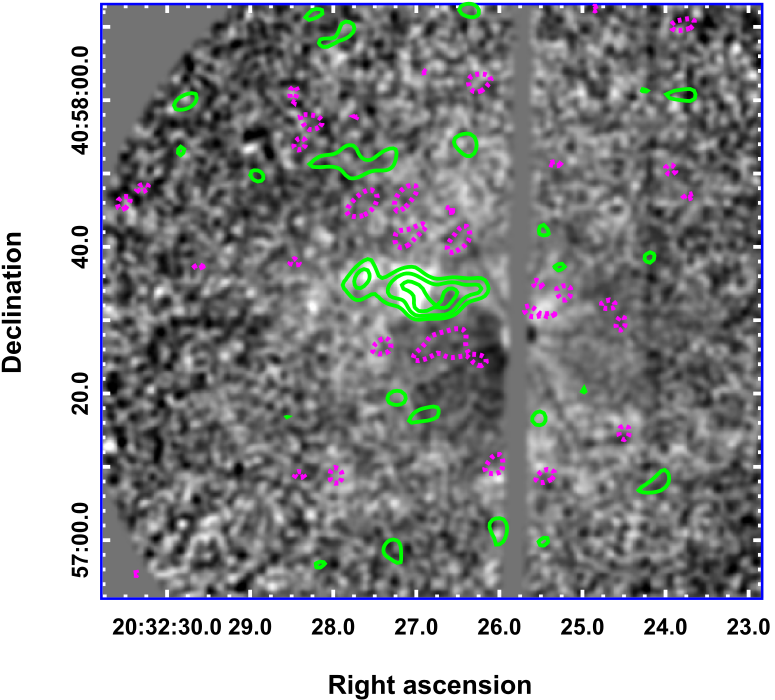
\includegraphics[width=\textwidth]{./images/CygX3littlefriend.png}
	\end{minipage}
	\hfill
	\begin{minipage}{.49\textwidth}
		\centering
		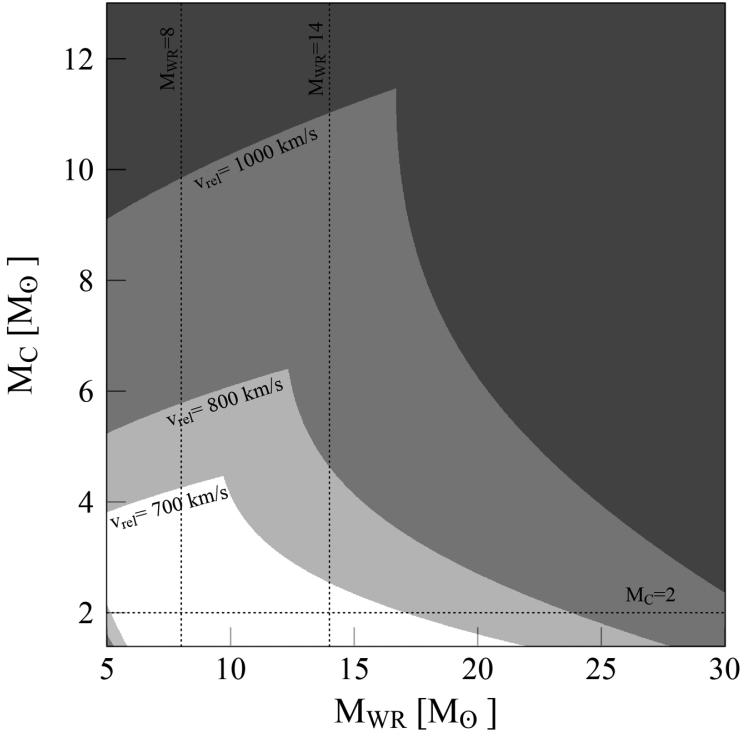
\includegraphics[width=\textwidth]{./images/CygX3massBH}	
	\end{minipage}
	\caption{\emph{Left:} Gray-scaled X-ray image of Cyg X-3 and its ``little friend''. The PSF of Cyg X-3, centered at $(\alpha \approx 26^{\rm h}, \delta \approx 30^{\circ})$, was subtracted. Sub-millimetric contours of the CO line at $-47.5$ km/s are overlaid, in green if positive and magenta if negative. The Bok globule is identified by the denser green contours superimposed to the bright X-ray blob on the left of Cyg X-3 \cite{CygX-3_McCollough2016_Observation}. \emph{Right:} Possible compact object masses $M_C$ as a function of Wolf-Rayet masses $\mwr$ with descreasing values of relative wind velocities at the location of the compact object $v_{\rm rel}$. The most probable values of $\mwr = 8-14~\msun$ and $v_{\rm rel} \lesssim 750-1000$ km/s favour a compact object with mass $M_C \lesssim 5-10~\msun$, most likely a black hole \cite{CygX-3_Koljonen2017}.}\label{fig:CygX3}
\end{figure}


\subsection{IC10 X-1, NGC300 X-1, M101 ULX-1}\label{subsec:IC10X1_revisedmasses}


\paragraph{Dynamical mass revisions}
Discutere dei venti e del ritardo di fase in laycock 2015 e binder 2021



\begin{figure}[h]
	\begin{minipage}{.39\textwidth}
		\centering
		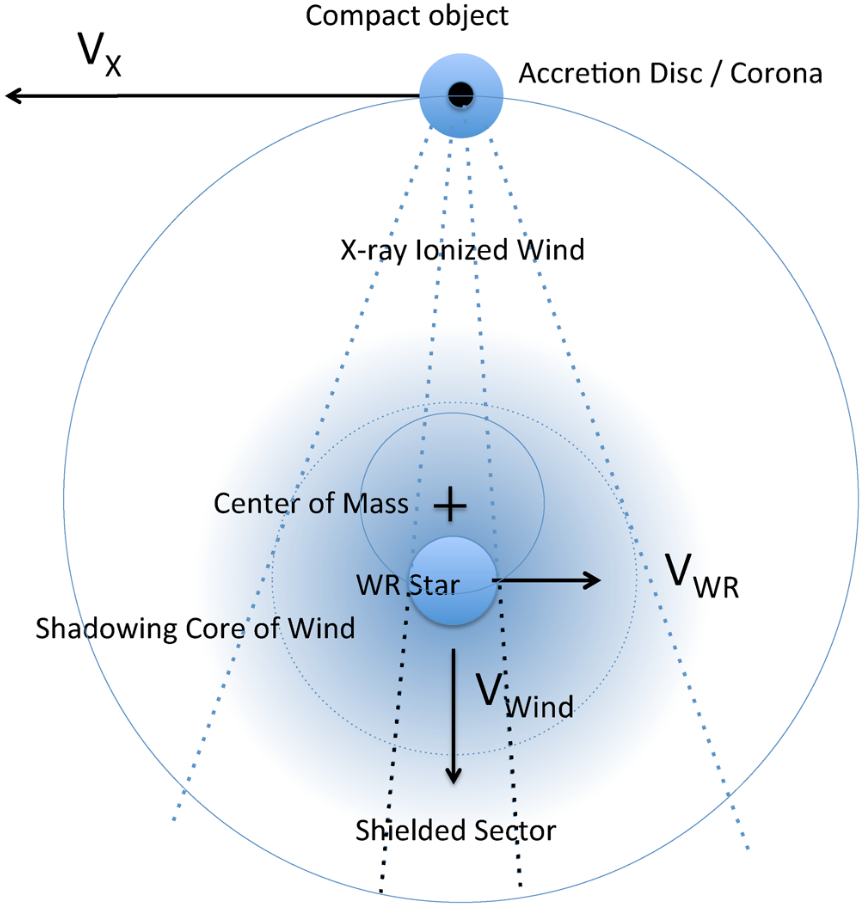
\includegraphics[width=\textwidth]{./images/WRwindIC10X-1.png}
	\end{minipage}
	\hfill
	\begin{minipage}{.60\textwidth}
		\centering
		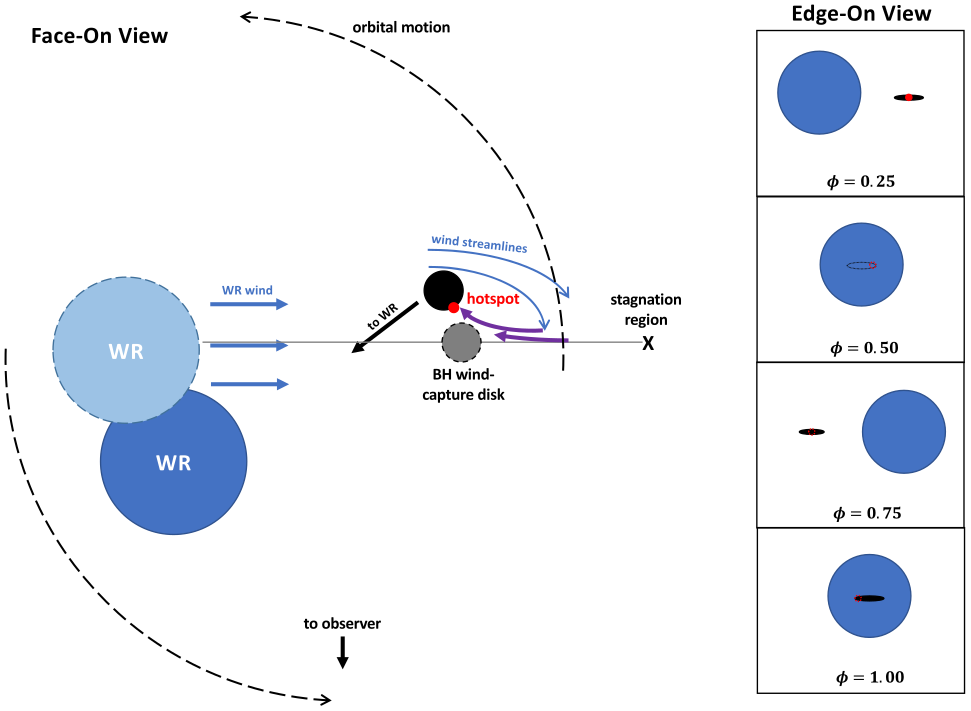
\includegraphics[width=\textwidth]{./images/WRwindNGC300.png}	
	\end{minipage}
	\caption{yjdtymx,y}\label{fig:WRBHwind}
\end{figure}
ADD UPDATED MEASURES FOR IC 10 X-1 AND CHECK THE OTHERS


\subsection{CXOU J123030.3+413853, CXOU J004732.0-251722.1, CG X-1}\label{subsec:uncertainWRcandidates}

In particular, the WR--BH classification is based interpreting the slow rises and fast decays of the X-ray light curve with regions of stronger and lighter interaction between the ionized matter of the Wolf-Rayet winds and the X-radiation, in analogy with the light curve modulations of Cyg X-3, that is known to host a WR and a compact object.





% hereafter the text from Computation astrophysics

On one hand, spectroscopic observations confirmed the existence of a WR in IC10 X-1, NGC300 X-1, M101 ULX-1 and Cyg X-3 (see the papers in the Table \ref{tab:observations}). On the other hand, \cite{Tutukov2013_WRBHreview} and \cite{ICX10X-1_Laycock2015_revisited} pointed out the dynamical mass measurements of the BHs of IC10 X-1 and NGC300 X-1 need to be revised because the orbital period derived from spectroscopy was not in phase with the X-ray light curve. For instance, \cite{NGC300X-1_Binder2021_BHpreciso} recently derived a more reliable estimate for the BH mass of NGC300 X-1 using the C IV $\lambda 1550$ line in place of the commonly used He II $\lambda 4686$ line, that was not tracing the orbital motion of the WR. Even though this line is probably related to hot spots in the accretion disk generated by the accretion stream, we notice that \cite{NGC300X-1_Binder2021_BHpreciso} found a $M_\textup{BH} \sim 13-21 ~\msun$ estimate close to the one of $M_\textup{BH} \sim 14-20 ~\msun$ obtained by \cite{NGC300X-1_Crowther2010} with the He II $\lambda 4686$ line. Thus it is probable that also the BH masses of IC10 X-1 and M101 ULX X-1 are in the correct mass range, even though they have been estimated with the He II $\lambda 4686$ line so they need to be revised. 

The uncertainty in the compact object of Cyg X-3 lies in its physical interpretation. In fact, its mass is close to the maximum allowed mass of $\sim 3~\msun$ required by the equation of state of a NS (\cite{NSmaxmass_1996}, \cite{NSmaxmass_2018observed}). Thus Cyg X-3 could host a BH or a NS, even tough the BH nature seems to be favoured by radio, infrared and X-ray emissions (\cite{Cyg-X3_Zd2013}).











\chapter{Models and simulations with SEVN2}
\section{The SEVN2 population-synthesis code}\label{sec:SEVN}
Interpolates PARSEC tables, describe winds, criteria for identifying a WR, explain how, explain 
\subsection{Mass transfer}\label{subsec:masstransferSEVN}
details of mass transfer, explain assumption on the pessimistic case, explain the three kick models, 
\subsection{CCSN}\label{subsec:SNmodels}
explain the three CCSN models (use histograms)\\
PLOT: histogram with compact remnants with different SN models\\
(PLOT: histogram with compact remnants with different kick models )

\section{Initial conditions for simulations}
Describe the distributions of masses, periods, eccentricities from which I derived the 1 million simulations. Scheme with the parameter space explored

\chapter{Results}\label{sec:results}
\section{> 90 \% GW-BBH undergo WR-BH configuration}
4 tabelle per i 4 modelli di kick che mostrano che nonostante si varino CCSN e metallicità è incontrovertibile che la WR-BH sia una configurazione obbligata.

\section{Fiducial model}
In dettaglio mostrare hist2d di a vs m1+m2 per progenitori, inizio WR-BH, remnants, m1+m2 vs tgw, m1 vs m2 progenitor, m1 vs m2 remnant.\\
In dettaglio analizzare evoluzione di Cyg X-3 con i trasferimenti di massa e le proprietà di osservabilità tipo il RL filling e la divisione in due/tre famiglie. Grafici: M1 VS M2, RL1fill vs RL2fill, RL1fill vs M1 per discutere il wind-fed, grafico periodo vs tempo in WR-BH per discutere tempo osservabilità, evoluzione di una singola binaria rappresentativa per tipo di mass transfer (RLO+RLO+CE, RLO +CE e CE+CE)

\section{Role of metallicity}
Comparare con stesso kick unified + 265 + CCSN = compact ma scegliendo Z=0.02 e discutere il diverso tempo evolutivo, canali e durata mass transfer e proprietà.
Mostrare gli hist2d per a vs m1+m2 per progenitor e remnant e mostrare che sono gli stessi.\\
Poi usare come prima tre binarie rappresentative per i 3 tipi di mass transfer di Cyg X-3 e discutere le differenze rispeto a Z=0.15. Mostrare anche le differenze nei grafici M1 VS M2, RL1fill vs RL2fill.


\section{Role of the kicks}
Mostrare per Z=0.015 + CCSN= compact che diversi kicks cambiano principalmente il semiasse finale, scatterando molto di più i risultati delle GW-BBH ma lasciando quasi inalterati i candidati Cyg X-3 e la loro evoluzione. Mostrare i 4+4 grafici di a vs m1+m2 remnant e di m1vsm2 di Cyg X-3.

\section{Role of CCSN model}
Comparare prima con il kick fiducial unified+265 e Z=0.015 i tre modelli di CCSN e mostrare per ciascuno 2 grafici: M1 VS M2 per Cyg X-3 e a vs m1+m2 dei remnants. Ricordando le differeze iniziali nei modelli, spiegare le differenze.


\section{Probing the parameter space}
Mostrare a vs m1+m2 remnant e m1vsm2 Cyg X-3 a set di 3 CCSN variando i tre kick prima con Z=0.015 e poi con Z=0.02. Discutere come l'evoluzione di Cyg X-3 rimanga molto simile ma hobbs pure + rapid/delayed scatteri moltissimo le proprietà dei remnant





\section{Compare with Belczynski+2013}
??? Ha senso??



\chapter{Conclusion}
\begin{itemize}
	\item WR-BH as mandatory intermediate configuration needed to form GW-BBH at solar metallicity. Implication for spins (?)
	\item Well-defined properties for Cyg X-3 systems (say which), less defined for GW-BBH but quite well-constrained.
	\item At least a CE is needed + another CE or a stable RLO. Optional a third stable RLO for Cyg X-3 like systems. To be investigated if it is true also for GW-BBH but we think this may be representative for GW-BBH in the region of Cyg X-3
	\item CCSN introduces the most uncertainties in the masses of the remnants, thus selecting the evolutionary paths (e.g. the delayed almost completely removes the stable mass transfer channels)
	\item The kicks most favour the semimajor and when combined with rapid/delayed spread a lot the results
	\item Metallicity changes the stellar evolution and also spreads the results, even though a little less. Most importantly, it may transform the second mass transfer from RLO stable + CE into one single CE after a long RLO, all because the donor MS is able to expand/contract differently therefore R>RL long enough to become unstable before re-entering the RLO
\end{itemize}






\chapter{Annotazioni/Bozza}
With the fiducial model i.e. Z=0.015, SN=compactness, kick=unified, sigma = 265
\begin{itemize}
	\item Probability to form a WR/BH(cyg x-3 like) system in principle out of all binaries
	\item Probability to form a GW-BBH WR/BH(cyg x-3 like) system in principle out of all binaries
	\item Probability a WR-BH(cyg x-3 like) system has 2RLO/RLO+CE/2CE
	\item Probability it is visible in the WR-BH(cyg x-3 like) configuration?
	\item Time from system born, time from WRBH born, time to BHBH, time to merge all as a function of observed period and total mass
	\item probability it is observed as RL filling/wind fed system as function of semimajor
	\item evolutionary pathaway of WRBH (cyg x-3)
\end{itemize}


\subsection{Parameter space to explore}
OPtimistic o pessimistic scenario for RLO \\
Z= 0.02 and Z=0.015\\
SN = rapid, delayed, compact \\
Kicks = hobbs pure + sigma = 70 (Atri 2019, from median of 107 km/s) \\
Kicks = hobbs pure + sigma = 265 \\
+ fiducial \\
+ Belczynski


\subsection{Compare with Belczynski}
Evolve with Z=0.02, SN=rapid, kick=sigma 265 + fallback as Fryer.


Belczynski considered Z=0.02 and sigma=265 always and always obtained a BBH. He varied different parameters though:
\begin{itemize}
	\item rapid + hobbs + fallback = 14.2 WR + 4.5 BH --> 7.4 BH + 4.5 BH
	\item rapid + hobbs + fallback = 14.2 WR + 4.5 BH --> 8 BH + 4.5 BH (\textbf{NugisLamers2000 winds})
	\item rapid + hobbs pure = 14.2 WR + 4.5 BH --> 7.4 BH + 4.5 BH
	\item delayed + hobbs + fallback = 14.2 WR + 4.5 BH --> 3.9 BH + 4.5 BH
\end{itemize}

Cioè con il rapid model, a prescindere dal kick model (=con o senza fallback) ottiene sempre che una WR di 14.2 iniziali diventa un BH di 7.4-8 Msun. Invece con il delayed (e il fallback) il BH è molto più leggero.\\

In ogni caso predicono che il sistema starà in configurazione WR-BH per 0.64 Myr

\subsection{Notes on how SEVN works/how to interpret things/where to focus}
Taglio della tesi: 
\begin{itemize}
	\item Primo aspetto/paper: per diventare GW-BBH a metallicità locale è NECESSARIO passare per la fase di WR-BH. Ammesso e non concesso (forte assunzione) che i GW-BBH osservati attualmente provengano da isolated channel a questa metallicità, ciò significa che gli spin devono essere gli stessi e questo sarebbe un grosso problema, visto che attualmente Vicky \& Kalogera in apple e oranges hanno sottolineato che non è assolutamente la stessa cosa...
	\item Secondo aspetto/paper: cyg x-3 evolve così o colà a seconda del parameter space ma sembra avere proprietà iniziali/finali molto ben definite negli hist2D e ciò rende i risultati abbastanza well-constrained
	\item Per rendere questo risultato un po' più solido bisognerebbe anche esplorare le BH-NS, tutte le WR-BH che non sono cyg x-3, a metallicità più basse
\end{itemize}

Cosa non è chiaro/è da testare

 
\begin{itemize}
	\item Kick = Unified + sigma = 70 km/s non ha senso perché unified è stato calibrato per riprodurre le osservazioni a partire dalla maxwelliana di hobbs. Pertanto è stato pensato per estrarre il kick da una maxwelliana di 265 km/s e poi diminuirne la magnitudine in base a ejecta e massa del remnant. Se parto già con una sigma di 70 sto già estraendo dei kick bassi, non posso diminuirli ancora di più...
	\item Il fatto che con hobbs puro io abbia un sacco di merging BBH ad alti semiassi posso provare a spiegarlo guardando all'eccentricità delle binarie, magari c'entra quanto vicine al periastro passano oppure no
	\item Overcontact binaries da testare perché passano quasi tutte per di là.Inoltre Giuliano spiega: questione overcontact binary: conosco bene questi casi e sono proprio alla base dell’ultima “importante” modifica di SEVN. 
	Precedentemente questi casi andavano tutti a finire in merger o CE, ma ci siamo resi conto che in BSE/MOBSE questo check è disabilitato mentre c’è un RLO. Ora è cosi anche in SEVN. 
	Ho già controllato che questi casi soprattutto durante un HG sono presenti anche in BSE/MOBSE. 
	
	Quindi in sostanza ogni volta che il Raggio>RL e quindi c’è un RLO consideriamo per la stella  un raggio effettivo pari a quello del RL per tutti i vari processi (venti,tides) mentre il Raggio della stella è usato 
	solo per stimare il rate di mass transfer usando l’equazione 58 in Hurley02.
	
	Se questo sia il modo migliore per gestire il mass transfer non saprei, probabilmente no, ma si inserisce nel discorso piu ampio di andare oltre le prescriptions di Hurley. 
	Abbiamo gia visto che lasciare che questi oggetti mergono in realtà è un assunzione che non funziona soprattuto considerando i merge rate delle neutron stars. 
	
	Per fare un discorso pratico e concreto quello che ottieni in SEVN è consistente con Hurley e BSE/MOBSE ed è solo una conseguenza del modello di RLO adottato. 
	Alla fine non ha nemmeno troppo senso avere plot in cui mostri il raggio durante il RLO perché per SEVN in questi casi il raggio effettivo della stella è pari a RL. 
	\item la SN compact è descritta come nel paper della mapelli https://arxiv.org/pdf/2005.03055.pdf dove il grafico in basso è stato fittato con due distribuzioni. Se nel file .sh il parametro -1 è settato, allora la treshold zeta2.5 non è 0.3 come nel paper della mapelli ma viene estrapolata randomicamente da quelle distribuzioni (o una roba del genere). La SN= compactness è MOLTO biasata nel creare BH invece che NS
	\item per la SSE delle pure He posso confrontare la stessa stella se tipo mi faccio printare anche la colonna "zams" che mi dice qual è la traccia che sta usando per l'interpolazione (a seconda della tabella usata)
	\item Capire nel dettaglio le differenze tra Z=0.02 e Z=0.015
	\item Focus sul final fate dopo la WR-BH per un confronto con Belczynski
	\item controllare le incertezze sulle masse di KO17!!! Specialmente la metallicità usata per la M WR dalla relazione M-L
	\item Pessimistic/optimistic case riguarda la possibilità che una stella in HG possa entrare ed eventualmente sopravvivere ad un CE (optimistic) oppure si fonda direttamente con la compagna nell'ipotesi di assenza di un core ben definito (pessimistic)
\end{itemize}

They predict:\\
\begin{itemize}
	\item WR progenitor of 50 Msun produces WR of 14.2 Msun with R=1.2 Rsun and Rlobe = 1.8 in a=3.8 Rsun orbit with a BH of 4.5 Msn as companion
	\item mass loss rates for the WR taken from Hurley 2000 + Hamann \& Koesterke 1998 (theoretical)
	\[\dot{M} = 10^{-13}(L/L_\odot)^{1.5} \msun \yr^{-1}\]
	\item WR lives for 0.64 Myr and becomes a 8.2 Msun WR with CO core of 6.2 Msun and orbit expanded to a=5.6 Rsun. 
	\item rapid core collapse for the WR leads to fallback=1 but with the 10\% of the gravitational mass lost due to neutrinos we obtain a secondary BH of 7.4 Msun with NO NATAL KICK (because the fallback is maximum therefore it is fully damped), slightly wider orbit of a=6 Rsun and e=0.07.
	\item the final BHBH of 7.4 Msun + 4.5 Msun has a chirp mass of 5.0 Msun and will merge in 500 Myr.
\end{itemize}

\textbf{Different wind}:\\
\begin{itemize}
	\item Use wind taken from Nugis \& Lamers 2000 as done in Zdziarski i.e. by selecting the ones for WR stars with the desired masses (empirical based on 64 WR in the MW. In particular in the mass range I am interested, out of the 34 observed WR, 19 were mostly in a binary system)
	\[\dot{M} = 1.9\times10^{-5}(M_{WR}/14.7\msun)^{2.93} \msun \yr^{-1}\]
	\item Slight increase in the BH formed after the WR (8 Msun instead of the previous 7.4 Msun. Probably because they are lower than the theoretical ones so they retain more mass i.e. they form a heavier BH in the end). 
	\item No other appreciable changes
\end{itemize}

\textbf{Different kick}:
\begin{itemize}
	\item if no fallback the probabilty to form a merging BHBH system reduces from 100\% sure to only 68\% because some systems are disrupted by the larger kicks
\end{itemize}


\textbf{Different SN}:
\begin{itemize}
	\item delayed model forms a lighter BH (3.9 Msun instead of the 7.4 Msun) because the delayed explosion allows more mass to escape and not to accrete back. This also lowers the formation efficiency to 50\% 
\end{itemize}



\section{Compactness model implemented in SEVN}
As explained in Mapelli+2020 \cite{mapelli2020_compactness}, the compactness model in SEVN uses the final CO mass to interpolate the compatness parameter

\begin{equation}
	\xi_{2.5} = 0.55 -1.1 \left(\frac{1 \msun}{m_{\rm CO}}\right)
\end{equation}

where the above formula is derived with fits to FRANEC data.\\

Patton and Sukhbold 2020 \cite{COcollapse}, in the bottom figure of Fig. 3, provide the probability that a star with a given compactness parameter undergoes an explosion or implosion. We fitted to that data a probability distribution and use it to randomly decide whether out star with that compactness will explode, forming a NS, or will implode, forming a BH.\\

After the compact remnant is formed, 



\section{Pipeline}
\begin{itemize}
	\item Su demoblack result.py, read.py e WRBH.py per generare i file WRBH, BHBH, BHNS, result.txt e le cartelle dataframes e copied. Il tutto viene salvato in una cartella che identifica la simulazione e si chiama tipo 1mln\_Z015\_com\_unified265
	\item Quest'analisi include nei file WRBH, BHBH e BHNS tutti i corrispondenti candidati usando come criterio di classificazione unicamente la PhaseBSE e NON la massa
	\item La cartella tipo 1mln\_Z015\_com\_unified265 viene copiata sul pc
	\item Si fa debugging per estrarre correttamente i BH, cioè scegliendo se considerare come "veri" BH anche i BH con massa < 3 che si originano dalla PPISN. Per fare ciò si fanno andare gli script result2.py, read2.py e WRBH2.py scegliendo, a seconda, l'opzione desiderata per il debugging: debug= 'ppisn' sceglie come massa minima per i BH in Cyg X-3 quella pari a ?? in base a ?? mentre l'opzione debug='real' seleziona come BHBH e BHNS solo i sistemi dove il BH sia un oggetto compatto con massa > 3
\end{itemize}





\section{Results Cyg X-3}
Present results with different parameters (SN model and metallicity) and show how they impact on the evolution in general. Underline the main evolutionary paths (RLO/CE) and progenitors and remnant properties (like the computational exam)

Then show detailed evolution for Cyg X-3 only, showing differences with Belczynski 2013.





\printbibliography[heading=bibintoc]
\end{document}


